\documentclass[a4paper,twoside,12pt]{book}

\usepackage[french]{babel}

\usepackage{fontspec}
\setmainfont{Junicode} % Choisissez une fonte sérif lisible (Latin Modern, Junicode, Times)

\usepackage{hyperref}



%Module d'usage facultatif permettant d'intégrer les tables, index, bibliographie, automatiquement à la table des matières
\usepackage{tocbibind}
%\usepackage{lscape}

\usepackage{graphicx}

\usepackage[margin=2.5cm]{geometry}
\usepackage{setspace}
\usepackage{amsmath}
\usepackage{array}
\usepackage[UTF8]{ctex}


\setlength{\parindent}{1cm}
\onehalfspacing

%%%Pour les tableaux
%\usepackage{multirow}


%%% Les index
%\usepackage{makeidx}
%\usepackage{multind} %Ou splitidx
%\usepackage{index} %…
%\makeindex
%\makeindex{edition}
%\makeindex{texte}
%\newindex{etude}{adx}{and}{Index de l'étude}
%\newindex{edition}{bdx}{bnd}{Index de l'édition}



%%%Édition critique
%\usepackage{eledmac}
%\usepackage{eledpar}

%\footparagraph{A}

%\renewcommand{\Rlineflag}{D}

\hyphenation{}


\usepackage[babel]{csquotes}

\usepackage[backend=biber, sorting=nyt, style=enc]{biblatex}
\addbibresource{biblio/reference.bib}



\usepackage{enumerate,lettrine}

\title{Normes typographiques pour les mémoires}
\author{Jean-Baptiste Camps}


\begin{document}


%\begin{abstract}

\frontmatter

\begin{titlepage}
\begin{center}

\bigskip

\begin{large}
UNIVERSITÉ PARIS, SCIENCES \& LETTRES
\end{large}
%TODO: nom établissement de préparation
\begin{center}\rule{2cm}{0.02cm}\end{center}

\bigskip
\bigskip
\bigskip
\begin{Large}
\textbf{Donghan Bian}\\
\end{Large}
\begin{normalsize} 
\textit{Licencié ès lettres}\\

\textit{Diplômé de Master en linguistique}\\

\end{normalsize}

\bigskip
\bigskip
\bigskip

\begin{Huge}
\textbf{
Le multilatéralisme entre 1929 et 1939}\\
\end{Huge}
\bigskip
\bigskip
\begin{LARGE}
\textbf{Une perspective du Parlement français}\\
\end{LARGE}

\bigskip
\bigskip
\bigskip
\begin{large}
\end{large}
\vfill

\begin{large}
Mémoire 
pour le diplôme
de master\\
\og Humanités numériques et computationnelles \fg{} \\
\bigskip
2025
\end{large}

\end{center}
\end{titlepage}

\thispagestyle{empty}

\cleardoublepage

\section*{Résumé}
\addcontentsline{toc}{chapter}{Résumé}
Le multilatéralisme, en tant que concept central des relations internationales, n'a été institutionnalisé qu'après la Seconde Guerre mondiale avec la création de l'ONU, mais ses idées et pratiques étaient déjà perceptibles durant l'entre-deux-guerres. La France, puissance majeure de l'époque, offre un cas d'étude pertinent : entre 1929 et 1939, les débats parlementaires révèlent à la fois la dynamique de la négociation politique interne et la manière dont le multilatéralisme s'exprimait au sein du Parlement. Cette recherche s'appuie sur les archives parlementaires françaises, en lien avec la crise économique, les conférences de désarmement et la Société des Nations. Sur le plan méthodologique, elle mobilise des outils d'intelligence artificielle, en particulier la Génération augmentée par récupération, ainsi que des techniques de traitement du texte, afin d'analyser un corpus volumineux à la fois quantitativement et qualitativement. L'étude vise ainsi à mieux comprendre la manifestation du multilatéralisme au sein du Parlement français et à montrer le potentiel des méthodes numériques dans la recherche historique.

\medskip

\textbf{Mots-clés:} Multilatéralisme ; Parlement français ; Génération augmentée par récupération ; Humanités numériques

\textbf{Informations bibliographiques:} Donghan Bian, \textit{Le multilatéralisme entre 1929 et 1939:
Une perspective du Parlement français}, mémoire de master \og Humanités numériques et computationnelles\fg{}, dir. Marie Puren et Florian Cafiero, Université Paris, Sciences \& Lettres, 2025.

%TODO: demander résumé et mots-clés en anglais.

\section*{Abstract}
\addcontentsline{toc}{chapter}{Abstract}
Multilateralism, as a central concept in international relations, was institutionalized only after the Second World War with the creation of the United Nations, yet its ideas and practices were already discernible during the interwar period. France, as a major power of the time, offers a pertinent case study: between 1929 and 1939, parliamentary debates reveal both the dynamics of domestic political negotiation and the ways in which multilateralism was expressed within Parliament. This research draws on French parliamentary archives in connection with the economic crisis, disarmament conferences, and the League of Nations. Methodologically, it employs artificial intelligence tools, in particular Retrieval-Augmented Generation, as well as text-processing techniques, to analyze a large corpus both quantitatively and qualitatively. The study thus seeks to better understand the manifestation of multilateralism within the French Parliament and to demonstrate the potential of digital methods in historical research.
\medskip

\textbf{Keywords:} Multilateralism; French parliament; Retrieval-augmented generation; Digital humanities

\textbf{Bibliographic Information:} Donghan Bian, \textit{Multilateralism between 1929 and 1939: A Perspective from the French Parliament}, M.A. thesis \og Digital and computational humanities\fg{}, dir. Marie Puren  and Florian Cafiero, Université Paris, Sciences \& Lettres, 2025.

\clearpage


\thispagestyle{empty}
\cleardoublepage


\section*{Remerciements}

Je tiens tout d'abord à exprimer ma plus profonde gratitude à Madame Marie Puren et à Monsieur Florian Cafiero pour leurs conseils avisés, leur accompagnement bienveillant et leur disponibilité tout au long de la rédaction de ce mémoire. Leurs remarques et orientations m'ont été d'une aide précieuse et ont grandement contribué à l'aboutissement de ce travail.

\bigskip

Je voudrais également adresser mes remerciements les plus sincères à mes parents, dont le soutien constant, la patience et l'encouragement ont été pour moi la plus grande source de motivation dans ce parcours académique.

\bigskip

很惭愧,就做了一点微小的工作,谢谢大家。

\clearpage


\thispagestyle{empty}
\cleardoublepage



\clearpage
\thispagestyle{empty}
\cleardoublepage


\mainmatter


\chapter{Introduction}
%\markboth{\textsc{Normes et conseils pour les mémoires}}{}
%Titres courants

En tant que concept central dans l'étude des relations internationales, le multilatéralisme a toujours comporté à la fois une compréhension quantitative et une riche dimension qualitative. D'une part, il s'agit d'un concept opposé à l'unilatéralisme et au bilatéralisme, renvoyant à une forme de coopération entre au moins trois États. D'autre part, son contenu ne se limite pas à une norme quantitative, mais inclut également la définition de principes fondamentaux tels que la consultation, l'inclusion et la solidarité \footcite{nationsb}. Miles Kahler a en outre souligné certains aspects plus essentiels du concept de multilatéralisme, notamment le rejet des dispositions discriminatoires entre États, la recherche de l'universalité et un champ décisionnel plus large\footcite{kahler1992}. On peut dire que le multilatéralisme joue un rôle crucial dans le système de la politique internationale et qu'il constitue, dans une certaine mesure, une norme de conduite pour de nombreux États.

Du point de vue temporel, le concept contemporain de multilatéralisme a été formellement défini par les États-Unis en 1945\footcite{kahler1992}, et il s'est ensuite trouvé étroitement lié à la création des Nations Unies. Cependant, le terme même de "multilatéralisme" est apparu légèrement plus tôt dans les textes. Comme on peut l'observer dans les Figures 1.1 et 1.2, à partir des statistiques de Google Ngram sur les occurrences de \textit{multilateralism} (anglais) et de \textit{multilatéralisme} (français) dans les sources imprimées, ce terme apparaît déjà autour de 1940, avant de voir sa fréquence augmenter progressivement. Dans les sources anglophones, l'occurrence du terme est même légèrement antérieure à celle relevée dans les sources francophones. En tenant compte des variations d'orthographe possibles dans les documents originaux, des erreurs potentielles produites par la reconnaissance optique des caractères, ainsi que de l'incomplétude des données, on peut même supposer que l'apparition de ce terme remonte encore plus tôt.


\begin{figure}
\centering %
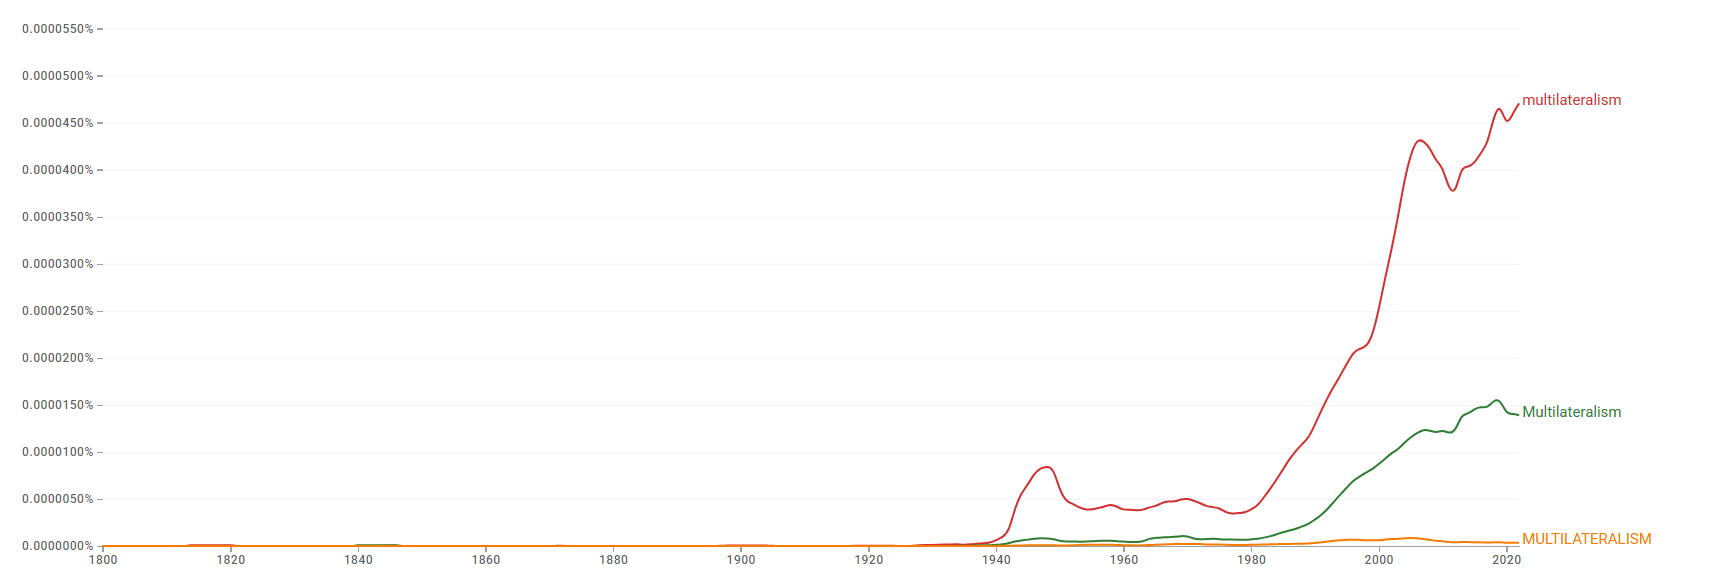
\includegraphics[width=0.75\textwidth]{img/googlengram_english.png}
\caption{Pourcentage d'occurrences de \textit{multilateralism} sur Google Ngram }
\end{figure}


\begin{figure}
\centering %
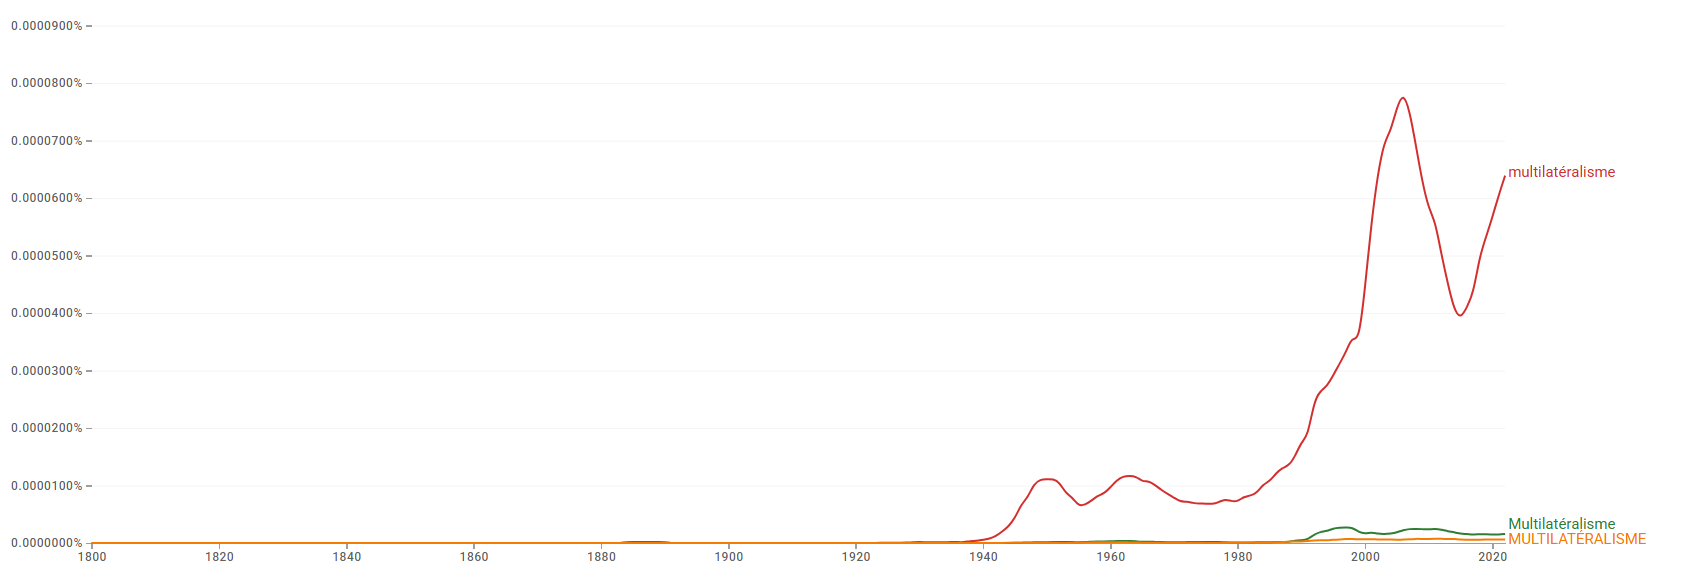
\includegraphics[width=0.75\textwidth]{img/googlengram_french.png}
\caption{Pourcentage d'occurrences de \textit{multilatéralisme} sur Google Ngram}
\end{figure}

Par ailleurs, des visions similaires aux principes représentatifs du multilatéralisme contemporain, telles que la concertation et la solidarité entre États, étaient déjà présentes dans certaines initiatives et événements politiques antérieurs, par exemple le mouvement Paneuropa proposé par Richard Coudenhove-Kalergi, la Société des Nations après la Première Guerre mondiale, voire l'Union télégraphique internationale encore plus tôt. La continuité et l'évoultion idéologiques entre ces actes politiques semblent toutes deux indiquer un fait : le multilatéralisme, en tant que concept et esprit, n'a pas été exclusivement défini à travers les normes établies après la Seconde Guerre mondiale ; au contraire, ses fondements et ses prémices étaient déjà profondément enracinés dans les interactions de la communauté internationale et même dans la conscience publique bien avant cette époque. Cela nous amène à poser une nouvelle question : avant sa définition formelle, peut-on considérer que le multilatéralisme substantiel existait déjà ? Et si oui, à quel moment précis est-il apparu ?

Pour répondre à cette question, il est nécessaire de déplacer la focale de l'examen des seuls faits historiques relatifs aux interactions interétatiques vers une analyse plus fine des processus décisionnels. La France constitue sans doute un excellent exemple. D'une part, elle a participé à presque tous les grands processus politiques internationaux du XIX\textsuperscript{e} siècle jusqu'à la Seconde Guerre mondiale. D'autre part, la France a longtemps été un pays dominé par son Parlement, où le système délibératif jouait un rôle majeur dans les décisions politiques, y compris en matière de politique étrangère, et où le Parlement faisait office de passerelle entre l'opinion publique et la décision politique. En d'autres termes, si des idées ou conceptions multilatéralistes existaient déjà, elles ont nécessairement laissé des traces dans les débats parlementaires. L'étude du contenu de ces débats peut donc nous aider à situer avec plus de précision la réponse à notre question.

Une difficulté subsiste toutefois : face à l'ampleur considérable des archives parlementaires, une lecture exclusivement humaine mobiliserait un temps et une énergie immenses. Comment alors extraire rapidement et efficacement les éléments pertinents depuis ces textes ? Heureusement, le développement rapide de l'intelligence artificielle et des modèles de langage a rendu possible une "lecture" automatisée. Parmi ces avancées, une technologie particulièrement représentative est celle de la génération augmentée par récupération. Son principe central est d'intégrer une base de données externe dans le processus de génération d'un grand modèle de langage, de sorte que l'utilisateur puisse demander à celui-ci de produire une réponse à partir du contenu de cette base. Cependant, l'application de cette technologie dans le domaine de la recherche historique reste encore largement à éprouver, tant sur le plan technique que théorique.

En basant sur tout ce que nous avons discuté précédemment, cette recherche vise à répondre à deux questions principales :
\begin{enumerate}
    \item Comment le multilatéralisme se manifeste-t-il au sein du Parlement français ? À défaut, comment celui-ci perçoit-il et traite-t-il les questions de politique internationale ?
    \item Comment les technologies de type génération augmentée par récupération peuvent-elles être appliquées à la recherche historique ?
\end{enumerate}

Notre recherche se concentre sur la période 1929-1939 en France, couvrant des événements majeurs allant du déclenchement de la Grande Dépression au début de la Seconde Guerre mondiale. Cette période occupe une place déterminante dans l'histoire diplomatique. Nous examinerons les archives des deux chambres du Parlement français, la Chambre des députés et le Sénat, à l'aide des technologies d'intelligence artificielle, notamment la génération augmentée par récupération, afin de tenter de répondre aux deux questions ci-dessus.  

La structure de cette recherche est la suivante : dans une première partie, nous nous concentrerons sur le Parlement et le multilatéralisme, en passant en revue, à partir des études existantes, certaines caractéristiques du Parlement à cette époque, puis en discutant de la Société des Nations et des activités diplomatiques à caractère multilatéral durant cette période. Dans une deuxième partie, nous aborderons davantage les aspects techniques : nous présenterons les méthodes d'intelligence artificielle et de traitement automatique du langage utilisées, ainsi que leur application dans des recherches antérieures, puis nous décrirons le corpus utilisé, les procédés de traitement des données et leurs limites. Dans la partie consacrée aux résultats, nous exposerons les éléments dégagés des données et nous les illustrerons au moyen de nombreuses figures et graphiques. Enfin, dans la conclusion, nous résumerons cette recherche, discuterons de ses limites et proposerons des perspectives pour des travaux futurs.


\chapter{Partie I}
\section{Le Parlement entre les deux guerres}
Lorsqu'on cherche à comprendre la manière dont les enjeux de politique internationale sont présentés et reçus au sein du Parlement, il est indispensable de prendre en compte les conditions "matérielles" qui les sous-tendent, à savoir le mode d'organisation institutionnelle du Parlement. Or, avec le temps, ce mode d'organisation connaît des évolutions diachroniques, dues à divers facteurs internes et externes, ce qui rend nécessaire une analyse dynamique de cette institution. Dans le contexte français, ce phénomène peut être appréhendé à travers trois axes d'analyse : l'évolution des rapports de force entre le gouvernement et le Parlement, les relations entre le Sénat et le Chambre des députés, ainsi que la coopération et les conflits entre partis appartenant à différents spectres politiques au sein du Parlement. Nous allons examiner chacun de ces aspects dans les sections qui suivent.

\subsection{L'évolution des relations entre le gouvernement et le Parlement}
Depuis la Révolution française, la relation entre le gouvernement et le parlement peut être considérée comme un baromètre des évolutions institutionnelles, marquée par une transition permanente.
Aux XVIII\textsuperscript{e} et XIX\textsuperscript{e} siècles, cette relation a connu des oscillations marquées. À l'origine de l'Assemblée nationale, le pouvoir législatif détenait une autorité suprême sur l'exécutif\footcite[p.37]{morel2024}. Cependant, avec la Restauration, les prérogatives parlementaires furent confinées à un suffrage restreint, n'étant plus qu'une garantie minimale et précaire\footcite[p.125]{morel2024}. La Deuxième République vit l'émergence d'un véritable régime parlementaire, posant les bases des institutions futures. Ce fut une période durant laquelle des droits tels que le droit d'enquête parlementaire, le droit d'interpellation ou encore la motion de censure furent effectivement exercés\footcite[p.154]{morel2024}, et où furent rétablies la présidence tournante de la Chambre ainsi que l'adoption de systèmes de vote plus stables au sein de la Constituante\footcite[p.157]{morel2024}.
Malgré une limitation initiale des pouvoirs parlementaires sous le Second Empire, une inflexion s'amorça dès 1857. À la fin de l'Empire et avec l'avènement de la Troisième République, notamment après la promulgation des lois constitutionnelles du 25 février 1875, le parlementarisme fut renforcé (nous y reviendrons dans les sections suivantes), consolidant la supériorité du législatif sur l'exécutif. En somme, avant la Première Guerre mondiale, à l'exception de certaines périodes de bouleversements politiques, le pouvoir législatif était généralement dominant, et, grâce à une consolidation institutionnelle progressive, la France s'imposa comme une véritable république parlementaire.

La Grande Guerre marqua toutefois, quoique brièvement, une inflexion dans ce rapport : le gouvernement vit son rôle renforcé par rapport au parlement. Ainsi, le droit exclusif de l'assemblée de débattre de son ordre du jour fut suspendu ; la Chambre devait statuer immédiatement sur les propositions du gouvernement\footcite[p.227]{morel2024}.

Dans l'immédiat après-guerre, on assista à un retour à une république parlementaire plus traditionnelle. La relation entre l'exécutif et le législatif fut alors caractérisée par une "distance constitutive"\footcite[p.341]{zotero-515}, obligeant le gouvernement à respecter les prérogatives parlementaires. Par exemple, Millerand dut s'engager à ne pas mener de diplomatie secrète pour obtenir la majorité parlementaire. Toutefois, ce soutien parlementaire restait fragile : il ne garantissait pas au gouvernement la continuité dans ses politiques et ses réformes internes\footcite[p.343]{zotero-515}. Cette instabilité s'explique avant tout par les traditions de vote parlementaire persistantes et par la structure organisationnelle des partis politiques. Un gouvernement privé de la confiance du parlement se retrouvait rapidement paralysé par le législatif.

La victoire du Cartel des gauches en 1924 marqua un retour aux traditions du parlementarisme triomphant, dans l'esprit de la "république radicale" des années 1900. La doctrine radicale plaçait le parlement au centre des institutions. Les autres composantes du Cartel considéraient la démocratie républicaine comme indissociable du parlement, rejetant tant le renforcement de l'exécutif que toute forme alternative d'expression démocratique\footcite[p.347]{zotero-515}. Durant cette période, le soutien parlementaire était jugé essentiel pour toute initiative gouvernementale. Les délégations parlementaires s'efforçaient de forger des majorités (en l'occurrence, celle de gauche), et le gouvernement s'abstenait de demander de longs débats sans leur accord\footcite[p.348]{zotero-515}.

Cependant, dès la fin des années 1920, cette relation se modifia de nouveau, notamment sous l'effet de la crise du franc. Celle-ci entraîna la fragmentation du Cartel : les radicaux privilégiaient la défense des intérêts bourgeois, tandis que les socialistes insistaient sur la discipline de parti. Cette crise budgétaire et financière n'affecta pas seulement l'économie, mais révéla également un dysfonctionnement du système parlementaire. La divergence idéologique entre les factions empêchait toute réponse concertée, ouvrant la voie à une polarisation accrue\footcite[p.349]{zotero-515}. L'arrivée de Poincaré visait à restaurer une certaine cohésion parlementaire. En réalité, la plupart des mesures de redressement furent définies par le gouvernement de Poincaré, le parlement se contentant de les entériner. Poincaré recourut à des moyens coercitifs pour forcer le parlement à accepter ses décisions, soulignant ainsi la faiblesse du parlement en temps de crise et annonçant une évolution future des rapports entre exécutif et législatif.

Dans les années 1930, plusieurs facteurs affectèrent cette dynamique. La Grande Dépression de 1930-31 frappa la France, mais les divergences entre parlementarisme traditionnel et modernisation des partis empêchèrent toute réponse unifiée\footcite[p.352]{zotero-515}. Les successeurs de Poincaré, tels Laval ou Tardieu, privés de son prestige, durent recourir aux décrets-lois pour préserver une cohésion fragile au sein du parlement. Puis survint la crise du 6 février 1934. Bien qu'empreinte d'une forte connotation droitière, cette crise fut avant tout l'expression du mécontentement populaire face au parlementarisme depuis la crise économique. Elle constitua un tournant, en marquant pour la première fois une opposition directe entre le parlement et le peuple\footcite[p.356]{zotero-515}. Désormais, tant la gauche que la droite cessèrent de considérer le parlement comme le principal vecteur de leur action politique, cherchant à le contourner par d'autres moyens.

Sous l'égide du gouvernement Doumergue, la République tenta diverses réformes institutionnelles, souvent fondées sur la création d'organismes alternatifs, afin de marginaliser le parlement. Bien que ces projets échouèrent en raison des divisions internes, ils révélèrent la précarité du parlement. Contrairement à son rôle central antérieur, le parlement des années 1930 sombra dans l'impuissance. Le fonctionnement de la République dépendait alors largement des décrets-lois\footcite[p.365]{zotero-515}, et le parlement délégua son rôle traditionnel à l'exécutif.

En conclusion, le parlementarisme, florissant depuis le XIX\textsuperscript{e} siècle, vit son influence décliner significativement à la fin des années 1920 et dans les années 1930. Le gouvernement s'affirma progressivement, phénomène attribuable à une conjonction de facteurs : crises économiques, polarisation idéologique des factions parlementaires, et modernisation du système partisan. Cette évolution ne manqua pas d'avoir un impact profond sur la manière dont les questions internationales furent débattues et résolues au sein du parlement.


\subsection{L'évolution des relations entre le Sénat et la Chambre des députés}
Comprendre l'évolution des relations entre le Sénat et la Chambre des députés est une étape cruciale pour saisir la transformation du rôle du Parlement lui-même. Contrairement au régime précédent, qui reposait sur un système polycaméral à trois assemblées\footcite[p.167]{morel2024}, la Troisième République établit un bicamérisme par la loi du 25 février 1875. Celui-ci se composait d'une Chambre des députés, dont les membres étaient élus au suffrage universel, et d'un Sénat, issu d'un suffrage plus restreint. La loi du lendemain vint préciser les compétences respectives des deux chambres, confiant par exemple à la Chambre des députés l'examen des lois financières, tandis que le Sénat se voyait par exemple attribuer la compétence sur les crimes contre la sûreté de l'État et les actes de haute trahison.

Durant la période précédant la Première Guerre mondiale, l'histoire parlementaire fut marquée par une collaboration généralement harmonieuse entre les deux chambres, bien que ponctuée de tensions occasionnelles. En règle générale, la coopération entre les chambres reposait sur le respect de certaines conventions assurant le bon fonctionnement du régime. En cas de désaccord, le Sénat finissait le plus souvent par céder, sauf lorsqu'il s'agissait de questions fondamentales touchant aux institutions ou aux idéologies\footcite[p.196]{morel2024}. À cet égard, la Chambre des députés jouissait d'un poids politique supérieur à celui du Sénat. En ce qui concerne les rapports entre le gouvernement et le Parlement, le gouvernement devait bénéficier de l'aval d'au moins l'une des deux chambres pour exercer le pouvoir, et demeurait responsable devant le Sénat\footcite[p.197]{morel2024}.

Si l'on se tourne vers la période entre les deux guerres mondiales, on constate qu'après la guerre, toutes les assemblées républicaines furent renouvelées par des élections. Le Sénat conserva une certaine continuité, les radicaux-socialistes et les républicains de gauche, forces dominantes avant-guerre, y conservèrent leurs sièges\footcite[p.337]{zotero-515}. En revanche, la Chambre des députés connut une transformation plus profonde de sa composition : les partis de gauche et le parti radical-socialiste furent les grands perdants de cette élection, la gauche échouant pour la première fois à remporter une majorité\footcite[p.338]{zotero-515}. Une part importante des nouveaux députés étaient d'anciens combattants, souvent engagés politiquement à l'échelle locale avant leur mobilisation. Ces hommes apportèrent un style nouveau à la Chambre : ils cherchèrent à y maintenir l'esprit d'Union sacrée, optant pour des interventions brèves et concises, tandis que ceux qui continuaient à pratiquer de longs discours dans le style d'avant-guerre suscitaient la méfiance\footcite[p.339]{zotero-515}. Cette dynamique contrastait avec celle des divers groupes constituant le Bloc national, contribuant à une complexité politique interne à la Chambre.

Dans les années 1920, l'équilibre entre les deux chambres se reflétait clairement dans le processus législatif. L'initiative législative appartenait au gouvernement, qui préparait les premières études des projets de loi et orientait les débats parlementaires. Le rôle du Parlement consistait alors à débattre et à amender ces textes. À ce stade, la coopération entre la Chambre et le Sénat était manifeste : les amendements proposés par l'une étaient généralement acceptés par l'autre. Un certain "non-dit" institutionnel facilitait ces échanges : la Chambre approuvait la majorité des modifications apportées par le Sénat, et en cas de désaccord, ce dernier choisissait souvent de se retirer afin d'éviter de bloquer l'avancée législative\footcite[p.345]{zotero-515}.

Cependant, cette dynamique ne dura pas. À partir du milieu des années 1920, les crises du franc et du budget affectèrent profondément les équilibres politiques. Le Cartel des gauches, alors dominant, se fractura en raison de désaccords internes. Cette désunion se manifesta également dans les relations entre les deux chambres : chacune rejeta ou modifia systématiquement les propositions de l'autre\footcite[p.349]{zotero-515}, rompant ainsi avec la politesse institutionnelle habituelle. Les mesures économiques proposées par la Chambre étaient jugées trop ambitieuses par le Sénat et donc rejetées. De plus, les divergences s'accentuèrent sur les questions de politique étrangère et du traité de Versailles\footcite[p.235]{morel2024}, et il fallut attendre l'arrivée de Poincaré au pouvoir pour voir s'amorcer une stabilisation.

Dans les années 1930, la polarisation idéologique contribua à accentuer la fragmentation interne du Parlement : au Luxembourg, l'univers du radicalisme et du parlementarisme délibératif ; au Palais-Bourbon, celui, en pleine accélération, des grands partis de masse et des idéologies\footcite[p.237]{morel2024}. Après la formation du gouvernement Blum, celui-ci parvint dans un premier temps à obtenir une majorité au sein de la Chambre et à instaurer un consensus entre la Chambre et le Sénat, permettant le passage rapide de plusieurs réformes sociales et économiques. Mais après quelques mois, cette dynamique se heurta au Sénat, qui réclama un retour à une méthode plus délibérative, fondée sur la prudence et le respect du débat parlementaire\footcite[p.364]{zotero-515}.

En somme, les relations entre les deux chambres du Parlement français peuvent être vues comme le reflet d'un réseau complexe de rapports de pouvoir. Elles influencent et sont influencées par les dynamiques entre pouvoir exécutif et législatif, ainsi que par les relations internes la Chambre et le Sénat, qu'il s'agisse de celles entre partis, factions ou même individus. Comme nous l'avons vu, le passage d'un fonctionnement basé sur la convention et l'harmonie vers une ère de conflits et d'oppositions reflète également une transformation des relations entre le gouvernement et le Parlement. Pour comprendre pleinement cette évolution, il convient d'examiner plus en détail les transformations dans l'équilibre des forces idéologiques et partisanes au sein même du Parlement, un sujet que nous aborderons dans la section suivante.

\subsection{L'évolution des rapports de force entre les partis politiques au sein du Parlement}
Comparés aux divers facteurs évoqués dans les deux premières sections, les évolutions idéologiques et les changements institutionnels survenus au sein du Parlement durant la Troisième République et après la Première Guerre mondiale ont exercé une influence plus fondamentale sur la manière dont le Parlement, en tant qu'ensemble, aborde les questions concrètes.

L'émergence de groupes politiques, voire de partis, est une caractéristique majeure du Parlement français au XX\textsuperscript{e} siècle. Contrairement aux factions traditionnelles telles que les royalistes ou les républicains, ces nouveaux groupements politiques se sont inscrits pour la première fois dans une reconnaissance formelle. En 1910, il fut ainsi décidé que chaque groupe remettrait, en début de session, une liste de ses membres au président de la Chambre, liste qui devait ensuite être publiée dans le Journal officiel. Ce fut effectivement le cas le 6 juillet 1910. En 1915, les sièges des députés furent attribués par groupe, alors qu'auparavant ils étaient répartis au fur et à mesure de leur libération, selon l'ancienneté des parlementaires\footcite[p.218]{morel2024}. Avant 1910, les députés agissaient presque exclusivement en fonction de leur volonté individuelle, mais à partir de ce moment-là, le groupe devient un intermédiaire essentiel entre les parlementaires et les institutions. La création en 1911 de la Conférence des présidents en est une autre illustration : cette instance réunit les présidents des groupes, les présidents de commissions et les membres du gouvernement pour fixer l'ordre du jour. Par ailleurs, la reconnaissance des groupes a également transformé le mécanisme du vote, certains membres pouvant voter au nom de leur groupe\footcite[p.219]{morel2024}, ce qui constitue une rupture nette avec les pratiques du parlementarisme délibératif et libéral d'avant.

Dès l'avant-guerre, on pouvait observer certaines ruptures internes au Parlement dues à l'existence de ces groupes. Outre les désaccords généraux entre partis, la prolifération des groupes politiques rendait les lignes idéologiques internes à un même parti beaucoup plus anfractueuses, rendant difficile l'adoption d'une position commune. Par ailleurs, la présence de groupes d'intérêt compliquait davantage l'unité parlementaire\footcite[p.220]{morel2024}. Pendant la Première Guerre mondiale, les forces politiques au sein du Parlement se réconcilièrent sous le mot d'ordre de l'Union sacrée, un climat qui se prolongea après la guerre : comme mentionné précédemment, une part importante des parlementaires élus avaient servi dans l'armée pendant le conflit, et beaucoup espéraient poursuivre la tradition d'unité nationale. Cependant, cette aspiration ne fut pas toujours effective, et les groupes politiques restaient des structures puissantes.

Sous le gouvernement Millerand, la séparation entre le pouvoir exécutif et le pouvoir législatif fut maintenue, notamment parce que la majorité des députés tenaient à préserver leur liberté de vote. Le Parlement français ne vit donc pas l'émergence généralisée de partis véritablement modernes, capables d'imposer leur discipline de vote à leurs membres\footcite[p.342]{zotero-515}. Une exception notable fut la Section française de l'Internationale ouvrière (SFIO), qui, après le congrès de Tours, introduisit une nouvelle conception de la représentation : le député communiste devait avant tout être le représentant du parti, et son vote devait être guidé par un sentiment d'appartenance fondé sur la conscience de classe\footcite[p.238]{morel2024}.

L'absence généralisée de partis puissants signifiait aussi que la représentation nationale était encore assimilée à la "nation assemblée", concept fondé à la fois sur la conscience individuelle des sénateurs et députés, et sur la conscience collective de la Chambre et du Sénat\footcite[p.344]{zotero-515}.

La victoire du Cartel des gauches en 1924 permit une certaine unité au sein du Parlement, mais cette unité fut rapidement brisée par les crises budgétaires et la chute du franc. Le Cartel fut divisé entre les radicaux, qui voulaient défendre les intérêts de la classe moyenne, et les socialistes, soucieux de préserver leur orthodoxie idéologique\footcite[p.349]{zotero-515}. Lors des débats sur les projets de réforme, des divergences idéologiques apparurent : les radicaux voulaient maintenir les principes du libéralisme économique, tandis que les socialistes proposaient des solutions d'inspiration marxiste. Le recours à la discipline de vote des partis pour obtenir la majorité suscita également le mécontentement de plusieurs députés. Par conséquent, les propositions fiscales et budgétaires teintées de socialisme rencontrèrent de fortes oppositions au sein du Parlement\footcite[p.350]{zotero-515}. Ce scénario se répéta dans la coalition radicaux-socialistes en 1932. Globalement, les tensions parlementaires de cette époque révèlent une opposition structurelle entre les formes d'organisation des partis modernes et celles des partis de type pré-moderne.

À partir de 1924, le Parlement oscille entre les anciennes traditions parlementaires et la logique des partis modernes. Pour ceux du centre droit attachés au parlementarisme traditionnel, les radicaux portaient atteinte au Parlement, puisque le maintien ou le retrait des ministres dépendait désormais des congrès de parti et non de la décision de parlementaire, conférant à la souveraineté du parti une supériorité sur la souveraineté parlementaire. Pour les partisans de la modernisation parlementaire, la montée en puissance des partis était une bonne chose, car ils voyaient l'instabilité des majorités comme la cause de l'instabilité gouvernementale. À gauche, on estimait que les partis devaient donner aux électeurs l'image d'une alliance stable tout au long de la législature, afin d'exprimer la volonté populaire. Mais cette tension entre instabilité parlementaire et nécessité d'un gouvernement fort resta non résolue, surtout après l'arrivée de la Grande Dépression.

Dès le milieu des années 1920, on constate au sein du Parlement des désaccords sur de nombreuses réformes. Par exemple, la réforme Joseph-Barthélemy de 1926 visait à encadrer le temps de parole et les conditions d'intervention à la tribune, réservant ce droit à ceux reconnus par leur groupe. Mais cette réforme échoua à cause d'une méfiance persistante entre groupes : la gauche craignait un gouvernement autoritaire maîtrisant les débats parlementaires, tandis que les centristes refusaient qu'un seul parti puisse manipuler le Parlement\footcite[p.355]{zotero-515}.

La crise du 6 février 1934 accentua les divergences entre gauche et droite. Doumergue, appelé à la tête du gouvernement, fit de la réforme de l'État une priorité. Sous ce terme se cachaient plusieurs mesures visant à réduire le rôle du Parlement au profit de l'exécutif\footcite[p.357]{zotero-515}, des mesures marquées idéologiquement à droite. Pour la droite, un État fort ne peut coexister avec une République parlementaire. Cette volonté provoqua une réaction immédiate de la gauche, qui refusa toute réforme de l'État et chercha à défendre les institutions républicaines. Ce clivage idéologique paralysa le Parlement, rendant impossible la réforme constitutionnelle souhaitée par Doumergue.

Ce blocage entraîna un autre problème : l'extrême polarisation du Parlement l'empêchait de répondre efficacement à la crise économique. Gauche et droite s'opposaient sur la nécessité d'utiliser des outils administratifs puissants pour gérer la crise. La gauche craignait une dérive autoritaire. Même après l'arrivée au pouvoir du Front populaire et les réformes rapides menées par Blum, le ralentissement des débats incita la gauche à réclamer des pleins pouvoirs financiers et économiques\footcite[p.364]{zotero-515}.

À la fin des années 1930, le Parlement s'était pratiquement figé. Son rôle fut remplacé par celui d'un gouvernement fort. Sur les questions de politique étrangère, il n'opposa plus de résistance. Cette évolution fut le fruit d'un long processus : montée en puissance des partis, polarisation idéologique, divisions internes à chaque camp, et affirmation progressive d'un exécutif renforcé. Sur cette base, on peut anticiper une transformation profonde dans la manière dont les opinions individuelles et collectives sont reçues et exprimées au sein du Parlement.


\section{L'histoire du multilatéralisme}
\subsection{La définition et évolution du concept de multilatéralisme}
Ce qui nous intéresse tout d'abord, c'est le multilatéralisme et l'évolution historique de ses concepts connexes.
Bien que le terme "multilatéralisme" lui-même n'ait émergé qu'après la Seconde Guerre mondiale, ses pratiques et principes fondamentaux, ainsi qu'un concept qui lui est étroitement lié, la diplomatie multilatérale, possèdent une histoire bien plus ancienne\footcite{library}. Par définition, la diplomatie multilatérale implique des relations entre au moins trois États. Mais dans la pratique, elle rassemble souvent des dizaines de pays ainsi que, potentiellement, des acteurs non étatiques, pour traiter une grande variété de sujets : guerre et paix, droits de l'homme, commerce, environnement, etc. \footcite[p.35]{petiteville2020}.

La diplomatie multilatérale a une longue histoire, et l'on considère généralement que le traité de Westphalie en constitue le prototype moderne \footcite{chikvaidze2020}. Plus de cent représentants des puissances belligérantes y participèrent, donnant lieu à une des premières formes de conférence diplomatique axée sur la paix.

Le Congrès de Vienne de 1815 et le système dit du "Concert européen" marquèrent une étape importante dans le développement de la diplomatie multilatérale. Après les guerres napoléoniennes, les principales puissances européennes mirent en place un mécanisme informel de concertation pour maintenir l'ordre. Bien que de portée limitée et non institutionnalisé, ce mécanisme habitua les grandes puissances à se rencontrer avant que les conflits n'éclatent, ouvrant ainsi la voie aux futures conférences internationales \footcite{library}. Ce système, bien que dominé par les grandes puissances et peu formel, incarnait déjà certains éléments multilatéraux, tels que l'indivisibilité de la paix entre ses membres et l'obligation non discrétionnaire de réagir face à des actes d'agression. Il permit aux cinq grandes puissances (Autriche, Royaume-Uni, Prusse, Russie et France) d'éviter une logique de maximisation de puissance relative, établissant ainsi une norme de stabilité systémique\footcite[p.578-579]{ruggie1992}.

Par la suite, les conférences de la paix de La Haye, en 1899 et 1907, marquèrent un nouveau jalon de la diplomatie multilatérale. D'un côté, elles réunirent la majorité des pays du monde ; de l'autre, elles furent les premières tentatives internationales pour établir des mécanismes destinés à prévenir la guerre\footcite{library}.

La création de la Société des Nations après la Première Guerre mondiale représente un tournant majeur dans l'évolution de la diplomatie multilatérale. Il s'agissait de la première organisation internationale visant à préserver la paix et à promouvoir la coopération entre les nations\footcite{library}. Le Pacte de la Société des Nations établissait des principes tels que la solidarité, le respect de la souveraineté, l'égalité des droits, la consultation collective, la transparence, le règlement pacifique des différends et la primauté du droit international. Plus encore, il offrait un cadre multilatéral permanent permettant aux États membres de se réunir régulièrement sur un pied d'égalité\footcite{library}. Ce cadre couvrait un large éventail de questions politiques et techniques, et les acteurs non étatiques, comme les associations privées, y jouaient également un rôle actif.

La définition du multilatéralisme reste en continuité avec celle de la diplomatie multilatérale. Au-delà du simple critère numérique, le multilatéralisme met l'accent sur l'adhésion à un projet politique commun fondé sur le respect d'un système partagé de normes et de valeurs\footcite{library}. J. G. Ruggie\footcite[p.571]{ruggie1992} va plus loin en définissant le multilatéralisme comme une forme institutionnelle générique dans les relations internationales, une forme basée sur des principes de comportement "universels" régissant les actions des États, indépendamment de leurs intérêts spécifiques ou de l'urgence stratégique d'un contexte particulier. Dans ce cadre, les actions des États sont marquées par l'indivisibilité et génèrent des attentes de réciprocité diffuse, c'est-à-dire une anticipation de bénéfices mutuels équitables à long terme.

Ainsi, la distinction essentielle entre le multilatéralisme, la diplomatie multilatérale et la coopération multilatérale réside dans le degré d'institutionnalisation. À ce titre, la Société des Nations peut être considérée comme la première manifestation substantielle du multilatéralisme. Bien qu'elle n'ait pas réussi à empêcher la Seconde Guerre mondiale, elle a laissé un héritage structurel important pour le système international et jeté les bases d'un multilatéralisme plus institutionnalisé et mature. En 1945, avec la création de l'Organisation des Nations Unies (ONU), le multilatéralisme est entré dans une nouvelle phase de développement, marquée par une institutionnalisation plus poussée. L'ONU a non seulement établi un ensemble de mécanismes formels de coopération internationale, mais elle a également instauré un système normatif universel fondé sur l'égalité souveraine, le règlement pacifique des différends et la sécurité collective\footcite{nationsa}. Ainsi, le multilatéralisme a été élevé du statut d'idée ou de tentative diplomatique à celui d'une pratique institutionnalisée au cœur des relations internationales. On peut affirmer que la fondation de l'ONU marque la transformation du multilatéralisme en une structure durable et systémique, faisant de cette organisation non seulement un produit de l'ordre international d'après-guerre, mais aussi une étape clé dans le processus d'institutionnalisation du multilatéralisme.

De manière générale, l'évolution et la mise en œuvre du concept de multilatéralisme reflètent la tendance progressive des relations internationales et de la diplomatie à se moderniser, à se structurer et à se normaliser. Par conséquent, le multilatéralisme n'est pas seulement une modalité d'action diplomatique, mais constitue également une pierre angulaire incontournable dans l'évolution du système international contemporain.

\subsection{Les pratiques multilatérales dans le cadre de la Société des Nations}

Comme mentionné précédemment, la Société des Nations (SDN) représente un tournant institutionnel dans le passage de la diplomatie multilatérale à un véritable multilatéralisme. De nombreuses pratiques diplomatiques entre les deux guerres mondiales se sont déroulées dans le cadre de la SDN.

Le système de la SDN reposait sur trois institutions principales : tout d'abord, l'Assemblée, qui se réunissait chaque année à Genève. Chaque État membre y disposait d'un maximum de trois délégués mais d'une seule voix. L'Assemblée établissait des commissions permanentes, élisait les membres non permanents du Conseil et les juges de la Cour permanente de justice internationale, et adoptait des résolutions ou émettait des recommandations. Ensuite, le Conseil, composé initialement de cinq membres permanents (France, Royaume-Uni, Italie, Japon — les États-Unis, bien que mentionnés, n'ont jamais adhéré) et de quatre membres non permanents (porté à six en 1922, puis à neuf en 1926). Le Conseil était chargé du maintien de la paix, de l'élaboration de plans de désarmement, de la médiation en cas de menace de conflit, et pouvait recommander des mesures militaires contre un agresseur. Les quatre membres permanents y exerçaient une influence dominante. Enfin, le Secrétariat préparait les documents et rapports pour l'Assemblée et le Conseil\footcite[p.37-38]{milza2019}. Outre ces institutions centrales, la SDN comptait de nombreux organes annexes, spécialisés dans des affaires politiques (tels que la Commission permanente des mandats, les Comités militaires et navals, le Haut-Commissariat pour les réfugiés) ou des questions techniques (tels que communications, coopération intellectuelle, questions sociales, esclavage, contrôle de l'opium)\footcite[p.39]{milza2019}.

En ce qui concerne les membres, la SDN fut initialement composée des puissances alliées signataires du traité de Versailles et de treize États neutres. Les puissances vaincues, notamment l'Allemagne, furent d'abord exclues. Tout État souverain acceptant les obligations de la SDN pouvait devenir membre, par un vote des deux tiers de l'Assemblée. Les États pouvaient se retirer en prévenant deux ans à l'avance, ou être exclus par un vote unanime du Conseil et de l'Assemblée. Les États-Unis ne rejoignirent jamais la SDN, leur Sénat refusant de ratifier le traité de Versailles incluant le Pacte de la Société. L'Allemagne, l'URSS, ainsi que plusieurs pays d'Amérique latine, quittèrent ou cessèrent ultérieurement de participer activement à la SDN\footcite[p.36-37]{milza2019}.

Pendant une certaine période après la guerre, la France fut un fervent promoteur de la diplomatie multilatérale dans le cadre de la SDN. Après 1924, sous la direction d'Édouard Herriot, la politique étrangère française évolua d'une logique de sécurité unilatérale vers une approche de sécurité collective, visant à établir des relations de sécurité avec des adversaires potentiels par des accords multilatéraux, plutôt que par des alliances traditionnelles. En septembre 1924, lors d'une session de la SDN, Herriot lança le triptyque "arbitrage, sécurité, désarmement", et fut à l'origine du Protocole pour le règlement pacifique des différends internationaux, qui prévoyait un arbitrage obligatoire et des sanctions militaires contre les agresseurs. Cependant, le refus britannique entraîna l'échec du protocole\footcite[p.455]{guieu2016}.

En février 1932, la Conférence du désarmement s'ouvrit à Genève sous l'égide de la SDN, avec la participation de 62 États, y compris les États-Unis et l'URSS. Plusieurs plans furent proposés : le plan Tardieu de la France (force internationale, arbitrage obligatoire), le plan Hoover des États-Unis (suppression des armes offensives, réduction d'un tiers des armements). Mais les priorités nationales prévalurent : l'Allemagne réclamait l'égalité des droits, tandis que la France et le Royaume-Uni cherchaient à préserver leur supériorité militaire\footcite[p.142]{milza2019}. En décembre 1932, la France accepta le principe d'égalité de traitement pour l'Allemagne. Pourtant, en octobre 1933, Hitler fit quitter à l'Allemagne la conférence et la SDN, afin de pouvoir réarmer librement\footcite[p.146-147]{milza2019}.

La France utilisa aussi les mécanismes de coopération multilatérale de la SDN pour promouvoir sa culture, notamment par le Comité international de coopération intellectuelle et l'Institut international de coopération intellectuelle à Paris. Cette initiative visait à améliorer l'image de la France et de sa culture, bien que certains pays, comme le Royaume-Uni, l'aient perçue comme un outil d'impérialisme culturel français\footcite[p.411]{guieu2016}.

Par ailleurs, la SDN supervisait les anciens territoires coloniaux, notamment ceux de l'Empire ottoman et de l'Empire allemand, dans le cadre du système des mandats. Ces territoires furent classés en mandats de type A (comme la Syrie et le Liban, supposés rapidement indépendants) et mandats de type B (ex-colonies allemandes en Afrique, jugées moins développées)\footcite[p.80]{montero2001}\footcite[p.286-287]{guieu2016}. Sur le plan économique, la SDN joua un rôle d'assistance : en 1922, elle aida l'Autriche en difficulté, et son Organisation économique et financière contribua à stabiliser la monnaie des jeunes États européens\footcite[p.43]{milza2019}. 

Cependant, la SDN fut confrontée à de nombreux défis. L'agression japonaise en Mandchourie en est un exemple marquant. Sous la présidence de Briand, la SDN reconnut d'abord les "mesures de sécurité" invoquées par le Japon, puis envoya la Commission Lytton, dont le rapport dénonça la création de l'État du Mandchoukouo, tout en suggérant une autonomie interne au sein de la Chine. L'Assemblée adopta ce rapport, mais le Japon refusa de s'y conformer et quitta la SDN en mars 1933\footcite[p.138-139]{milza2019}. Les grandes puissances, dont la France et les États-Unis, refusèrent toute action ferme, préférant défendre leurs intérêts propres à la logique de sécurité collective\footcite[p.140-141]{milza2019}.

Ensuite, l'agression italienne contre l'Éthiopie, membre de la SDN, révéla encore davantage la faiblesse de l'organisation. Bien que l'Italie fut reconnue comme agresseur et que des sanctions économiques soient votées, leur application fut limitée par le manque de volonté française, la peur britannique d'un conflit, et le non-respect des sanctions par d'autres puissances comme l'Allemagne et les États-Unis\footcite[p.181]{milza2019}.

Lorsque Hitler remilitarisa la Rhénanie en violation du traité de Versailles, les démocraties européennes réagirent timidement. La France porta l'affaire devant la SDN, mais le Royaume-Uni refusa tout soutien militaire, affirmant qu' "il n'y avait heureusement aucune raison de supposer que la présente action de l'Allemagne comporte une menace d'hostilités"\footcite[p.186]{milza2019}. Cela mit en lumière l'impuissance de la SDN et la faiblesse des démocraties face à l'agression.

Si le cadre de la SDN incarnait de nobles idéaux de paix et de coopération, il fut fondamentalement limité par les intérêts nationaux et le réalisme des grandes puissances. Celles-ci plaçaient souvent leur sécurité et leurs intérêts économiques au-dessus des principes de sécurité collective. Par exemple, les États-Unis privilégiaient la reconstruction économique de l'Europe et leurs intérêts financiers ; le Royaume-Uni visait à maintenir un équilibre, en évitant une hégémonie française\footcite[p.51-52]{milza2019}\footcite[p.81]{montero2001}. La France elle-même oscillait entre fermeté et compromis, tiraillée entre préoccupations sécuritaires et divisions internes\footcite[p.81]{montero2001}. L'essor de régimes autoritaires agressifs en Allemagne, en Italie et au Japon, qui rejetaient les traités et poursuivaient le réarmement et l'expansion territoriale, porta un coup fatal au système de la SDN. Le refus des démocraties de réagir avec fermeté, combiné à leurs divisions et au pacifisme ambiant, donna naissance à la politique d'apaisement, qui affaiblit encore davantage le système de sécurité collective. La Grande Dépression nuisit gravement à la coopération internationale, alimentant le nationalisme économique (protectionnisme, autarcie des régimes totalitaires) et le chacun-pour-soi. Un tel contexte entravait les efforts de solutions communes ou de désarmement.

Malgré l'esprit de Genève et l'adhésion populaire et politique à l'idée de paix par le droit\footcite[p.273]{guieu2016}, notamment en France, ces aspirations se heurtaient souvent aux exigences de la Realpolitik. La SDN, bien que dotée d'une structure innovante et d'un certain rôle, ne fut qu'un forum de coopération limitée, souvent instrumentalisée par les vainqueurs, et se révéla incapable face aux agressions des puissances révisionnistes.

\subsection{Les initiatives multilatérales en dehors de la Société des Nations}

Cette période a également vu l'émergence d'une série de pratiques diplomatiques multilatérales qui ont dépassé le cadre de la SDN. Fonctionnant parallèlement à la SDN, ces initiatives ont couvert de nombreux domaines et ont eu un impact profond sur les affaires internationales.

Sur le plan économique, plusieurs actions multilatérales fondées sur le système de Versailles ont été entreprises pour discuter et résoudre les problèmes liés aux réparations allemandes et à la crise économique. Il y eut d'abord la conférence de Londres sur le Plan Dawes, réunissant les Alliés (France, Royaume-Uni, États-Unis) et l'Allemagne, afin de réorganiser les paiements allemands. Cette conférence permit l'adoption du Plan Dawes, qui entraîna l'octroi de prêts internationaux à l'Allemagne, impliquant une forte influence financière anglo-américaine en Europe. Bien que fonctionnant en dehors du cadre formel de la SDN, cette initiative fut essentielle pour la stabilité économique européenne et posa les bases de l'adhésion ultérieure de l'Allemagne à la SDN\footcite[p.444-445]{guieu2016}. La conférence de La Haye en 1929 visait à finaliser le Plan Young, qui réduisit davantage les réparations allemandes et prévoyait le retrait anticipé des troupes alliées de la Rhénanie au 30 juin 1930\footcite[p.454]{guieu2016}.

Peu après, face à la Grande Dépression, le président américain Hoover proposa en 1931 un moratoire sur les dettes interétatiques, y compris les réparations allemandes, pour une durée d'un an\footcite[p.87]{montero2001}. Cette intervention financière multilatérale allait au-delà des attributions économiques habituelles de la SDN. À la suite de ce moratoire, la conférence de Lausanne de 1932 aboutit à l'abandon quasi total des réparations allemandes\footcite[p.87]{montero2001}. Ce fut une révision financière multilatérale majeure entre les grandes puissances. En 1933, la conférence économique de Londres tenta de trouver une réponse internationale à la crise économique mondiale, mais échoua largement à cause de profondes divergences entre les 66 pays participants, notamment le refus des États-Unis de stabiliser les taux de change\footcite[p.135]{milza2019}.

En parallèle, des conférences économiques régionales virent également le jour, comme celle d'Ottawa en 1932. Elle aboutit à une série d'accords commerciaux bilatéraux instaurant un système de préférence impériale au sein du Commonwealth, permettant la libre entrée ou des droits de douane réduits pour les marchandises échangées entre le Royaume-Uni et ses dominions\footcite[p.126-27]{milza2019}. Cela démontre en partie la préférence britannique pour le protectionnisme et le régionalisme économique plutôt que pour une coopération mondiale via la SDN.

En matière de sécurité et d'alliances militaires, les pratiques multilatérales furent encore plus diversifiées. La conférence navale de Washington (1921-1922), initiée par les États-Unis et réunissant les grandes puissances maritimes (États-Unis, Royaume-Uni, Japon, France, Italie), donna naissance au traité des Cinq Puissances limitant les armements navals\footcite[p.229-230]{guieu2016}. Cet effort important de désarmement multilatéral fonctionnait totalement en dehors de la SDN. La conférence navale de Londres de 1930 poursuivit cette logique.

Le Pacte de Locarno de 1925 réunissait l'Allemagne, la France, la Belgique, le Royaume-Uni et l'Italie. La France conclut également des traités de garantie avec la Pologne et la Tchécoslovaquie. Ces accords garantissaient l'inviolabilité des frontières entre la France, la Belgique et l'Allemagne, ainsi que la démilitarisation de la Rhénanie. Bien que Briand ait présenté ces traités comme un embryon constitutionnel d'une "famille européenne", ils créèrent en réalité une "sécurité différenciée" favorable à l'Ouest européen et établirent une "nouvelle coordination européenne" sous gestion des grandes puissances\footcite[p.447-448]{guieu2016}.

Le Pacte Briand-Kellogg de 1928, signé à Paris par 15 pays (puis par 63), visait à "mettre la guerre hors la loi" comme instrument de politique nationale. Bien qu'il ait reçu un accueil enthousiaste, il demeura principalement une déclaration morale, "sans sanctions prévues"\footcite[p.457-458]{guieu2016}, et manquait de mécanisme d'exécution par rapport aux clauses de sécurité collective de la SDN. Il s'agissait donc d'un engagement moral multilatéral hors du cadre opérationnel de la SDN.

Outre ces grands accords de sécurité, il existait aussi des pratiques diplomatiques multilatérales plus régionales et restreintes. Par exemple, la Petite Entente regroupait la Tchécoslovaquie, la Roumanie et la Yougoslavie, visant à empêcher le révisionnisme hongrois et un éventuel retour des Habsbourg\footcite[p.43]{milza2019}. Soutenue par la France, elle représentait un groupe d'alliés en Europe de l'Est indépendant de la SDN. En 1935, le Front de Stresa, une alliance diplomatique entre le Royaume-Uni, la France et l'Italie, visait à contrer l'agression hitlérienne, notamment en Autriche\footcite{mougel2018}. Il s'agissait d'un front de grandes puissances en dehors du cadre collectif universel de la SDN.

À la fin des années 1930, malgré la montée des tensions en Europe, on observe encore de nombreuses tentatives de diplomatie multilatérale et de sécurité collective : le pacte de non-intervention pendant la guerre civile espagnole (1936), les accords de Munich (1938), les garanties anglo-françaises envers les pays d'Europe de l'Est et les discussions militaires entre la France, le Royaume-Uni et l'URSS en 1939. Ces efforts, bien qu'intensifs, furent globalement voués à l'échec.

Étant donné que les États-Unis n'avaient jamais rejoint la SDN, les conférences panaméricaines initiées à partir de 1933 et la politique de bon voisinage de Washington représentaient un système multilatéral régional indépendant. Lors des conférences de Montevideo (1933), Buenos Aires (1936) et Lima (1938), les pays des Amériques réaffirmèrent leur solidarité et leur engagement pour la résolution pacifique des différends\footcite[p.220-221]{milza2019}.

Il existait aussi d'autres formes de coopération internationale. Le projet d'Union européenne proposé par Briand en 1929, bien que présenté devant l'Assemblée de la SDN, visait à créer un "lien fédéral" entre les peuples européens\footcite[p.465-466]{guieu2016}, avec des institutions européennes distinctes de la SDN. Cette initiative ambitieuse échoua en raison de la crise économique et du rejet par les États de toute forme de supranationalité\footcite[p.131]{milza2019}. Il y eut également les Congrès panafricains. Le premier, en 1919 à Paris, rassembla des représentants de communautés africaines et de la diaspora pour discuter d'autodétermination et d'égalité, plaidant pour un changement au sein du cadre colonial plutôt que contre celui-ci\footcite[p.303-304]{guieu2016}. Bien que moins formalisées que les accords de sécurité, ces initiatives représentent des formes significatives d'interaction internationale.

Ces initiatives variées soulignent la coexistence, et souvent la mise en concurrence, entre la diplomatie bilatérale traditionnelle, les groupes régionaux émergents et l'universalisme prôné par la SDN. Elles illustrent la complexité et la fragmentation des relations internationales durant l'entre-deux-guerres, les États cherchant fréquemment à résoudre les problèmes en dehors ou à la marge du système de la SDN.

\chapter{Partie II}

Dans cette partie, nous exposons les aspects techniques liés à cette recherche. Tout d'abord, nous présenterons les technologies mobilisées dans le cadre de cette étude et montrerons, à travers des exemples, comment elles peuvent être appliquées aux recherches en sciences humaines et sociales. Ensuite, nous détaillerons le pipeline de traitement des données utilisé dans cette recherche, en présentant les résultats obtenus pour évaluer sa performance, ainsi qu'une discussion et une réflexion sur les problèmes rencontrés dans ce processus et les pistes d'amélioration envisagées.

%Il manque une petite introduction pour cette partie, qui en explique la structuration. Il faut que vous expliquiez que c'est dans cette partie que vous allez présenter vos expériences et résultats, en débutant par une présentation des différents outils, techniques et méthodes utilisés. Dés le début, il faut également expliquer pourquoi ces méthodes sont intéressantes dans le cadre de votre mémoire. Cela peut-être dans l'introduction de la Partie II ou dans l'introduction de la section 1.

\section{Les outils numériques et leur application à la recherche historique}

Dans cette section, nous procéderons à une revue systématique des méthodes et technologies numériques utilisées dans ce mémoire, à savoir la reconnaissance d'entités nommées, les grands modèles de langage et la génération augmentée par récupération. Les technologies numériques susmentionnées, en particulier les grands modèles de langage et la génération augmentée par récupération, ont connu un développement rapide au cours des dernières années. Elles sont passées d'une utilisation limitée à des contextes industriels à une adoption croissante dans les recherches en sciences humaines et sociales, tout en révélant un immense potentiel d'application, capable d'aider les chercheurs à relever les défis posés par la masse considérable de données dans leurs travaux. Nous présenterons leurs usages, certaines méthodes de mise en œuvre courantes (y compris les améliorations apportées à différentes approches), ainsi que des études représentatives de l'application de ces technologies dans le domaine des sciences humaines et sociales.

\subsection{La reconnaissance d'entités nommées}

La reconnaissance d'entités nommées (NER) constitue une tâche fondamentale dans le domaine du traitement automatique des langues (TAL), dont l'objectif principal est d'identifier et de catégoriser, à partir de textes non structurés, des entités portant des significations spécifiques, telles que des noms de personnes, de lieux, d'organisations, etc. En tant que tâche centrale de l'extraction d'information, la NER pose les bases du traitement structuré des textes, et représente un composant essentiel de nombreux systèmes d'application linguistique avancés\footcite{li2024}\footcite{keraghel2024}.

Les recherches et applications en NER revêtent une importance pratique considérable. Elle est aujourd'hui largement intégrée dans des domaines tels que la recherche d'information, l'extraction de connaissances, les systèmes de questions-réponses, l'analyse des sentiments, la traduction automatique, la synthèse de textes, la désambiguïsation et le lien des entités, l'analyse visuelle, la surveillance des réseaux sociaux, la protection de la vie privée, ou encore la numérisation des archives historiques\footcite{warto2024} \footcite{yang2024}. Dans les tâches de recherche d'information et d'extraction de connaissances, la NER permet de localiser des points d'information clés, améliorant ainsi l'efficacité et la précision des systèmes ; dans la construction de graphes de connaissances, l'identification des entités nommées est une étape préalable à la modélisation des relations et à l'enrichissement sémantique du graphe ; dans les systèmes de questions-réponses, elle joue un rôle crucial dans la reconnaissance des entités principales au sein des questions, permettant ainsi de localiser les réponses pertinentes.

Sur le plan technique, la NER est généralement modélisée comme une tâche d'étiquetage de séquences : il s'agit de prédire une séquence d'étiquettes correspondant à une séquence d'unités linguistiques (mots ou tokens) en entrée\footcite{li2024}. Les systèmes de NER traditionnels reposaient principalement sur des approches à base de règles ou d'ingénierie de caractéristiques. Les méthodes à base de règles s'appuient sur des lexiques élaborés manuellement et des règles de correspondance de motifs ; bien qu'efficaces dans des domaines à caractéristiques linguistiques stables, elles souffrent d'un manque de généralisation. Les approches basées sur l'ingénierie de caractéristiques, quant à elles, extraient divers traits linguistiques (comme la catégorie grammaticale, les variations morphologiques, la fenêtre de contexte, la casse, etc.) pour alimenter des modèles d'apprentissage statistique\footcite{yang2024}, tels que les modèles de Markov cachés\footcite{eddy1996}, les machines à vecteurs de support\footcite{hearst1998}, ou encore les champs aléatoires conditionnels\footcite{lafferty}.

Avec l'essor de l'apprentissage profond, les méthodes de NER fondées sur les réseaux neuronaux se sont progressivement imposées comme les plus performantes. Elles reposent généralement sur trois étapes : la représentation du texte, l'encodage du contexte, et le décodage des entités\footcite{keraghel2024}. Lors de la première étape, le texte brut est converti en vecteurs denses, à l'aide de représentations comme les vecteurs de mots\footcite{warto2024} ou les embeddings de caractères\footcite{keraghel2024}, ces derniers étant particulièrement efficaces pour gérer les mots hors-vocabulaire. Pour l'encodage contextuel, les architectures couramment utilisées sont les réseaux BiLSTM (Bi-directional Long Short-Term Memory), les réseaux convolutifs, ou les modèles de type Transformer\footcite{vaswani2023}. Les BiLSTM exploitent l'information dans les deux directions temporelles pour capturer les dépendances à longue portée, tandis que les Transformers, grâce au mécanisme d'attention, permettent de modéliser le contexte global avec une compréhension linguistique accrue. Enfin, pour le décodage des entités, une couche CRF est souvent utilisée afin d'assurer la cohérence de la séquence d'étiquettes\footcite{keraghel2024}, bien que certains modèles se contentent d'une classification token par token via la fonction Softmax\footcite{li2024}. En termes de format d'annotation, le schéma BIO (Begin, Inside, Outside) est largement utilisé : il marque le début d'une entité par "B", les tokens internes par "I", et les autres par "O", ce qui permet de délimiter précisément les entités à plusieurs mots. D'autres variantes existent, telles que IO, IOBES ou encore BILUO\footcite{keraghel2024}\footcite{zotero-664}.

Ces dernières années, la NER a intégré des techniques encore plus avancées pour répondre aux exigences des scénarios complexes, notamment en représentant les relations inter-lexicales sous forme de graphes\footcite{marcheggiani2017}, ou en utilisant des modèles linguistiques préentraînés\footcite{yang2024}. Parmi les approches récentes, les modèles du type GPT-NER transforment la tâche de NER en une tâche de génération de texte. Malgré les défis que pose la production de sorties structurées, cette approche générative a démontré une flexibilité appréciable dans certaines tâches complexes\footcite{wang2025}.

Avec l'extension des systèmes de NER aux domaines des humanités numériques et des sciences sociales, leur capacité à s'adapter à des contextes textuels plus complexes, comme les corpus historiques ou les textes non standardisés, est devenue un sujet de recherche majeur. Dans l'étude menée par Fields et al.\footcite{fields2023} sur les journaux intimes datant de la période ottomano-irakienne, la NER est utilisée comme technologie clé du TAL et de l'analyse des réseaux sociaux, afin d'extraire les références à des individus dans les volumes 47 à 49 des journaux numérisés de Joseph Mathia Svoboda. L'équipe de recherche a développé un processus d'extraction centré sur les entités de type "nom de personne", intégrant les attributs comme l'origine ethnique, la religion, la profession ou les relations familiales dans une même entité. Le module NER de SpaCy a été entraîné à partir d'un corpus annoté manuellement issu du volume 47. Pour améliorer précision et rappel, un mécanisme de type human-in-the-loop a été intégré, permettant des interventions humaines pour gérer les entités longues, la fusion d'entités proches, les alias ou encore les relations sémantiques. Ce processus, renforcé par des règles et des listes d'exclusion, a significativement accru la qualité des résultats, facilitant la construction d'un réseau social structuré et l'analyse approfondie des dynamiques sociales et professionnelles.

Humbel et al. \footcite{humbel2021} ont utilisé le projet Enlightenment Architecture comme étude de cas pour analyser l'application de la NER aux textes de la première modernité. Ils ont ainsi conçu un processus NER basé sur des règles, adapté spécifiquement à ce type de corpus. Ce processus intègre des modules standardisés de traitement automatique des langues, tels qu'un segmentateur lexical et un étiqueteur morphosyntaxique, ainsi qu'un lexique nominatif d'autorité personnalisé, comme le registre normalisé fourni par le British Museum. Ces ressources externes ont été optimisées de manière ciblée pour traiter des cas particuliers, tels que les valeurs non atomiques et les marques de titres honorifiques. L'ensemble du système a été utilisé pour détecter et annoter automatiquement les noms de personnes et de lieux dans le catalogue de Sir Hans Sloane. En convertissant les résultats de la NER en balises conformes à la norme TEI, les chercheurs ont renforcé la sémantisation des textes et amélioré leur lisibilité par les machines. Cette approche a significativement accru l'efficacité de l'annotation manuelle tout en allégeant la tâche de l'attribution d'identifiants uniques aux entités. Malgré les défis propres aux textes historiques, tels que la variation orthographique, la mixité linguistique et l'hétérogénéité des corpus, cette étude démontre que la NER constitue un outil prometteur en tant que passerelle entre les archives historiques et les systèmes de connaissances structurées.

Enfin, l'étude de Tudor et Pettersson\footcite{tudor2024} sur les archives du mouvement ouvrier suédois a montré que la NER permettait d'améliorer la recherche et l'extraction d'information dans un objectif d'analyse sociohistorique. Les textes étudiés, datant des XIX\textsuperscript{e} et XX\textsuperscript{e} siècles, présentent des problèmes liés à la rareté des ressources linguistiques historiques et à la variabilité orthographique. Une normalisation orthographique et une expansion des abréviations ont été effectuées en amont pour adapter les textes aux modèles modernes. L'équipe a comparé trois modèles NER standards du suédois contemporain à un modèle BERT entraîné spécifiquement sur du suédois historique, puis proposé une stratégie hybride combinant les avantages respectifs. Un corpus de référence annoté manuellement a également été constitué pour l'évaluation. Les résultats montrent que le modèle historique RA surpasse nettement les modèles contemporains, et que la méthode hybride permet de réduire les erreurs de segmentation ou de catégorisation, démontrant la pertinence de la NER dans des contextes à faibles ressources linguistiques.

En résumé, la NER, en tant que tâche essentielle de compréhension du langage, soutient non seulement la construction de systèmes linguistiques de haut niveau, mais constitue également un vecteur clé pour la structuration des textes, la découverte de connaissances et les recherches en humanités numériques. À mesure que se développent les techniques multimodales, multilingues ou faiblement supervisées, les systèmes de NER deviendront toujours plus précis et intelligents face à la diversité croissante des types de textes et des contextes d'usage.

\subsection{Grands modèles de langage}
Avec l'émergence des grands modèles de langage (LLM), les paradigmes de recherche en humanités numériques et en sciences sociales subissent une transformation profonde. Ces technologies apportent de nouvelles méthodes pour traiter et interpréter des volumes massifs de données. Les LLMs démontrent un potentiel particulièrement remarquable dans la génération de texte, l'analyse sémantique et la construction de connaissances, devenant des passerelles essentielles entre les approches académiques traditionnelles en sciences humaines et les outils technologiques contemporains\footcite{cigliano}. Parmi les modèles les plus représentatifs figurent la série GPT\footcite{yenduri2023} d'OpenAI, Llama 3\footcite{grattafiori2024} de Meta et DeepSeek‑R1\footcite{deepseek-ai2025}. Ces modèles reposent majoritairement sur l'architecture Transformer, qui utilise un mécanisme d'attention auto‑réflexive pour saisir l'information globale d'une séquence, permettant ainsi une génération de texte sensible au contexte et une capacité de raisonnement avancée. Ils optimisent davantage la qualité de génération et la profondeur du raisonnement, fournissant ainsi une base technique solide pour de nombreuses tâches en sciences humaines et sociales.

Les applications des LLMs et des outils d'analyse numérique dans le domaine des humanités numériques et des sciences sociales se caractérisent par leur diversité et leur ampleur. Dans le domaine de l'analyse textuelle, ces modèles assistent les chercheurs à explorer de vastes corpus, identifiant thèmes, tendances et styles linguistiques implicites, et réalisant des analyses sémantiques dépassant les capacités humaines traditionnelles. Cela inclut l'analyse sémantique, l'analyse des sentiments, l'analyse stylistique et la reconnaissance d'entités nommées, ce qui permet une interprétation plus fine des documents historiques, des œuvres littéraires et des textes issus des réseaux sociaux\footcite{cigliano}.

Dans le cadre de l'exploration des mégadonnées, les LLMs permettent aux chercheurs de repérer des motifs à travers diverses périodes et contextes. Par exemple, grâce à des méthodes d'analyse de réseau, ils identifient les relations entre figures historiques ou révèlent les dynamiques de diffusion culturelle et les transformations des structures sociales. Les modèles sont également utilisés pour la traduction de langues menacées et pour la transcription automatique de textes manuscrits ou oraux, tels que les archives orales ou les documents anciens, contribuant ainsi à la préservation linguistique et à la compréhension interlinguistique de textes complexes\footcite{gu2025}\footcite{liu2024}. Ils facilitent la conversion de ces contenus en formats numériques consultables et analysables\footcite{cigliano}.

Dans la numérisation des documents et la conservation du patrimoine culturel, l'intelligence artificielle générative (IA) tel que LLM peut améliorer la gestion structurée des archives et les capacités de recherche intelligente. Des modèles multimodaux peuvent même transformer des descriptions de textes anciens en images visuelles réalistes, et les technologies de réalité virtuelle et augmentée combinées à l'IA générative sont employées pour créer des musées virtuels, des expositions immersives et des modélisations historiques en 3D, étendant les modalités d'expérience culturelle\footcite{liu2024}.

Les LLMs trouvent également de nombreuses applications en éducation, en pédagogie et dans l'analyse de l'opinion publique. On peut affirmer que l'apparition des LLMs a radicalement modifié les pratiques de recherche et d'intervention dans ces domaines\footcite{cigliano}.

Sur le plan méthodologique, leur intégration se fait souvent via une stratégie hybride de collaboration homme‑machine, préservant la profondeur interprétative humaine tout en augmentant l'efficacité du traitement. Selon Dunivin\footcite{dunivin2025}, dans la recherche qualitative, les chercheurs élaborent d'abord un codebook, puis l'optimisent linguistiquement et structurellement pour favoriser la compréhension par le modèle, en réalisant des tests itératifs afin d'améliorer la précision de l'identification. Ce processus accroît non seulement l'efficacité de l'annotation, mais incite également les chercheurs à revisiter et à approfondir leur compréhension conceptuelle des données.

Par ailleurs, le prompt engineering est essentielle pour générer des sorties de haute qualité. Il a été démontré que les prompts de type Chain‑of‑Thought améliorent significativement la cohérence et l'interprétabilité des décisions du modèle lors de tâches de codage. Les modèles nécessitent souvent des définitions plus explicites et des sorties structurées (par exemple au format JSON) afin d'assurer la stabilité et la réutilisabilité des résultats\footcite{dunivin2025}. En contextualisant les prompts, on distingue les approches zero‑shot, adaptées aux tâches à structure claire, et few‑shot, utiles pour les tâches de jugement complexe, bien que ces dernières puissent induire des erreurs dans le cas de contenus littéraires ou historiques\footcite{ziems2024}.

Du point de vue de l'architecture technique, les stratégies d'optimisation des LLMs sont de plus en plus variées. DeepSeek‑R1 utilise une structure dite Mixture of Experts pour augmenter la capacité du modèle sans compromettre l'efficacité ; la distillation de connaissances permet d'entraîner des modèles allégés tout en conservant fleuves de performance ; des approches en apprentissage par renforcement et des pipelines de formation multi‑étapes sont mises en œuvre pour améliorer les capacités de raisonnement\footcite{deepseek-ai2025}. Par ailleurs, l'inférence en précision mixte (FP8, FP16, BF32) est adoptée pour équilibrer coût computationnel et performance\footcite{micikevicius2018}. Les métriques d'évaluation incluent, pour les tâches de classification, le Kappa de Cohen, le V de Cramer et le taux d'accord proportionnel, tandis que pour les tâches génératives, l'évaluation humaine via notation ou classement reste privilégiée, les indicateurs traditionnels de chevauchement lexical étant insuffisants\footcite{ziems2024}.

Malgré leurs performances impressionnantes, les applications des LLMs restent confrontées à un ensemble de défis et de questionnements éthiques. Le biais des modèles constitue l'un des enjeux majeurs : entraînés sur des corpus massifs provenant d'Internet, les modèles reproduisent et amplifient fréquemment les biais culturels, de genre, raciaux, linguistiques ou socio‑économiques, ce qui peut compromettre l'objectivité des résultats, notamment dans les recherches portant sur des groupes marginalisés ou des cultures non occidentales\footcite{qu2024}.

La “boîte noire” des systèmes des LLMs soulève également des inquiétudes, car la logique interne de raisonnement du modèle demeure souvent opaque, posant problème aux disciplines humanistes où l'interprétation est centrale\footcite{liu2024}. De plus, la distinction entre contenu généré par IA et contenu humain, ainsi que la prévention de la désinformation, sont des enjeux cruciaux. Une dépendance excessive aux outils technologiques peut affaiblir la pensée critique des chercheurs, la maîtrise des méthodes traditionnelles et l'engagement direct avec les matériaux originaux\footcite{cigliano}. Les questions de confidentialité des données, de droits de propriété intellectuelle et d'éthique, notamment lorsqu'il s'agit d'analyser des données historiques ou sensibles, exigent aussi une attention rigoureuse aux contextes culturels originels\footcite{liu2024}.

Enfin, bien que les LLMs montrent une grande puissance, ils ne surpassent pas systématiquement les modèles spécialisés entraînés pour certaines tâches complexes (comme l'extraction de structures événementielles, la détection d'empathie ou la catégorisation experte), et présentent souvent des limites en matière de raisonnement trans-documentaire ou de stabilité comportementale\footcite{ziems2024}.

En somme, les grands modèles de langage représentent un outil auxiliaire puissant pour la recherche en humanités numériques et en sciences sociales, mais ils peuvent aussi véhiculer les biais des données d'entraînement et masquer leur propre logique interne. Ils requièrent une supervision rigoureuse par les chercheurs. La réflexion sur le moment, la forme, l'ampleur de leur intégration, ainsi que l'évaluation voire l'amélioration des résultats qu'ils produisent, demeure un enjeu académique central qui continuera d'animer les débats dans un futur prévisible.


\subsection{Génération augmentée par récupération}
Ces dernières années, avec l'application généralisée des LLMs dans les tâches de traitement du langage naturel, des avancées significatives ont été réalisées dans des domaines tels que la génération de texte, les systèmes de questions-réponses et l'extraction d'informations. Cependant, les LLMs présentent encore de nombreuses limites, notamment la génération d'hallucinations, la mise à jour lente des connaissances, et un manque d'explicabilité dans leur raisonnement. Pour surmonter ces obstacles, Lewis et al.\footcite{lewis2021} ont proposé le cadre de la Génération augmentée par récupération (RAG), dont l'idée centrale est d'intégrer des informations provenant de bases de connaissances externes dans le processus de génération, afin d'améliorer considérablement la précision, la richesse et la traçabilité du contenu généré\footcite{gao2024}. Dans des domaines à forte densité de connaissances comme le droit, l'histoire ou les sciences humaines et sociales, RAG constitue une solution efficace pour accéder dynamiquement au savoir spécialisé et valider les faits.

Un système RAG comprend généralement trois étapes : indexation, récupération et génération. Durant la phase d'indexation, les données brutes sont nettoyées et structurées, puis découpées en fragments sémantiques en fonction des contraintes de la fenêtre de contexte du modèle de langage. Ces fragments sont ensuite transformés en vecteurs de haute dimension via un modèle d'encodage, puis stockés dans une base de données vectorielle pour permettre une recherche efficace. Lors de la phase de récupération, la requête utilisateur est également encodée en vecteur, comparée à ceux de la base, et les fragments les plus pertinents sont sélectionnés comme contexte étendu à fournir au modèle. Enfin, pendant la phase de génération, le modèle de langage produit une réponse logique et fondée sur les connaissances, en s'appuyant à la fois sur la requête initiale et sur les contenus récupérés\footcite{gao2024}. Ce cadre a démontré des performances supérieures aux modèles traditionnels dans les tâches de questions-réponses en domaine ouvert, validant l'efficacité de la combinaison des connaissances paramétriques et non paramétriques\footcite{lewis2021}.

Au fil du temps, diverses évolutions du RAG ont vu le jour. Le RAG "naïf" repose sur un processus simple en trois étapes, mais manque de flexibilité. Le RAG avancé introduit des techniques telles que la découpe glissante, le clustering sémantique et l'annotation de métadonnées pour améliorer la pertinence et la précision du rappel. Le RAG modulaire, quant à lui, permet de personnaliser ou de remplacer chaque sous-composant, en intégrant par exemple un moteur de recherche externe, des requêtes itératives ou un mécanisme de reranking adaptatif, rendant le système RAG plus extensible et configurable\footcite{gao2024}.

Pour remédier à la fragmentation de l'information et à la perte de cohérence contextuelle dans les requêtes complexes, multi-sauts ou à documents multiples, l'équipe de recherche de Microsoft a proposé le GraphRAG\footcite{li2024a}. Ce cadre transforme les textes en graphes de connaissances structurés, avec des entités comme nœuds et des relations comme arêtes, pour construire une représentation plus cohérente sur le plan sémantique. Lors de l'indexation, GraphRAG utilise un LLM pour extraire entités et relations, regroupe ces dernières en "communautés sémantiques", et génère un rapport de synthèse pour chacune d'elles. Lors de la requête, GraphRAG permet deux modes : récupération locale et récupération globale\footcite{whiting2024}. Cette structure améliore la compréhension des modèles sur des connaissances complexes, tout en garantissant la traçabilité via les liens vers les extraits d'origine\footcite{larson2024}.

Sur la base de GraphRAG, plusieurs variantes ont été développées, notamment LightRAG et HippoRAG. LightRAG conserve les avantages structurels des graphes, tout en introduisant une double couche de récupération (entité + thème), et un algorithme de mise à jour incrémentale du graphe, permettant l'intégration rapide de nouvelles connaissances sans reconstruction complète, réduisant ainsi les coûts computationnels\footcite{guo2024}. Les expériences montrent que LightRAG excelle sur des ensembles de données volumineux et complexes. HippoRAG\footcite{gutierrez2025d}, et sa version améliorée HippoRAG 2\footcite{gutierrez2025c}, s'inspirent des structures neuronales biologiques et exploitent Personalized PageRank pour effectuer une récupération multi-sauts en une seule étape. Cela renforce considérablement la capacité du système à suivre des chaînes d'informations complexes (path following) et à répondre à des tâches de type "path finding QA".

Dans l'évaluation comparative de Xiao et al.\footcite{xiao2025} via le benchmark GraphRAG-Bench, HippoRAG s'est distingué par sa puissance de raisonnement, tandis que LightRAG a montré une meilleure diversité de l'information et une couverture élargie, notamment dans les domaines de l'agriculture, du droit et de l'informatique. GraphRAG reste compétitif pour l'agrégation thématique à grande échelle, mais souffre d'un coût élevé de construction et d'un manque de flexibilité dans les mises à jour. Le choix entre ces variantes doit donc s'adapter aux objectifs, à la complexité sémantique et à l'échelle des données.

Sur le plan applicatif, les systèmes RAG montrent un potentiel prometteur dans les sciences sociales et les humanités. Dans l'étude de Ciletti\footcite{ciletti}, le chercheur a utilisé RAG pour améliorer l'accès aux archives numériques, notamment les journaux historiques. L'expérience s'est portée sur the Foggia Occupator (1945–1946), publié par l'armée américaine en Italie. Ces contenus étant absents des corpus d'entraînement des LLM, ils ont été vectorisés et stockés dans une base dédiée. Les requêtes des utilisateurs étaient converties en vecteurs et comparées à la base, puis les cinq articles les plus proches étaient utilisés comme contexte pour GPT-4o. Les résultats montrent une bonne performance sur les questions précises, bien que des biais subsistent pour les requêtes vagues ou à large couverture temporelle. L'auteur recommande d'améliorer les métadonnées et les algorithmes de recherche.

Pellet et al.\footcite{pellet} ont quant à eux appliqué RAG à l'analyse des débats parlementaires français entre 1881 et 1940. Pour traiter la longueur excessive des comptes-rendus, les chercheurs ont mis en place une stratégie de découpage hiérarchique : chaque séance est divisée par rubrique, puis en fragments de moins de 5,000 tokens. Ces fragments sont vectorisés et stockés dans une base de données. À la requête, cinq blocs pertinents sont récupérés et combinés avec des prompts pour générer une réponse via GPT-3.5. Des métadonnées comme l'identification du président de séance ont été intégrées pour améliorer la précision. Les tests initiaux montrent un bon potentiel, renforcé par le prompt engineering et des stratégies de découpage optimisées.

Tran et al.\footcite{tran2024} ont utilisé RAG pour traiter des journaux historiques multilingues issus du corpus NewsEye (XIX\textsuperscript{e}–début XX\textsuperscript{e} siècle, en français, allemand et finnois). Face aux erreurs OCR et aux variantes de noms, ils ont employé un modèle multilingual-e5-small pour l'encodage et construit deux bases : une pour le texte, l'autre pour les titres et résumés. En cas de faible similarité, un module de recherche web est activé. La recherche utilise MMR (Maximal Marginal Relevance) et des scores de reranking combinant Cohere et des entités nommées, réduisant l'impact du bruit textuel. Les résultats confirment l'efficacité du reranking pour des textes historiques bruyants.

Enfin, Wang et al.\footcite{wang2024} ont repoussé les frontières de RAG avec le concept de Social-RAG, ancrant la génération dans les préférences sociales et historiques des groupes. Intégré dans l'agent IA PaperPing, ce système recommande automatiquement des articles scientifiques sur Slack en analysant l'historique de groupe (messages, réactions, commentaires). À chaque nouvelle suggestion, il extrait les signaux sociaux pertinents pour contextualiser l'explication via des prompts LLM. Déployé en conditions réelles, le système a favorisé la confiance et le consensus, tout en présentant des défis comme la dérive d'intérêt ou l'inactivité de certains groupes.

En résumé, le cadre RAG représente un levier clé dans l'évolution des modèles de langage vers une modélisation sémantique plus avancée. Dans les sciences sociales et humaines, RAG permet une approche plus systématique et logique des données non structurées (archives, débats, interactions sociales), posant ainsi les bases d'une génération linguistique fiable, précise et vérifiable dans des contextes complexes.

\section{La description des données}

Dans cette section, nous allons présenter en détail les données que nous avons traitées. Nous commencerons par une description de la source des données, en soulignant la méthode que nous avons pris afin de les récupérer. Ensuite, nous présenterons la nature de ces données, y compris leur quantité, structure, et des autres caractéristiques.

\subsection{Sources des données utilisées}

Afin de répondre à notre question de recherche, nous avons cherché à rassembler des documents en lien avec les débats parlementaires en France. En effet, la question de la publicité des débats parlementaires et de l'accessibilité de ceux-ci au public a fait l'objet de discussions dès le XIX\textsuperscript{e} siècle, et certaines mesures concrètes ont été mises en place à cette époque. L'importance de cette publicité se manifeste principalement sous deux aspects : d'une part, elle permet de contrôler le pouvoir exécutif ; d'autre part, elle offre au public une meilleure compréhension du processus décisionnel, contribuant ainsi à la légitimation des décisions finales. En 1848, un système de compte rendu des débats a été établi par le Parlement, rédigé par des fonctionnaires \footcite[p. 19-20]{morel2024} . Ces comptes rendus ont d'abord été publiés dans \textit{Le Moniteur universel}, le journal officiel de la France durant la première moitié du XIXe siècle. À partir de 1869, ces publications ont été transférées dans \textit{Journal officiel de l'Empire français}, lequel a été renommé en 1870 , avant d'être placé sous le contrôle direct de l'État en 1881.

Les archives du \textit{Journal officiel de la République française} depuis 1881 sont disponibles sur Gallica, la bibliothèque numérique de la Bibliothèque nationale de France, qui offre un accès libre à ses collections numérisées. Dans la mesure où notre recherche porte sur le Parlement dans son ensemble, nous avons recueilli les données relatives aux débats parlementaires de la Chambre des députés et du Sénat pour la période de 1929 à 1939. Pour ce faire, nous avons utilisé deux archives disponibles sur Gallica. La première, intitulée \textit{Journal officiel de la République française. Débats parlementaires. Chambre des députés : compte rendu in-extenso}\footcite{zotero-722}, nous a permis d'extraire les comptes rendus de la Chambre des députés. La seconde, intitulée \textit{Journal officiel de la République française. Débats parlementaires. Sénat (1880)}\footcite{zotero-724}, nous a permis de rassembler les comptes rendus du Sénat.

Tous les textes ont été extraits à l'aide de scripts de collecte automatisés. La période d'analyse a été définie entre le 1er janvier 1929 et le 31 décembre 1939.

Au total, nous avons collecté 1,003 comptes rendus de la Chambre des députés et 766 comptes rendus du Sénat. Étant donné que les séances parlementaires ne sont pas tenues de manière régulière, la fréquence des débats varie d'une période à l'autre. Nous allons discuter et présenter les détails de ces données dans la partie suivante.


\subsection{Nature des données}

Tout d'abord, les répartitions annuelles des textes de Chambre des députés et de Sénat sont illustrées dans la figure 3.1 et 3.2.

\begin{figure}
\centering %
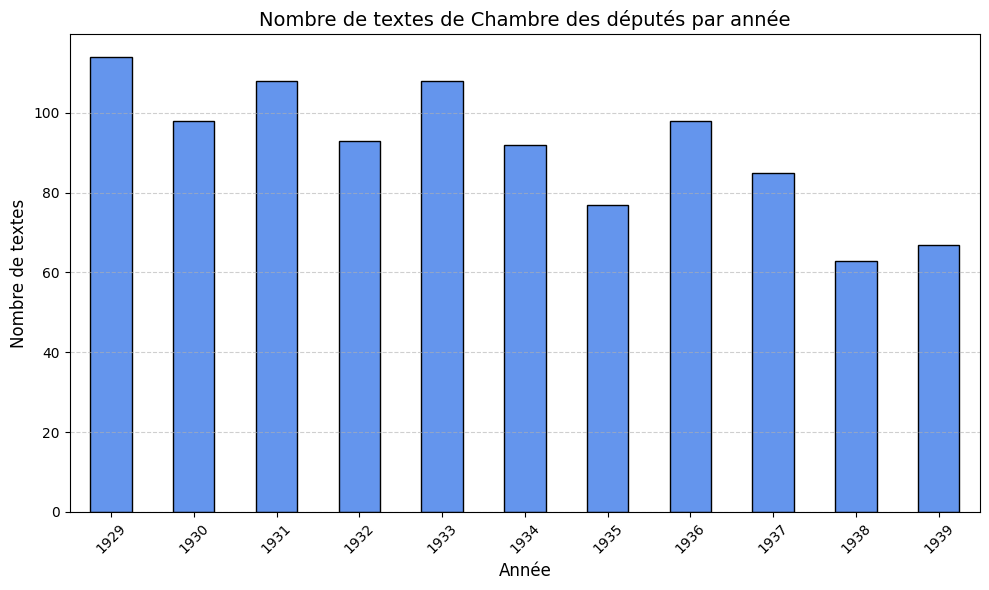
\includegraphics[width=0.75\textwidth]{img/dc.png}
\caption{Nombre de textes de Chambre des députés par année}
\end{figure}

En ce qui concerne la Chambre des députés, nous constatons qu'entre 1929 et 1939, le nombre annuel de comptes rendus de débats suit une tendance légèrement décroissante. Cette diminution est particulièrement marquée en 1938 et 1939, où le nombre de textes publiés représente environ la moitié de celui de 1929. Cela suggère qu'au cours de cette période, le nombre de séances tenues par la Chambre a progressivement diminué.

\begin{figure}
\centering %
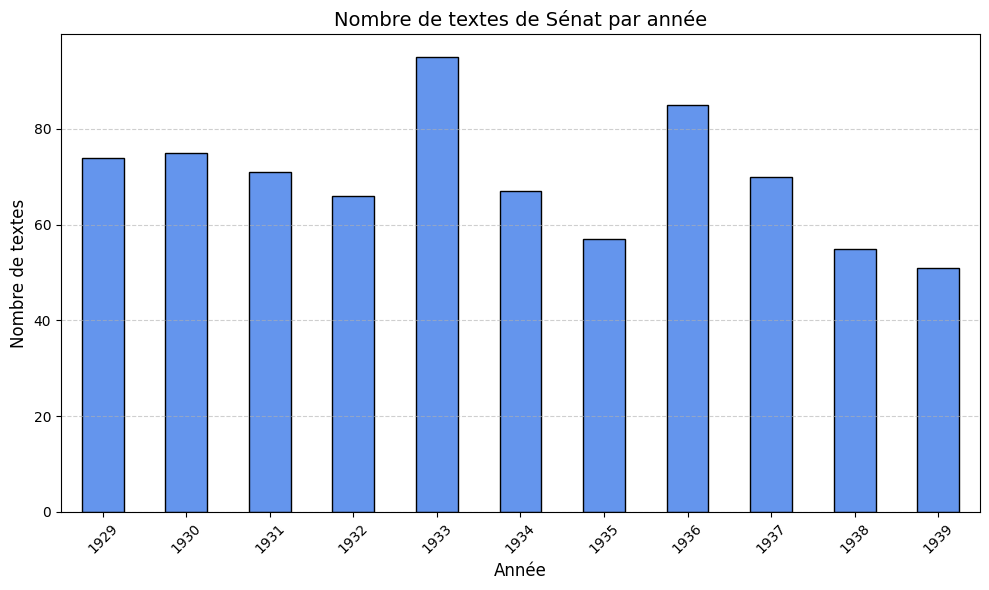
\includegraphics[width=0.75\textwidth]{img/ds.png}
\caption{Nombre de textes de Sénat par année}
\end{figure}

Du côté du Sénat, le nombre total de comptes rendus est inférieur à celui de la Chambre. De plus, la tendance générale de variation de ces rapports diffère quelque peu de celle observée à la Chambre. Bien qu'une légère baisse soit également perceptible en 1938 et 1939, les pics de production de comptes rendus au Sénat se situent en 1933 et en 1936, contrairement à ceux de la Chambre qui se concentrent principalement entre 1929 et 1931.

Sur le plan du contenu textuel, il n'existe pas de différence essentielle entre la Chambre des députés et le Sénat : dans les deux cas, il s'agit de transcriptions des interventions prononcées lors des séances. Chaque paragraphe correspond à une prise de parole individuelle, avec le nom ou la fonction de l'intervenant mis en gras, suivi de son discours. Sur cette base, les différents sujets abordés sont organisés selon l'ordre de la discussion pendant la séance, et sont introduits par une mention du thème concerné, par exemple "agriculture" ou "santé publique". En dehors de cela, la composition de chaque compte rendu peut varier en fonction du contenu spécifique de la séance, mais elle comporte généralement les sections suivantes : un sommaire, les absences et demandes de congé des participants, le procès-verbal, le texte intégral des articles de loi débattus, ainsi que des données chiffrées ou tableaux en lien avec les discussions. Dans la figure 3.3, on peut voir un scan d'un document issu de la séance de la Chambre des députés du 29 juin 1937.

\begin{figure}
\centering %
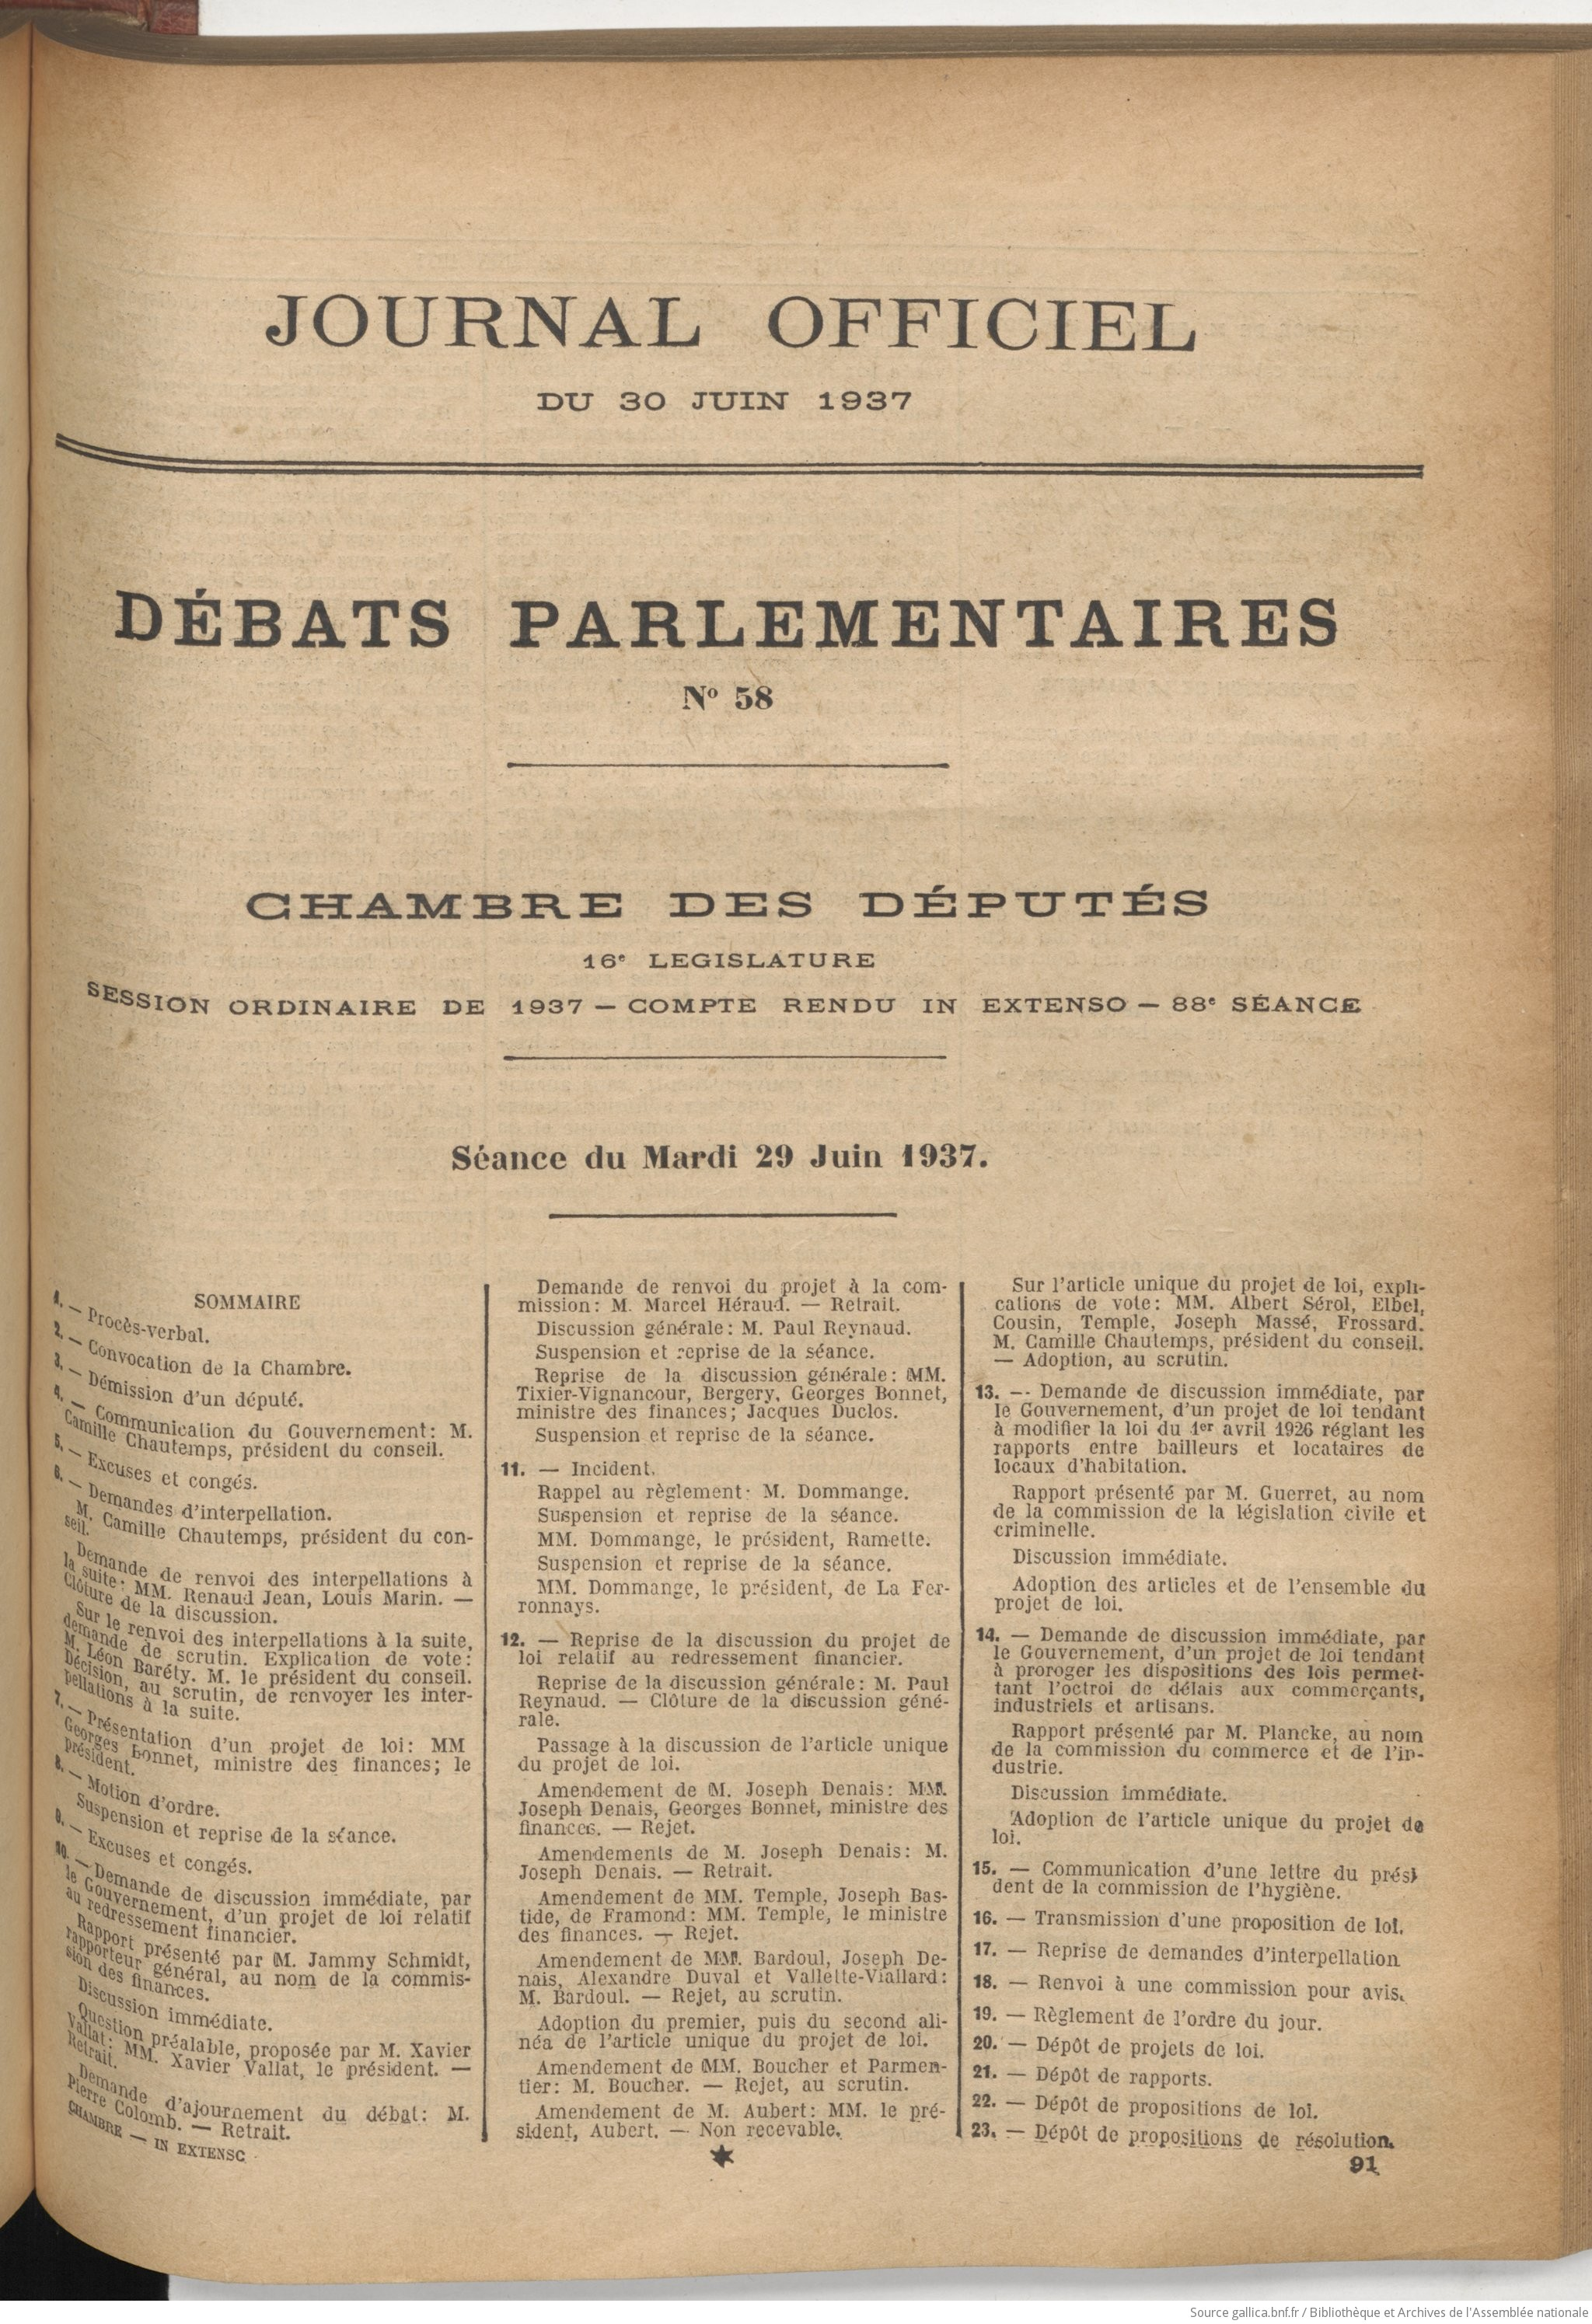
\includegraphics[width=0.75\textwidth]{img/exp.jpeg}
\caption{La première page de compte rendu de la séance du 29 juin 1937 de Chambre des députés}
\end{figure}

Il convient toutefois de souligner un point important : bien que nous ayons construit une base de données relativement complète, celle-ci contient encore un nombre non négligeable d'erreurs liées à la reconnaissance optique de caractères (OCR). Ces erreurs ne sont pas dues à une faible précision du modèle OCR lui-même, comme le montre l'exemple présenté dans la figure 3.4.

Dans cette figure, on voit à gauche une image numérisée du Journal officiel et, à droite, le texte OCR correspondant. Ce dernier apparaît largement illisible, presque sous forme de "charabia". Cette situation s'explique par une déformation des pages lors du processus de numérisation : certaines parties du texte sont alors complètement perdues, et il devient très difficile, voire impossible, de les récupérer même avec des méthodes de correction a posteriori.

Nous avons donc mené une analyse plus approfondie de la répartition de ces erreurs dans notre corpus afin d'évaluer leur poids relatif. Pour ce faire, nous avons utilisé le modèle fr\_core\_news\_sm de SpaCy\footcite{spacy2} pour effectuer la tokenisation de tous les textes. Ensuite, nous avons filtré les tokens répondant aux critères suivants : tokens uniques contenant plus de 15 caractères ; tokens comportant des caractères non standards pour le français ; tokens ne composés que partiellement de lettres alphabétiques. Bien que ces critères soient relativement grossiers, ils permettent néanmoins de dresser un aperçu général de la distribution des erreurs.

Par la suite, nous avons normalisé la longueur totale des textes, ce qui nous permet d'exprimer la position relative d'un segment donné en pourcentage. Nous avons alors comptabilisé la position des tokens filtrés dans le texte, ainsi que la proportion d'erreurs dans chaque segment représentant 1 \% de la longueur du texte. Les résultats de cette visualisation sont présentés dans les figures 3.4 et 3.5.



\begin{figure}
\centering %
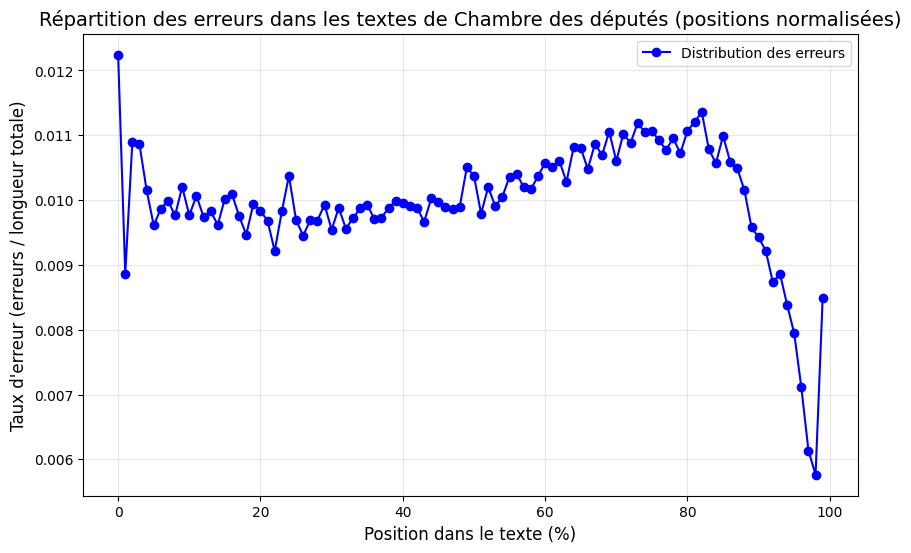
\includegraphics[width=0.75\textwidth]{img/ec.png}
\caption{Répartition des erreurs dans les textes de Chambre des députés (positions normalisées)}
\end{figure}

Les calculs révèlent que les textes de la Chambre des députés présentent un taux moyen d'erreurs de 13.35 \%. Il convient de préciser que le taux réel est probablement plus bas, car nous avons volontairement exclu les chiffres et les signes de ponctuation de nos critères de filtrage afin d'assurer une meilleure représentativité. La courbe de la figure 3.4 montre que les erreurs se concentrent principalement au début des textes. Cela est logique : dans les publications physiques, chaque compte rendu de séance commence généralement sur une page de droite, ce qui entraîne souvent une courbure du côté intérieur de la page lors du scan. Ensuite, on observe une légère hausse du taux d'erreur au fil du texte, qui reste toutefois relativement stable, avant de chuter brusquement à la fin.


\begin{figure}
\centering %
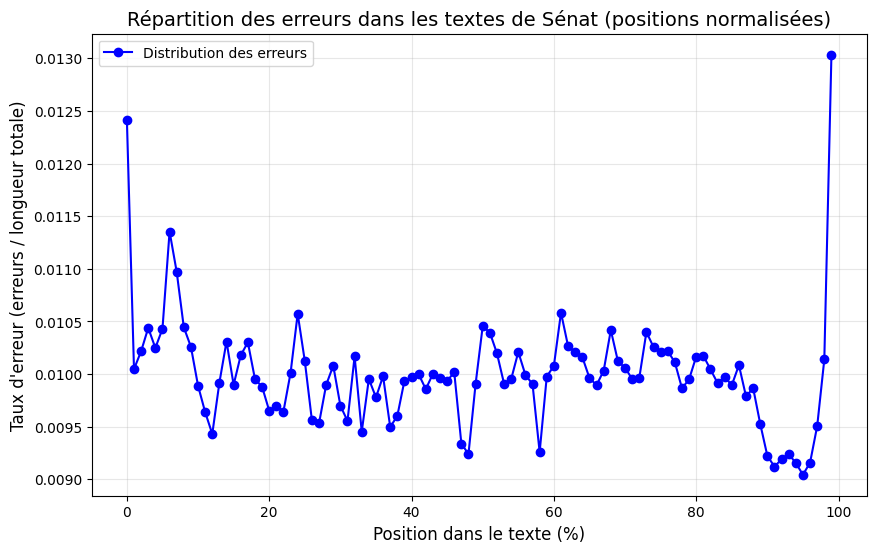
\includegraphics[width=0.75\textwidth]{img/es.png}
\caption{Répartition des erreurs dans les textes de Sénat (positions normalisées)}
\end{figure}

Les textes du Sénat présentent un taux moyen d'erreurs de 13.16 \%, ce qui est très proche de celui de la Chambre des députés. Cela semble indiquer que les deux sous-corpus sont confrontés à des problèmes similaires, et corrobore d'une certaine manière la fiabilité de notre méthode de détection d'erreurs. Toutefois, contrairement à la Chambre, les erreurs dans les textes du Sénat sont davantage concentrées au début et à la fin, et moins nombreuses au centre, avec une distribution légèrement plus irrégulière.

Quoi qu'il en soit, un taux d'erreurs avoisinant les 13 \% reste un chiffre significatif. Cela représente un véritable défi pour les traitements ultérieurs des données, et limite en partie la portée et la fiabilité de nos analyses. Nous reviendrons sur ce point dans la section suivante.


\section{Traitement des données}

Dans cette section, nous allons discuter de la manière dont nous traitons et analysons les données afin d'obtenir les résultats souhaités.

\subsection{Objectifs et étapes du pipeline de traitement}
Le premier défi lié au traitement des données réside dans l'indexation du système RAG, un processus particulièrement long et coûteux. Son objectif est de convertir une base de données externe en un format interrogeable rapidement par un LLM. Cependant, nos ressources computationnelles étant très limitées, nous avons suivi l'approche proposée par Silvestre de Sacy et al.\footcite{silvestredesacy2024}, en effectuant un filtrage préalable des données dès la phase amont afin de réduire la charge de travail pendant l'indexation.

Par conséquent, l'objectif préliminaire de notre traitement des données est de pouvoir extraire automatiquement, à partir du corpus, les textes liés à la politique internationale pour les analyser ultérieurement. La première étape consiste à corriger les erreurs présentes dans le corpus. Notre idée initiale était d'utiliser un modèle de langage pour effectuer une correction postérieure (post-correction) des textes, et nous avons effectué plusieurs essais en ce sens, sans toutefois obtenir de résultats satisfaisants, nous aborderons ce point plus en détail dans la section suivante.

Nous avons donc choisi comme première étape d'extraire les entités nommées à l'aide d'un modèle NER. Les modèles NER classiques sont généralement limités par les catégories d'entités nommées définies lors de leur pré-entraînement, et peuvent montrer des performances faibles sur des données ou des langues qu'ils n'ont pas rencontrées pendant cette phase. C'est pourquoi, dans notre pipeline de traitement des données, nous avons opté pour l'utilisation de GLiNER. GLiNER est un modèle NER basé sur une architecture d'encodeur transformeur bidirectionnel. Son avantage principal est qu'il permet aux utilisateurs de définir eux-mêmes les catégories d'entités nommées à détecter. Il présente également une bonne capacité de généralisation, est plus léger que d'autres modèles, et montre de meilleures performances en zero-shot dans diverses tâches de reconnaissance d'entités nommées par rapport à de grands modèles de langage comme ChatGPT\footcite{zaratiana2023}.

Dans notre processus, nous avons d'abord segmenté le texte complet en phrases à l'aide de la librairie NLTK\footcite{bird2004}, puis nous avons fusionné chaque tranche de trente phrases pour former un chunk. Afin de préserver la cohérence contextuelle, nous avons appliqué un chevauchement de cinq phrases entre les chunks. Ensuite, nous avons utilisé le modèle knowledgator/gliner-multitask-v1.0\footcite{2024d} pour traiter ces textes, en définissant les catégories d'entités suivantes (en anglais): "person", "country", "organization", "region".

À l'issue de cette étape, nous avons obtenu un dictionnaire contenant les entités nommées extraites à l'intérieur de chaque chunk. L'étape suivante consiste à filtrer les entités que nous considérons comme liées à la politique internationale. Pour ce faire, nous avons élaboré deux listes de référence : la première contient les noms de tous les pays existant entre 1929 et 1939 ; la seconde regroupe les noms et variantes des personnes ayant occupé le poste de ministre des Affaires étrangères en France pendant cette période.

Nous avons ensuite procédé à un double filtrage. La première étape consiste à calculer la distance de Levenshtein entre chaque entité extraite et les éléments des listes de référence. La distance de Levenshtein correspond au nombre minimal d'opérations (insertion, suppression, substitution) nécessaires pour transformer une chaîne de caractères en une autre\footcite{levenshteyn}. Par exemple, la distance entre cat et hat est de 1, tandis que celle entre cat et mad est de 2. Nous avons ensuite converti cette distance en pourcentage de similarité à l'aide d'une formule spécifique, qui est présentée comme suivant\footcite{zotero-734}. Afin d'éviter un filtrage excessif, nous avons fixé un seuil de similarité à 60\%.

\[
\text{similarité} = \left(1 - \frac{\text{distance de Levenshtein}(A, B)}{\max(\text{longueur}(A), \text{longueur}(B))} \right) \times 100
\]


Dans un second temps, nous avons effectué un filtrage plus fin à l'aide du modèle all-MiniLM-L6-v2\footcite{2024e}, qui permet de calculer la distance cosinus entre les entités filtrées et les éléments des listes de référence. Pour chaque entité, nous avons retenu la similarité maximale obtenue ; si ce score est supérieur à 0.8, nous considérons que l'entité est une variante ou une forme alternative d'un élément de la liste de référence, et nous la conservons.

Après avoir filtré les entités, nous obtenons un dictionnaire associant chaque entité à l'index du chunk dans lequel elle apparaît. On peut considérer que ces chunks sont susceptibles de concerner notre sujet d'intérêt, à savoir la politique internationale. Afin d'enrichir le contexte, nous avons fusionné chaque chunk avec ses voisins immédiats (le précédent et le suivant), ce qui nous a permis d'élargir l'information contextuelle. Au total, nous avons ainsi obtenu 58,136 chunks. Compte tenu de cette quantité, une annotation manuelle était irréaliste. Par ailleurs, définir ce qu'est exactement la "politique internationale" constitue un autre défi. Certains textes abordent de façon implicite des thématiques internationales, comme par exemple un texte sur l'agriculture qui peut en réalité évoquer des enjeux géopolitiques. En prenant en compte ces difficultés, nous avons choisi de recourir à un LLM pour déterminer automatiquement la pertinence de chaque texte.

Afin de maximiser la cohérence, nous avons simplifié notre définition de la politique internationale, que nous avons limitée aux relations entre la France et d'autres pays, ainsi qu'aux événements politiques se déroulant en dehors du territoire français. Sur cette base, nous avons extrait aléatoirement 8 000 chunks pour les soumettre à annotation automatique.

Notre premier choix de modèle était Deepseek-R1\footcite{deepseek-ai2025}, mais des limitations importantes du serveur ont conduit à des temps de réponse trop longs. Nous avons donc opté pour le modèle mistral-small-latest\footcite{zotero-743}, qui offrait un meilleur compromis entre vitesse et performance. Le prompt utilisé est le suivant (en français):

\begin{quote}
\small
\texttt{Veuillez déterminer si le texte suivant traite des relations entre la France et d'autres pays, ou d'événements spécifiques de la politique internationale en dehors de la France. Veuillez juger avec rigueur.\\
Si c'est le cas, retournez 1 ; sinon, ou si le texte ne fait que mentionner des noms liés, retournez 0.\\
Vous devez strictement respecter le format requis : vous ne pouvez répondre que par 0 ou 1, rien d'autre.\\
Texte : \{text\}\\
Votre réponse (uniquement 0 ou 1) :}
\end{quote}

Si le modèle estime que le texte est pertinent, il retourne "1" ; sinon, "0".

Sur la base des résultats de cette annotation, nous avons construit un classificateur combinant TF-IDF et régression logistique. Le TF-IDF permet de pondérer l'importance d'un terme en fonction de sa fréquence dans un document donné et de sa rareté dans l'ensemble du corpus\footcite{ramos2003}. La régression logistique utilise ensuite ces représentations pour effectuer la classification. Lors de l'entraînement, nous avons utilisé une recherche par grille pour optimiser les paramètres. Les meilleurs paramètres obtenus sont les suivants :\{C: 5.0, penalty: 'elasticnet', l1\_ratio: 0.8, tol: 0.001, fit\_intercept: False, class\_weight: None\}.





\begin{table}[ht]
\centering
\begin{tabular}{lcccc}
\hline
Classe & Précision & Rappel & Score F1 & Effectif \\
\hline
0 (Non-pertinent) & 0.93 & 0.97 & 0.95 & 1335 \\
1 (Pertinent)     & 0.80 & 0.65 & 0.71 & 265 \\
\hline
\textbf{Exactitude} & \multicolumn{3}{c}{\textbf{0.91}} & 1600 \\
\textbf{Moyenne macro} & 0.86 & 0.81 & 0.83 & 1600 \\
\textbf{Moyenne pondérée} & 0.91 & 0.91 & 0.91 & 1600 \\
\hline
\end{tabular}
\caption{Rapport de classification sur l'ensemble de test (exactitude = 0.9137)}
\label{tab:classification_report}
\end{table}

Les résultats du modèle sont globalement satisfaisants, comme celui montré dans la table 3.1, avec une précision de 91.4 \%. Pour la classe non pertinente (classe 0), la précision et le rappel atteignent respectivement 0.93 et 0.97, avec un F1-score de 0.95. Cela montre que le modèle identifie bien les textes hors du champ de la politique internationale. En revanche, pour la classe pertinente (classe 1), le rappel est plus faible (0.65), ce qui signifie que certains textes pertinents n'ont pas été détectés. Le F1-score y est de 0.71. La macro-moyenne du F1 est de 0.83, légèrement inférieure à la moyenne pondérée (0.91), ce qui révèle un déséquilibre dans la performance du modèle entre les deux classes.

\begin{table}[ht]
\centering
\begin{tabular}{ll@{\hskip 1cm}ll}
\textbf{Caractéristiques positives} & \textbf{Score} & \textbf{Caractéristiques négatives} & \textbf{Score} \\
\hline
\texttt{français} & 9.5053 & \texttt{colomb} & -10.7510 \\
\texttt{la france} & 9.2536 & \texttt{indre} & -9.9037 \\
\texttt{france} & 8.0773 & \texttt{rené} & -9.5429 \\
\texttt{franco} & 7.6649 & \texttt{seine} & -8.5810 \\
\texttt{espagne} & 7.4144 & \texttt{tardieu} & -8.2637 \\
\texttt{etats unis} & 7.0916 & \texttt{paul} & -6.7301 \\
\texttt{armements} & 6.8432 & \texttt{edouard} & -6.0142 \\
\texttt{allemagne} & 6.7793 & \texttt{pierre} & -5.9858 \\
\texttt{nations} & 6.7696 & \texttt{thomas} & -5.5364 \\
\texttt{angleterre} & 6.2520 & \texttt{œuvre} & -5.2522 \\
\texttt{italie} & 6.1476 & \texttt{loire} & -4.9609 \\
\texttt{genève} & 6.0317 & \texttt{iln} & -4.8065 \\
\texttt{accords} & 5.9966 & \texttt{albert} & -4.6377 \\
\texttt{approbation} & 5.8994 & \texttt{départements} & -4.5711 \\
\texttt{europe} & 5.7699 & \texttt{poincaré} & -4.5497 \\
\texttt{pays} & 5.4888 & \texttt{daladier} & -4.3899 \\
\texttt{du traité} & 5.4022 & \texttt{cher} & -4.3845 \\
\texttt{peuples} & 5.3557 & \texttt{travail} & -4.1955 \\
\texttt{allemandes} & 5.3174 & \texttt{andré} & -4.1699 \\
\texttt{traité} & 5.0717 & \texttt{maurice} & -4.1611 \\
\end{tabular}
\caption{Caractéristiques discriminantes identifiées par le classifieur}
\label{tab:features_table}
\end{table}

Dans la table 3.2, nous présentons les 20 caractéristiques les plus fortement associées à chaque classe. Du côté des textes liés à la politique internationale, on retrouve logiquement des mots comme "français", "la france", mais aussi de nombreux noms de pays : "espagne", "états unis", "allemagne", "angleterre", etc. Figurent aussi des termes relatifs à des organisations internationales ou à la diplomatie, comme "genève", "nations", "traité", "accords". Cela confirme que le classificateur capte bien des contenus représentatifs de notre sujet cible.

Pour la classe non pertinente, on remarque la présence importante de noms de personnalités politiques françaises comme "tardieu", "poincaré" ou "daladier", qui ont souvent exercé des fonctions internes. Ces noms apparaissent fréquemment dans de nombreux contextes, ce qui peut expliquer pourquoi le classificateur ne les associe pas fortement à des contenus internationaux. On trouve aussi des termes géographiques français comme "loire" ou "départements", généralement liés à des problématiques internes. Ces éléments renforcent la validité des décisions du modèle.

Nous avons ensuite appliqué le classificateur à l'ensemble du corpus. Deux approches avaient initialement été envisagées : soit inclure le document complet contenant chaque chunk pertinent, soit élargir artificiellement le contexte par ajout des chunks voisins. Ces deux méthodes ont cependant fortement rallongé le temps d'indexation. Nous avons donc choisi de ne conserver que les chunks pertinents eux-mêmes. Au final, nous avons extrait 8,623 chunks du corpus de la Chambre des députés et 2,678 chunks du corpus du Sénat.

Les étapes suivantes consistent à indexer ces textes afin que les LLMs puissent ensuite les interroger directement. Après avoir testé plusieurs solutions différentes, en tenant compte de la vitesse de traitement, des performances réelles et de la compatibilité avec divers modèles et plateformes, nous avons finalement choisi la solution LightRAG\footcite{guo2024}. Nous avons utilisé Llama3.1:8b\footcite{zotero-754}, fourni par Ollama, comme modèle de base, et nomic-embed-text\footcite{zotero-756} comme modèle d'embedding.L'ensemble du processus d'indexation a été effectué sur une carte RTX 4090, et a duré au total plus de soixante heures. Le résultat final est un graphe de connaissances contenant les informations clés du corpus, ainsi que d'autres éléments destinés à aider à la génération des réponses. À partir des textes de la Chambre des députés, nous avons obtenu un graphe de réseau avec 40,474 nœuds et 23,426 arêtes, tandis que pour le Sénat, nous avons obtenu un graphe avec 17,964 nœuds et 11,084 arêtes.



Le résultat final est une base de connaissances structurée sous forme de graphe, contenant les informations les plus pertinentes du corpus et destinée à être interrogée par un modèle de génération.

Il convient néanmoins de souligner que la qualité des réponses générées dans un système RAG dépend fortement des capacités du modèle de langage utilisé. Le modèle Llama 3.1:8B, bien que performant, présente parfois des hallucinations notables. Pour contourner cette limitation, nous avons intégré Gemini-CLI\footcite{2025a}, un outil développé par Google permettant d'utiliser leurs modèles depuis un terminal. Il prend en charge la lecture de fichiers locaux, ce qui permet un fonctionnement proche de celui de LightRAG, mais avec une capacité de génération nettement améliorée. Le pipeline complet est illustré dans la figure 3.6.

\begin{figure}
\centering %
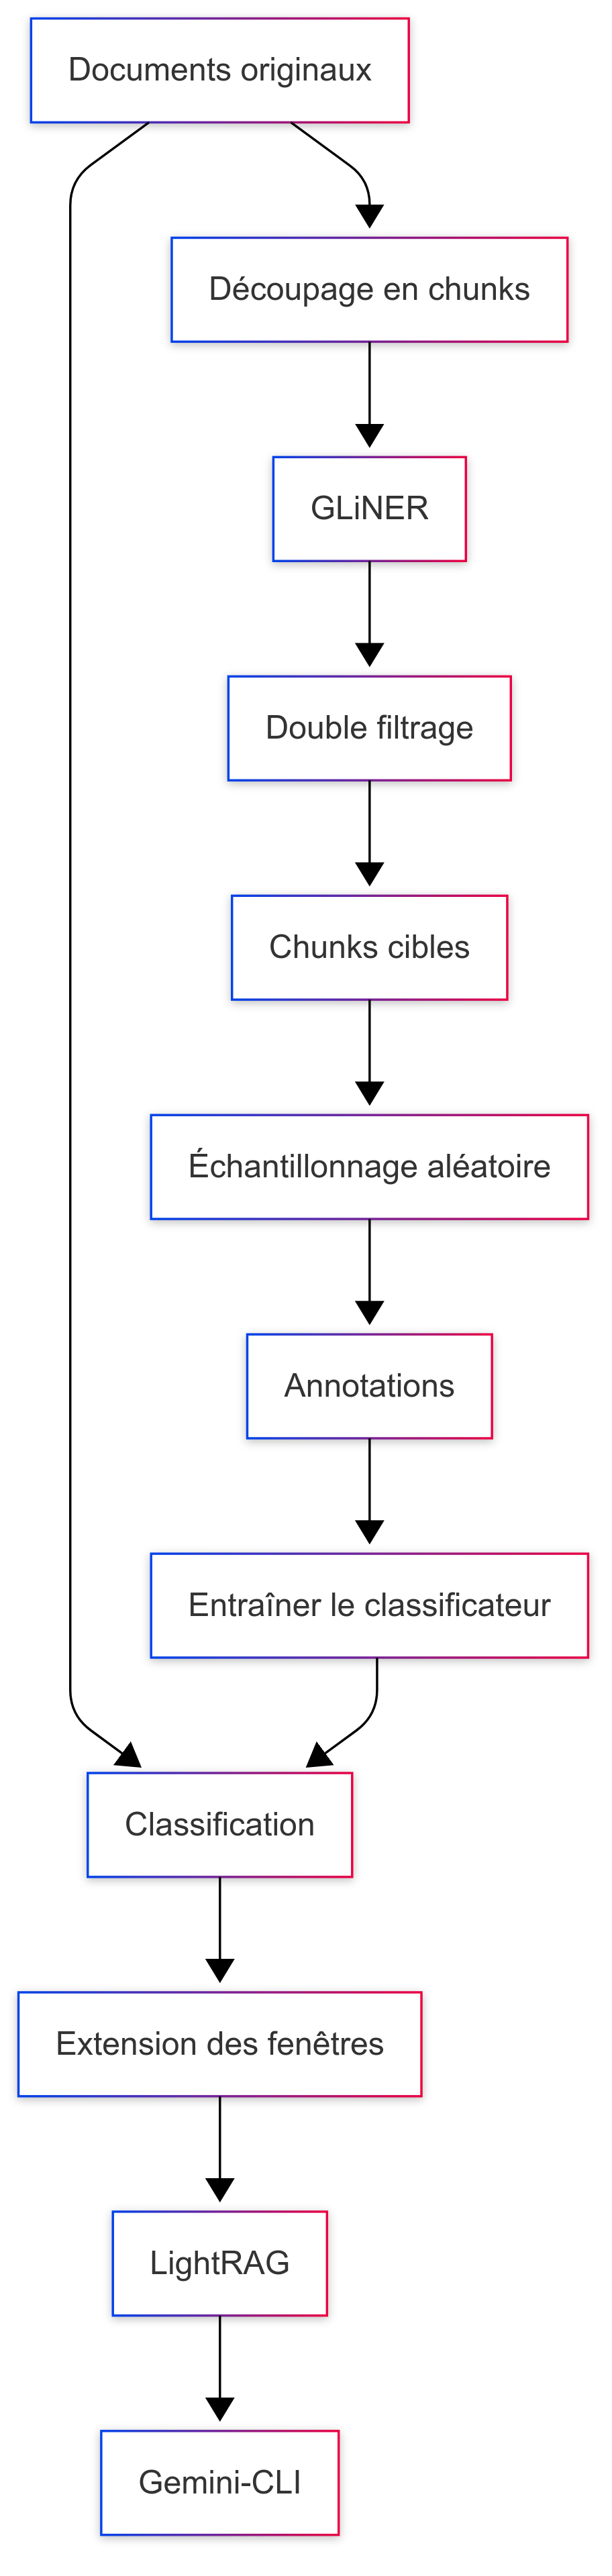
\includegraphics[width=\textwidth,height=0.9\textheight,keepaspectratio]{img/pipeline.png}
\caption{Vue générale du pipeline}
\end{figure}

Pour évaluer les performances d'un système RAG en matière de questions-réponses, une méthode générale de base consiste à construire un jeu de données de référence (“golden dataset”) avec des paires questions-réponses, puis à comparer les réponses générées par le RAG avec les réponses correctes\footcite{zotero-749}. Sur cette base, il existe également des métriques d'évaluation plus fines et plus détaillées\footcite{yu2025}. Cependant, en raison de la portée limitée et des ressources restreintes de cette étude, nous ne sommes pas en mesure de réaliser une évaluation complète basée sur les méthodes mentionnées ci-dessus. Nous avons donc opté pour une approche plus simple et intuitive : demander au RAG de répondre à trois questions dont nous connaissons déjà les réponses, en se basant sur le graphe de connaissances, puis vérifier manuellement l'exactitude de ses réponses.

Les questions posées, ainsi que les réponses du système RAG, sont les suivantes (en anglais) :

\begin{quote}
\textbf{1.} \textit{According to the document, when did the Yen Bay uprising occur?} \\
\textbf{Réponse:} According to the document, the Yen Bay uprising occurred on February 12, 1930.

\vspace{1em}

\textbf{2.} \textit{According to the document, which countries are involved in the Munich Agreement?} \\
\textbf{Réponse:} Based on the document, the countries involved in the Munich Agreement were:
\begin{itemize}
  \item Germany
  \item France
  \item Great Britain
  \item Italy
\end{itemize}
Czechoslovakia was the country whose territory was ceded as a result of the agreement. Other countries mentioned in the context of the agreement include Poland, Hungary, and the Soviet Union.

\vspace{1em}

\textbf{3.} \textit{According to the document, which are the member countries of the Stresa Front?} \\
\textbf{Réponse:} According to the document, the member countries of the Stresa Front were France, Britain, and Italy.
\end{quote}


En analysant ces réponses, on constate que le système RAG a été capable de retrouver avec succès les informations demandées dans les données et de les résumer de manière cohérente. La seule erreur concerne la première question : l'insurrection de Yên Bái a en réalité eu lieu le 10 février 1930. Cependant, étant donné que les conséquences de cet événement se sont étendues sur plusieurs mois, cette erreur semble provenir du contenu même du texte, plutôt que du processus de récupération d'information. Ainsi, nous pouvons considérer que la bonne performance du système RAG dans la recherche d'informations constitue une base solide pour les analyses ultérieures.

\subsection{Problèmes rencontrés et limites méthodologiques}

Notre pipeline de traitement des données satisfait globalement à nos exigences, mais présente encore un certain nombre de lacunes.

Tout d'abord, du côté des données, les textes que nous traitons contiennent inévitablement une quantité non négligeable d'erreurs d'OCR. Nous avons tenté plusieurs méthodes de post-correction de ces erreurs. L'une des approches les plus représentatives repose sur les comptes rendus des séances publiques du Sénat, disponibles depuis 2003\footcite{zotero-758}. En échantillonnant les types d'erreurs présents dans nos données, nous avons injecté aléatoirement du bruit dans les textes corrects pour simuler les erreurs d'OCR que nous rencontrons. Ce jeu de données est disponible sur Huggingface\footcite{2025b}. Ensuite, en nous inspirant des travaux de Thomas et al.\footcite{thomas2024}, nous avons entraîné un modèle de correction basé sur BART\footcite{2025c}. Cependant, les résultats finaux ont été décevants. Par conséquent, l'amélioration de la qualité des textes OCR reste une priorité essentielle pour obtenir de meilleurs résultats.

Deuxièmement, la limitation de nos ressources de calcul constitue également un défi. L'approche RAG pré-ciblé, bien qu'elle nous permette de réduire considérablement le temps de traitement des données, restreint fortement notre champ d'exploration lors de l'analyse. Ainsi, la méthode la plus idéale consisterait toujours à traiter l'intégralité du corpus et à réaliser des interactions de type questions-réponses. Cependant, il est encore plus important de trouver un équilibre entre le coût computationnel et la qualité des résultats obtenus. Nous reviendrons de manière plus détaillée sur ce point dans la conclusion.

Troisièmement, lors de l'étape d'extraction des caractéristiques textuelles par TF-IDF, le déséquilibre entre le nombre des étiquettes des deux classes a limité la capacité du classificateur à identifier correctement les échantillons positifs. Cela implique potentiellement que certains textes liés à la politique internationale, mais dont les caractéristiques diffèrent de celles observées dans les textes existants, aient été écartés. En d'autres termes, notre classificateur présente dans une certaine mesure un biais. La situation idéale consisterait à annoter un ensemble plus large d'échantillons, puis à en extraire un nombre équilibré pour l'entraînement, ou encore à recourir à différentes méthodes d'échantillonnage et à des fonctions de perte adaptées. Toutefois, les contraintes financières et temporelles de cette recherche ne nous ont pas permis de mettre en œuvre ces solutions, ce qui constitue une limite regrettable.

Enfin, la complexité de notre pipeline limite l'intervention humaine, ce qui rend difficile le contrôle qualité à petite échelle. Même si les résultats finaux sont globalement satisfaisants, nous n'avons pas réellement procédé à une vérification manuelle de la qualité des annotations produites par le LLM, ni à un contrôle ni une amélioration du processus de formation des classificateurs. Sur ce point, la qualité des données obtenues pourrait être améliorée. Dans nos recherches futures, nous essaierons d'optimiser davantage notre processus, tant en termes de rapidité que d'efficacité.

\chapter{Résultats}

Dans ce chapitre, nous procéderons à l'analyse de notre corpus et tenterons de répondre aux questions de recherche formulées précédemment. Nous examinerons les résultats relatifs à la Chambre des députés et au Sénat à la fois dans une perspective macro et micro. D'un point de vue macro, nous chercherons à clarifier la structure fondamentale du graphe élaboré à partir du corpus. D'un point de vue micro, nous mènerons une investigation ciblée sur certains nœuds et contenus clés, afin de présenter les résultats de manière systématique.



\section{Chambre des députés}

\subsection{Analyse macrostructurelle}

\begin{figure}
\centering %
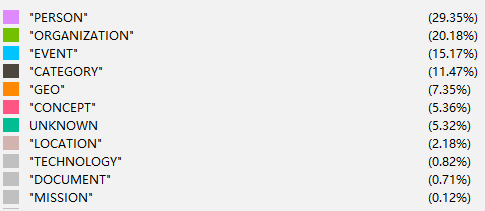
\includegraphics[width=0.75\textwidth]{img/chambre_entity_type.png}
\caption{Les types d'entités les plus représentés – Graphe de la Chambre des députés}
\end{figure}

Nous commencerons par analyser les données relatives à la Chambre. Dans la figure 4.1, nous pouvons observer que les sept catégories de nœuds les plus fréquentes représentent à elles seules 91.06 \% du total (sans inclure la catégorie UNKNOWN). Parmi elles, les catégories PERSON, ORGANIZATION et EVENT représentent à elles seules plus de la moitié. Ce point constitue un appui essentiel pour notre projet de réorganisation de l'information via des LLM afin de générer des réponses.




\begin{figure}
\centering %
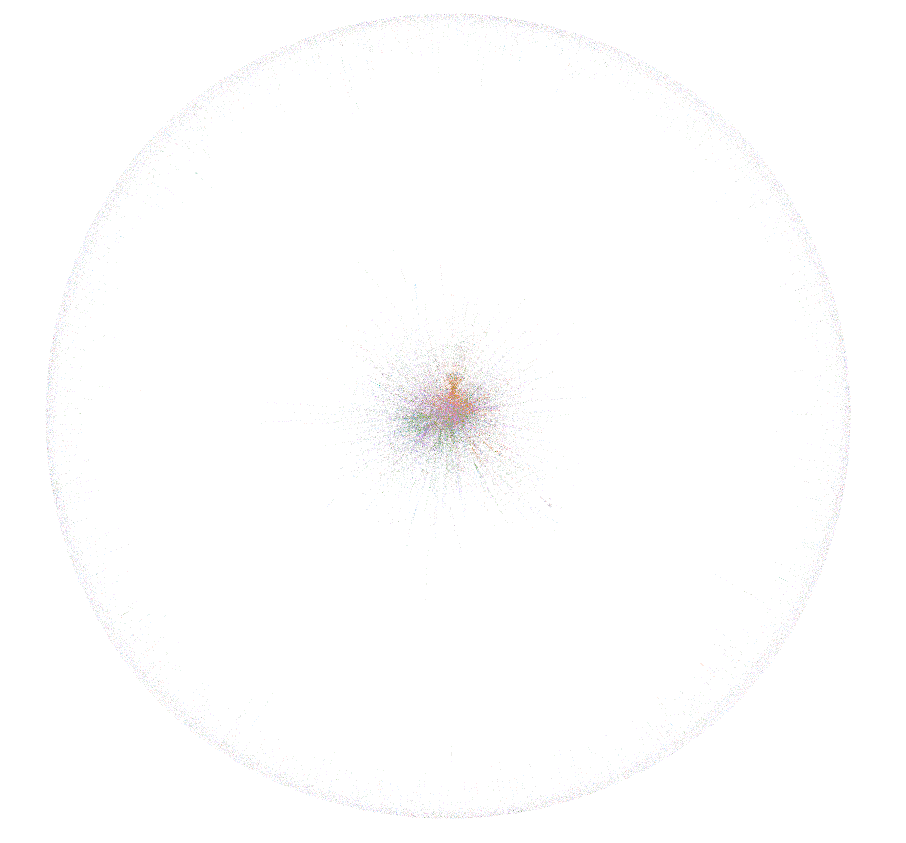
\includegraphics[width=0.75\textwidth]{img/chambre_general_view.png}
\caption{Vue générale – Graphe de la Chambre des députés}
\end{figure}

\begin{figure}
\centering %
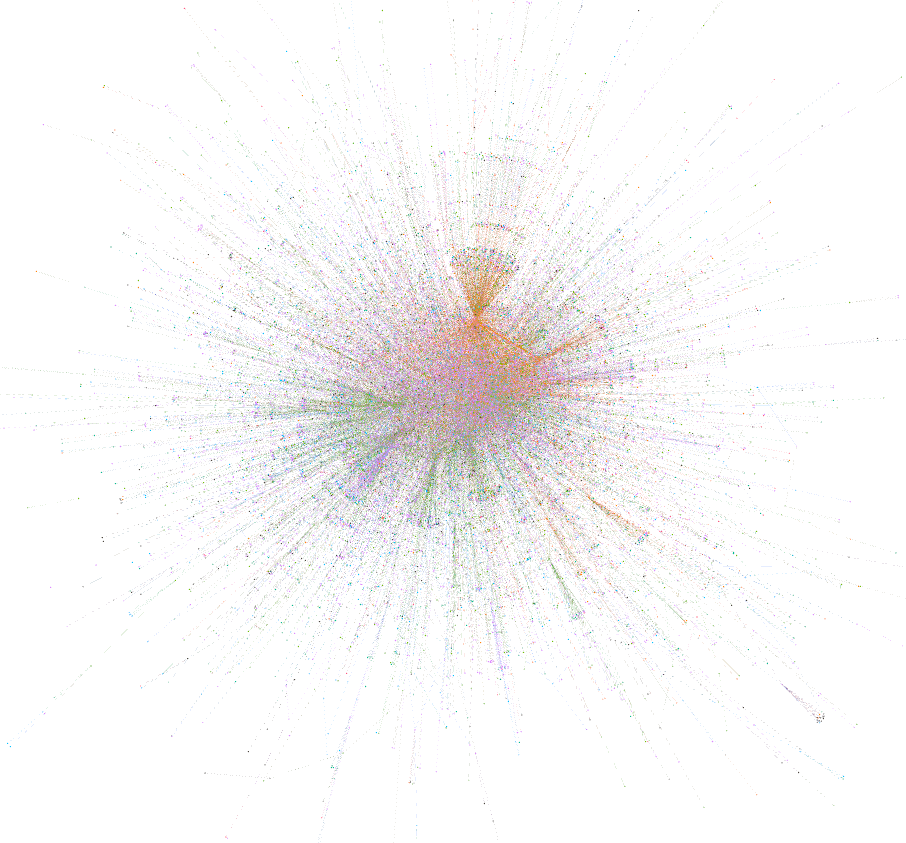
\includegraphics[width=0.75\textwidth]{img/chambre_close_view.png}
\caption{Centre du graphe – Graphe de la Chambre des députés}
\end{figure}

Par la suite, nous avons utilisé l'algorithme de visualisation proposé par Hu\footcite{hu2006} pour réajuster la disposition des nœuds et des arêtes dans le graphe de connaissances. Grâce à cet algorithme, comme le montre la figure 4.2, on remarque que dans le graphe de la Chambre, le nombre de nœuds dépasse celui des arêtes, ce qui signifie qu'un grand nombre de nœuds ne sont pas connectés. Grâce à l'algorithme, ces nœuds non connectés ont été relégués à la périphérie de l'image, tandis que les nœuds entretenant des relations complexes ont été regroupés au centre, comme illustré dans la figure 4.3. Nous avons calculé que le degré moyen de l'ensemble du réseau est de 1,158, et le degré pondéré moyen est de 14,293. Le premier chiffre indique que le réseau est globalement assez sparse, tandis que le second montre que, bien que le nombre de connexions soit faible, certaines arêtes portent un poids très élevé. Nous discuterons plus en détail de ce phénomène par la suite.

\begin{figure}
\centering %
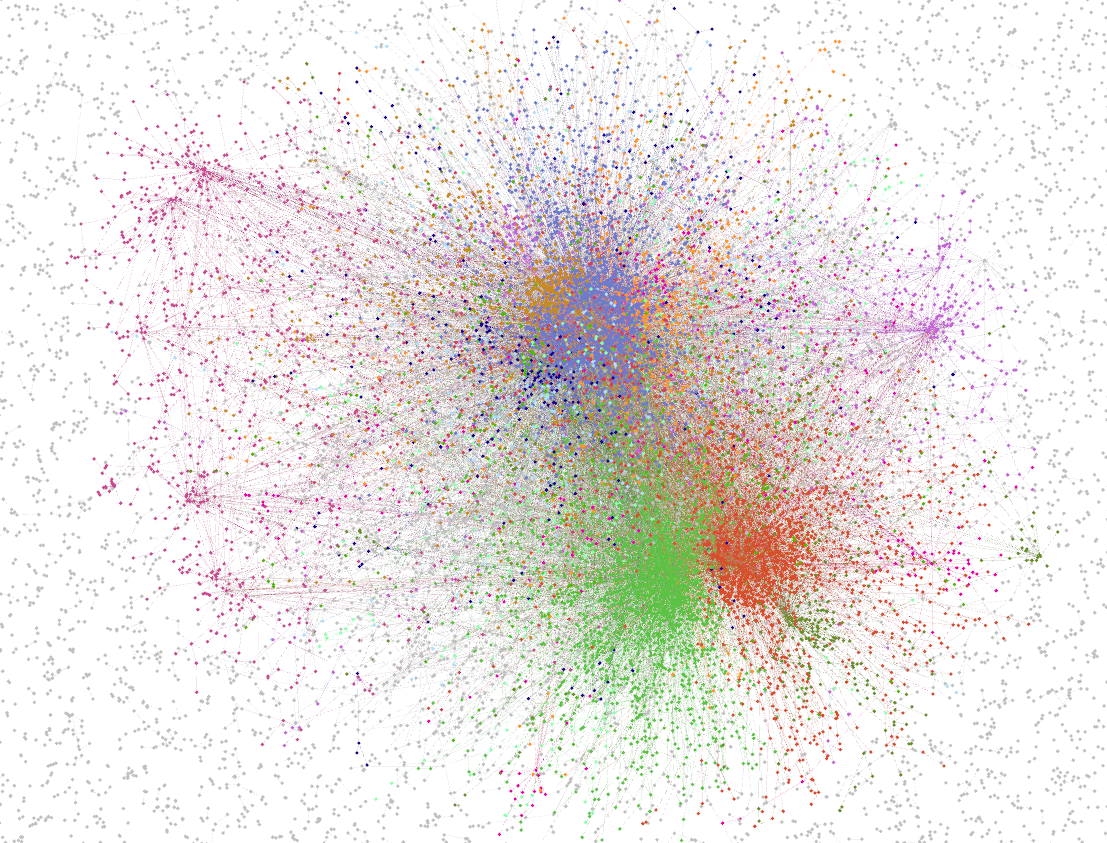
\includegraphics[width=0.75\textwidth]{img/chambre_openord.png}
\caption{La distribution des nœuds réorganisée par OpenORD – Graphe de la Chambre des députés}
\end{figure}

Sur cette base, nous avons utilisé l'algorithme Leiden\footcite{traag2019} pour explorer les communautés composées des nœuds centraux dans l'ensemble du graphe de connaissances. L'algorithme Leiden est une amélioration de l'algorithme Louvain\footcite{blondel2008} ; par rapport à ce dernier, il impose que toutes les communautés soient connectées, ce qui permet d'obtenir une qualité de regroupement significativement meilleure. Nous avons fixé le paramètre de resolution à 1, qui contrôle la taille et la finesse des communautés : plus la valeur est faible, plus les communautés seront grandes, et plus elle est élevée, plus le découpage sera fin. Une valeur de 1 correspond à une granularité moyenne. Après calcul, nous avons obtenu un score de modularité de 0.661, ce qui indique que les connexions à l'intérieur des communautés sont relativement denses et que la partition est pertinente. La distribution des nœuds est montrée dans la figure 4.5.

\begin{figure}
\centering %
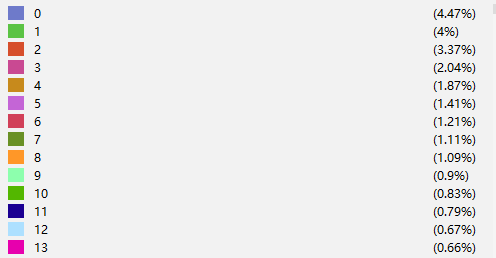
\includegraphics[width=0.75\textwidth]{img/chambre_cluster.png}
\caption{Proportion du nombre de nœuds par cluster – Graphe de la Chambre des députés}
\end{figure}

Les 40,747 nœuds du graphe de la Chambre ont ainsi été répartis en 23,426 communautés. Étant donné le grand nombre de nœuds isolés, ce résultat est logique. Comme le montre la figure 4.5, la plus grande communauté représente 4.47\% de l'ensemble des nœuds. On compte 9 communautés représentant chacune plus de 1 \% du total, et 14 communautés dépassant 0.5 \%. Nous avons choisi de colorer ces communautés et de les représenter à l'aide de l'algorithme OpenORD\footcite{martin2011}, qui est spécifiquement conçu pour traiter des structures de graphes de grande taille. Le résultat est présenté en figure 4.4.

\begin{table}[htbp]
\centering
\begin{tabular}{|c|p{12cm}|}
\hline
\textbf{Cluster} & \textbf{Nœuds représentatifs (par fréquence décroissante)} \\
\hline
0 & FRANCE (1494), ALLEMAGNE (319), GERMANY (147), ITALIE (121), ANGLETERRE (110) \\
1 & LA FRANCE (522), L'ALLEMAGNE (304), LA SOCIÉTÉ DES NATIONS (223), LE GOUVERNEMENT FRANÇAIS (136), L'ANGLETERRE (109) \\
2 & LE GOUVERNEMENT (412), LA CHAMBRE (366), M. LE PRÉSIDENT (328), M. LE PRÉSIDENT DU CONSEIL (218), LA CHAMBRE DES DÉPUTÉS (148) \\
3 & FRANCE (111), GOUVERNEMENT (80), LA FRANCE (63), LA CHAMBRE (44), M. LE PRÉSIDENT (39) \\
4 & GOUVERNEMENT (609), M. LE MINISTRE DU COMMERCE (73), PARLEMENT (58), COMMISSION DE L'AGRICULTURE (39), M. LE RAPPORTEUR (37) \\
5 & COMMISSION DES DOUANES ET DES CONVENTIONS COMMERCIALES (152), COMMISSION DES FINANCES (110), M. LE MINISTRE DES COLONIES (44), M. TAUDIÈRE (44), M. LE MINISTRE DU COMMERCE ET DE L'INDUSTRIE (33) \\
6 & SOCIÉTÉ DES NATIONS (278), GOUVERNEMENT FRANÇAIS (178), GENÈVE (69), BRIAND (45), M. BERGERY (33) \\
7 & CHAMBRE DES DÉPUTÉS (156), SÉNAT (89), PROPOSITION DE LOI (42), COMMISSION DE LA LÉGISLATION CIVILE ET CRIMINELLE (27), GASTON DOUMERGUE (23) \\
8 & HITLER (214), MUSSOLINI (79), FRANCO (41), LEAGUE OF NATIONS (33), GRUMBACH (29) \\
9 & INDOCHINE (50), MARIUS MOUTET (38), L'INDOCHINE (31), COLONIES (25), JACQUES DORIOT (22) \\
10 & PLAN YOUNG (102), M. HENRY FRANKLIN-BOUILLON (69), M. LOUIS MARIN (67), M. EDOUARD HERRIOT (58), BANQUE DES RÈGLEMENTS INTERNATIONAUX (44) \\
11 & LÉON BLUM (143), LOUIS MARIN (58), HENRY FRANKLIN-BOUILLON (48), PAUL REYNAUD (47), PAUL-BONCOUR (36) \\
12 & M. LE MINISTRE DES AFFAIRES ÉTRANGÈRES (189), COMMISSION DES AFFAIRES ÉTRANGÈRES (63), LA COMMISSION DES AFFAIRES ÉTRANGÈRES (36), EDOUARD HERRIOT (30), M. GUERNUT (14) \\
13 & M. LE MINISTRE DES FINANCES (92), M. LE MINISTRE DE L'AGRICULTURE (67), M. AMIDIEU DU CLOS (25), LE MINISTRE DE L'AGRICULTURE (24), LE MINISTRE DU COMMERCE (22) \\
\hline
\end{tabular}
\vspace{0.5em}  
\caption{Représentants les plus fréquents par cluster – Graphe de la Chambre des députés}
\label{tab:clusters-nœuds}
\end{table}

Nous avons effectué un décompte des cinq nœuds ayant le plus grand nombre d'arêtes dans chaque communauté, comme le montre le tableau 4.1. À partir de ces résultats, nous pouvons identifier les thèmes principaux suivants : les relations bilatérales ou multilatérales de la France avec d'autres pays (cluster 0) ; la diplomatie dans le cadre de la Société des Nations (cluster 1, cluster 6, cluster 8) ; les affaires des différents ministères gouvernementaux (cluster 4, cluster 5, cluster 12, cluster 13) ; les affaires parlementaires (cluster 2, cluster 3, cluster 7, cluster 11) ; les questions liées à l'après-Première Guerre mondiale (cluster 10) ; et les affaires coloniales (cluster 9). Nous pouvons en conclure que ces différenciations thématiques reflètent les axes principaux du contenu de notre corpus.

\begin{table}[ht]
\centering
\begin{tabular}{ll@{\hskip 1cm}ll}
\hline
\textbf{Étiquette du nœud} & \textbf{Nombre d'arêtes}  \\
\hline
\texttt{FRANCE} & 1494 \\
\texttt{GOUVERNEMENT} & 609 \\
\texttt{LA FRANCE} & 522 \\
\texttt{LE GOUVERNEMENT} & 412 \\
\texttt{LA CHAMBRE} & 366 \\
\texttt{M. LE PRÉSIDENT} & 328 \\
\texttt{ALLEMAGNE} & 319 \\
\texttt{L'ALLEMAGNE} & 304 \\
\texttt{SOCIÉTÉ DES NATIONS} & 238 \\
\texttt{LA SOCIÉTÉ DES NATIONS} & 223 \\
\texttt{M. LE PRÉSIDENT DU CONSEIL} & 218 \\
\texttt{HITLER} & 214 \\
\texttt{M. LE MINISTRE DES AFFAIRES ÉTRANGÈRE} & 189 \\
\texttt{GOUVERNEMENT FRANÇAIS} & 178 \\
\texttt{CHAMBRE DES DÉPUTÉS} & 156 \\
\texttt{COMMISSION DES DOUANES ET DES CONVENTIONS COMMERCIALES} & 152 \\
\texttt{LA CHAMBRE DES DÉPUTÉS} & 148 \\
\texttt{GERMANY} & 147 \\
\texttt{LÉON BLUM} & 143 \\
\texttt{CHAMBRE} & 132 \\
\texttt{LE GOUVERNEMENT FRANÇAIS} & 136 \\
\texttt{ITALIE} & 121 \\
\texttt{FRANCE} & 111 \\
\texttt{ANGLETERRE} & 111 \\
\texttt{COMMISSION DES FINANCE} & 110 \\
\texttt{L'ANGLETERRE} & 109 \\
\texttt{WASHINGTON} & 108 \\
\texttt{PLAN YOUNG} & 102 \\
\hline
\end{tabular}
\caption{Nœuds avec le plus grand nombre d'arêtes – Graphe de la Chambre des députés}
\label{tab:features_table}
\end{table}

Ensuite, nous avons identifié les nœuds ayant plus de cent connexions, ce qui indique que ces entités apparaissent fréquemment dans le corpus et qu'elles ont été dotées d'une certaine importance sémantique. Les résultats sont présentés dans le tableau 4.2.

On peut constater que ce tableau contient encore quelques erreurs mineures, telles que l'apparition du mot GERMANY en anglais, alors qu'après vérification manuelle, ce mot n'apparaît pas dans le texte source. Nous supposons que cette erreur provient d'un hallucination générée par le modèle Llama 3.1:8b lors de l'extraction des entités. Étant donné que ce modèle présente un taux d'hallucination de 5.1 \% selon le Hallucination Leaderboard\footcite{zotero-768}, ce phénomène n'est pas surprenant. Cela dit, l'impact sémantique reste relativement limité, et nous avons jugé cette erreur acceptable.

Par ailleurs, nous avons observé l'existence d'un certain nombre de nœuds sémantiquement redondants, tels que FRANCE et LA FRANCE. Ce phénomène provient toujours de l'étape d'extraction des entités nommées : certaines entités sont extraites avec leur article défini comme une seule unité, tandis que d'autres, bien qu'identiques, reçoivent un type différent. Nous estimons que cela reflète en partie le contexte spécifique, et avons donc choisi de ne pas les modifier ni les fusionner.

Sur cette base, on peut déjà dégager les principaux points d'intérêt du texte issu de la Chambre : notamment les pays voisins de la France, comme l'Allemagne, l'Italie et le Royaume-Uni, l'Allemagne étant la plus évoquée, ce que la présence de HITLER dans la liste vient confirmer. Ensuite, la Société des Nations attire aussi une attention notable au sein du parlement, suscitant de nombreuses discussions. Enfin, une partie du discours semble concerner les réparations d'après-guerre et les accords diplomatiques, avec des entités telles que COMMISSION DES DOUANES ET DES CONVENTIONS COMMERCIALES, le PLAN YOUNG, ou encore WASHINGTON.

\begin{table}[ht]
\centering
\begin{tabular}{ll@{\hskip 1cm}ll}
\hline
\textbf{Nœud source} & \textbf{Nœud cible} & \textbf{Poids} \\
\hline
FRANCE & ALLEMAGNE & 2186.0 \\
FRANCE & ITALIE & 1023.0 \\
FRANCE & ANGLETERRE & 960.0 \\
LA FRANCE & L'ALLEMAGNE & 905.0 \\
LA CHAMBRE & M. LE PRÉSIDENT & 901.0 \\
FRANCE & GERMANY & 897.0 \\
GOUVERNEMENT & FRANCE & 751.0 \\
FRANCE & SOCIÉTÉ DES NATIONS & 748.0 \\
ALEX & FIRST CONTACT & 489.0 \\
LA CHAMBRE & LE GOUVERNEMENT & 468.0 \\
CHAMBRE DES DÉPUTÉS & SÉNAT & 468.0 \\
SAM RIVERA & INTELLIGENCE & 424.0 \\
LA FRANCE & L'ANGLETERRE & 354.0 \\
FRANCE & ESPAGNE & 350.0 \\
ALLEMAGNE & HITLER & 339.0 \\
FRANCE & HITLER & 321.0 \\
FRANCE & EUROPE & 318.0 \\
\hline
\end{tabular}
\caption{Relations pondérées entre entités – Graphe de la Chambre des députés}
\label{tab:features_table}
\end{table}

D'un autre côté, nous avons également analysé les informations relatives aux arêtes, en listant dans le tableau 4.3 celles dont le poids dépasse 300. Ce poids représente le nombre de fois où la relation a été mentionnée dans le corpus original. Nous avons tout d'abord remarqué des contenus hallucinés, tels que ALEX et FIRST CONTACT, ou encore SAM RIVERA et INTELLIGENCE. Suite à notre enquête, nous avons constaté que cette situation est en réalité due à l'inclusion de ces contenus en tant qu'exemples dans le prompt envoyé par LightRAG au LLM\footcite{zotero-779}. Un autre exemple similaire sera présenté par la suite.

Mis à part cela, nous avons observé que l'arête entre FRANCE et ALLEMAGNE est la plus importante de tout le graphe, avec un poids de 2,186, soit plus du double du second. L'arête entre LA FRANCE et L'ALLEMAGNE atteint également un poids de 897, sans compter les autres nœuds représentant des variantes de l'Allemagne. Cela démontre l'importance cruciale des relations franco-allemandes dans les débats de la chambre à cette époque.

Ensuite, nous notons que les liens entre la France et le Royaume-Uni, l'Italie, et l'Espagne ont également des poids très élevés. Il est intéressant de remarquer que l'arête entre la France et la Société des Nations a un poids de 748, la classant en 8\textsuperscript{e} position. Celle entre la France et l'Europe atteint 318. Cela suggère que la diplomatie bilatérale ou multilatérale dans le cadre de la Société des Nations et au sein de l'Europe a été largement discutée dans la chambre.

Enfin, le point HITLER est un cas particulier : c'est le seul nœud représentant une personne parmi ceux associés à une arête de poids supérieur à 300. Cela confirme une fois de plus l'attention portée par la France à l'Allemagne.



\subsection{Analyse microstructurelle}

Comme nous l'avons mentionné dans les chapitres précédents, la pratique de la diplomatie multilatérale de cette période peut être grossièrement divisée en deux types : la première se déroulant dans le cadre de la Société des Nations, et la seconde fonctionnant en parallèle de ce cadre. Dans notre recherche, nous considérons davantage le multilatéralisme comme une forme institutionnalisée de la diplomatie multilatérale ; par conséquent, dans notre analyse, nous considérons la Société des Nations comme une preuve emblématique de l'existence du multilatéralisme.

Nous utilisons l'outil Gemini-CLI pour interroger les informations correspondantes. Tout d'abord, étant donné que lors de l'extraction des entités, le LLM ne fusionne pas automatiquement les nœuds sémantiquement proches, notre graphe contient plusieurs nœuds susceptibles de représenter la Société des Nations. Nous utilisons donc le prompt suivant (en anglais) pour interroger tous les nœuds possibles :

\begin{quote}
\texttt{List all nodes representing league of nations @knowledgegraphefile.}
\end{quote}

La réponse du RAG est la suivante :

\begin{quote}
\texttt{Based on the content of the file, the following nodes represent the "League of Nations":\\
*"LEAGUE OF NATIONS"\\
*"THE LEAGUE OF NATIONS"\\
*"LA SOCIÉTÉ DES NATIONS(LEAGUE OF NATIONS)"\\
*"SOCIÉTÉ DES NATIONS (LEAGUE OF NATIONS)"\\
*"laSociete des nations"\\
*"Sociéte des Nations"\\
*"LA SOCIÉTÉ DES NATIONS"\\
*"SOCIÉTÉ DES NATIONS(LEAGUE OF NATIONS)"}
\end{quote}

On peut constater que, bien qu'en raison des insuffisances de l'étape d'extraction des entités nommées, le format et la langue des nœuds ne soient pas unifiés, nous avons tout de même réussi à les retrouver grâce à un RAG performant. Sur cette base, nous avons en outre examiné les nœuds adjacents aux nœuds ci-dessus, et pris en compte le poids des arêtes : un poids plus élevé signifie que le nœud cible est plus fréquemment associé à la Société des Nations dans les débats parlementaires, ce qui indique son importance relative. Sur cette base, nous avons également utilisé le RAG pour parcourir les descriptions des arêtes générées lors de l'étape d'extraction des entités, afin de valider qualitativement les modes d'association.

Nous avons d'abord enquêté sur les nœuds de type ORGANIZATION et GEO voisins des nœuds liés à la Société des Nations, en utilisant le prompt suivant (en anglais), et, sauf indication spécifique, les prompts ultérieurs suivent ce format et ajustent les éléments clés en fonction de l'objet de la requête :

\begin{quote}
\texttt{Help me classify all the ORGANIZATION and GEO type nodes connected to the nodes representing the "League of Nations" based on the weight of their edge.}
\end{quote}





\begin{table}[htbp]
\centering
\begin{tabular}{ll@{\hskip 1cm}ll}
\hline
\textbf{Nœud} & \textbf{Type} & \textbf{Poids} \\
\hline
L'ALLEMAGNE & GEO & 198.0 \\
LE GOUVERNEMENT & ORGANIZATION & 169.0 \\
FRANCE & GEO & 142.0 \\
LA FRANCE & ORGANIZATION & 103.0 \\
FRANCE & GEO & 97.0 \\
L'ITALIE & ORGANIZATION & 77.0 \\
LE GOUVERNEMENT FRANÇAIS & ORGANIZATION & 66.0 \\
GENÈVE & GEO & 48.0 \\
FRANCE & GEO & 45.0 \\
ALLEMAGNE & GEO & 41.0 \\
L'UNION SOVIÉTIQUE & GEO & 39.0 \\
SOCIÉTÉ DES NATIONS & ORGANIZATION & 38.0 \\
LE MINISTRE DES AFFAIRES ÉTRANGÈRES & ORGANIZATION & 35.0 \\
LA RUSSIE SOVIÉTIQUE & GEO & 33.0 \\
LE JAPON & ORGANIZATION & 24.0 \\
L'UNION EUROPÉENNE & ORGANIZATION & 24.0 \\
L'AVENIR & ORGANIZATION & 21.0 \\
LE CABINET BRITANNIQUE & ORGANIZATION & 21.0 \\
LA COMMISSION D'ENQUÊTE & ORGANIZATION & 20.0 \\
LES ETATS-UNIS & ORGANIZATION & 20.0 \\
LE GOUVERNEMENT DE HITLER & ORGANIZATION & 20.0 \\
FRANCE & GEO & 18.0 \\
L'ASSEMBLÉE & ORGANIZATION & 18.0 \\
SOCIÉTÉ DES NATIONS & ORGANIZATION & 18.0 \\
LE COMITÉ ÉCONOMIQUE DE GENÈVE & ORGANIZATION & 18.0 \\
PACTE DE LA SOCIÉTÉ DES NATIONS & ORGANIZATION & 18.0 \\
GOUVERNEMENTS & ORGANIZATION & 18.0 \\
LES PAYS DANUBIENS & GEO & 18.0 \\
GENEVA & GEO & 18.0 \\
L'AUTRICHE & GEO & 16.0 \\
LE PARTI SOCIAL-DÉMOCRATE SARROIS & ORGANIZATION & 16.0 \\
LE PARLEMENT & ORGANIZATION & 16.0 \\
LE COMITÉ ÉCONOMIQUE & ORGANIZATION & 16.0 \\
LE GOUVERNEMENT DU REICH & ORGANIZATION & 16.0 \\
LE GOUVERNEMENT JAPONAIS & ORGANIZATION & 16.0 \\
DANTZIG & GEO & 15.0 \\
ITALIE & GEO & 15.0 \\
LE GOUVERNEMENT AUTRICHIEN & ORGANIZATION & 15.0 \\
LA COMMISSION DES AFFAIRES ÉTRANGÈRES & ORGANIZATION & 14.0 \\
L'ESPAGNE & GEO & 14.0 \\
LONDON & GEO & 14.0 \\
BRITAIN & GEO & 12.0 \\
LE GOUVERNEMENT DE LA FRANCE & ORGANIZATION & 12.0 \\
LA HEIMAT & ORGANIZATION & 12.0 \\
LE GOUVERNEMENT TURC & ORGANIZATION & 12.0 \\
LA TURQUIE & ORGANIZATION & 10.0 \\
\hline
\end{tabular}
\caption{Nœuds (geo et organization) liés à la Société des Nations les plus importants – Graphe de la Chambre des députés}
\end{table}

Dans le tableau 4.4, nous pouvons voir tous les nœuds voisins liés à la Société des Nations ainsi que le poids de leurs arêtes, seuls ceux supérieurs à 10 étant listés. En excluant les nœuds liés à la France, nous pouvons classer approximativement les pays de la liste par ordre d'importance décroissant comme suit : Allemagne, Italie, URSS, Japon, États-Unis, Royaume-Uni, Autriche, Espagne et Turquie. Sur cette base, nous avons examiné les descriptions des arêtes reliant la Société des Nations à ces pays et, d'après leur contenu, nous pouvons déduire sous quelle image la Société des Nations apparaissait dans les débats parlementaires, ainsi que le rôle qu'elle jouait dans la politique étrangère française, afin d'évaluer plus avant le rôle du multilatéralisme.

Premièrement, pour l'Allemagne, le texte évoque constamment la question de l'intégration de l'Allemagne à la Société des Nations, tant avant son adhésion qu'après son retrait, et souligne l'objectif fondamental de la Société des Nations consistant à prévenir la guerre et à assurer la sécurité collective. De plus, la Société des Nations a joué un rôle de médiateur et d'administrateur dans les affaires de la Sarre entre la France et l'Allemagne. À un niveau plus général, la Société des Nations servait de forum de discussion et de source de soutien financier, par exemple pour discuter du désarmement ou du réarmement de l'Allemagne, et lui fournir un soutien économique via des prêts. Enfin, un point important relevé dans les descriptions d'arêtes est l'impuissance de la Société des Nations face au réarmement allemand et à la remise en cause de l'ordre d'après-guerre. Ainsi, on peut conclure que la Société des Nations a effectivement joué un rôle important dans les relations franco-allemandes, et que le multilatéralisme y avait sa place.

Deuxièmement, les discussions dans le corpus au sujet de la Société des Nations et de l'Italie sont majoritairement "négatives" ; par exemple, l'invasion de l'Éthiopie par l'Italie constituait une violation flagrante des principes de la Société des Nations, et les sanctions imposées par cette dernière se sont révélées inefficaces. On voit donc que, d'un côté, la Chambre a reconnu les tentatives d'intervention de la Société des Nations face aux conflits régionaux, mais que, d'un autre côté, elle a également constaté ses capacités limitées, ce qui peut être considéré comme une tentative de diplomatie multilatérale ayant échoué à atteindre ses objectifs.

L'URSS a également participé à la Société des Nations : il s'agissait d'une tentative importante d'intégrer l'Union soviétique dans la communauté internationale, ce qui peut être vu comme une pratique multilatérale. Cependant, d'après les débats à la Chambre, l'URSS et certains membres de la Société des Nations se percevaient mutuellement comme des menaces ; de plus, certains députés pensaient que l'URSS avait rejoint la Société des Nations par pur intérêt, et qu'elle s'en est retirée dès qu'elle n'y voyait plus d'avantage.

Le Japon, à l'instar de l'Italie, a également mis en lumière les limites de la Société des Nations : celle-ci n'a pas pu intervenir efficacement lors de l'invasion de la Mandchourie, ce qui a une nouvelle fois souligné ses faiblesses comme institution de diplomatie multilatérale.

Les États-Unis n'ont jamais rejoint la Société des Nations ; leur absence est souvent évoquée à la Chambre comme l'une des causes des limites de l'organisation. En dehors de cela, les États-Unis ont entretenu avec elle des relations mêlant coopération et conflit, par exemple en s'opposant au contrôle de la Banque des règlements internationaux par la Société des Nations. Néanmoins, cette coopération limitée prouve en partie l'efficacité du multilatéralisme pratiqué par l'organisation, puisque son champ d'action s'étendait de facto aux États non membres.

Les débats montrent que la Société des Nations constituait un élément important de la politique étrangère britannique, notamment pour la sécurité collective et le maintien de la paix. Cependant, les relations entre le Royaume-Uni et la Société des Nations étaient complexes : par exemple, Stanley Baldwin a exprimé le souhait de limiter la portée des obligations britanniques envers l'organisation.

En ce qui concerne l'Espagne et l'Autriche, on retrouve cette double facette déjà observée : d'une part, la Société des Nations fournissait une assistance à ces pays ; d'autre part, sur certains dossiers, elle apparaissait impuissante.

Enfin, pour la Turquie, la Société des Nations illustre bien le visage multilatéral de la diplomatie : en tant qu'ancienne puissance ennemie lors de la Première Guerre mondiale, la Turquie a réussi à adhérer à la Société des Nations en 1932, devenant ainsi membre de la communauté diplomatique internationale. Cela montre qu'elle n'était pas seulement un "club des vainqueurs" de 1918, mais pouvait réellement prétendre être une institution mondiale pour le maintien de la paix.

En combinant toutes ces informations, nous constatons que les observations correspondent largement à la relation entre la France et la Société des Nations telle qu'elle transparaît dans les textes. D'un côté, la Société des Nations était considérée comme la pierre angulaire de la politique étrangère française et comme un instrument de sécurité collective ; la France espérait y exercer son influence. D'un autre côté, de nombreuses voix à la Chambre critiquaient son inefficacité. On peut donc conclure que le multilatéralisme non seulement existait dans les débats de la Chambre, mais y occupait une place importante, principalement par l'intégration des affaires étrangères dans le cadre de la Société des Nations, même si cette démarche n'était pas toujours couronnée de succès.



\begin{table}[htbp]
\centering
\begin{tabular}{ll@{\hskip 1cm}ll}
\hline
\textbf{Nœud} &  \textbf{Poids} \\
\hline
PIERRE COT & 54.0 \\
M. LAVAL & 42.0 \\
MUSSOLINI & 39.0 \\
M. PAUL-BONCOUR & 36.0 \\
LÉON BOURGEOIS & 33.0 \\
M. EDOUARD HERRIOT & 31.0 \\
SIR AUSTEN CHAMBERLAIN & 30.0 \\
EDOUARD HERRIOT & 27.0 \\
M. PIERRE COT & 24.0 \\
PIERRE LAVAL & 24.0 \\
LÉON BLUM & 23.0 \\
M. LE PRÉSIDENT DU CONSEIL & 22.0 \\
M. PIERRE LAVAL & 22.0 \\
M. FLANDIN & 22.0 \\
M. PAULBONCOUR & 21.0 \\
M. LE MINISTRE DU COMMERCE & 20.0 \\
M. BRIAND & 18.0 \\
LE MINISTRE DES FINANCES & 18.0 \\
LE SECRÉTAIRE GÉNÉRAL & 18.0 \\
MILLERAND & 18.0 \\
HITLER & 18.0 \\
M. TSILTINGER & 18.0 \\
M. PEZET & 18.0 \\
M. HITLER & 18.0 \\
LE PRÉSIDENT WILSEN & 18.0 \\
M. ALVAREZ DEL VAYO & 18.0 \\
M. CURTIUS & 18.0 \\
M. EDEN & 18.0 \\
M. LOUIS MARIN & 18.0 \\
ÉDOUARD DALADIER & 18.0 \\
ARISTIDE BRIAND & 17.0 \\
LÉON BLUM & 16.0 \\
M. JULIEN DURAND & 16.0 \\
PAUL-BONCOUR & 16.0 \\
M. YBARNÉGARAY & 16.0 \\
M. CHAMBERLAIN & 16.0 \\
M. POLITIS & 16.0 \\
M. MAGINOT & 16.0 \\
LE SÉNATEUR BORAH & 16.0 \\
M. ARISTIDE BRIAND & 16.0 \\
M. LAVAL & 16.0 \\
SOKAL & 16.0 \\
LÉON THÉBAULT & 16.0 \\
LE PRÉSIDENT DU CONSEIL & 15.0 \\
M. BENÈS & 15.0 \\
M. MARCEL CACHIN & 14.0 \\
M. THOREZ & 14.0 \\
MUSSOLINI & 14.0 \\
M. FRANKLIN-BOUILLON & 14.0 \\
\hline
\end{tabular}
\caption{Nœuds (person) liés à la Société des Nations les plus importants – Graphe de la Chambre des députés}
\end{table}

Dans le tableau 4.5, nous voyons les nœuds PERSON ayant les poids d'arête les plus élevés avec la Société des Nations. L'examen des descriptions de ces arêtes montre que la Société des Nations constituait un élément important de l'évaluation de ces personnalités. Par exemple, pour Mussolini et Pierre Laval, on relève de nombreuses critiques : le premier pour avoir violé les principes de l'organisation par ses activités agressives, le second pour avoir compromis la sécurité de la France en dissociant la sécurité collective. Pour d'autres, comme Pierre Cot, les descriptions mettent en avant un soutien affirmé à la Société des Nations, reflété dans des jugements globalement positifs.



\begin{table}[htbp]
\centering
\begin{tabular}{p{8cm}r}
\hline
\textbf{Nœud} & \textbf{Poids} \\
\hline
LE TRAITÉ DE VERSAILLES & 61.0 \\
LE PACTE DE LOCARNO & 51.0 \\
LE CONGRÈS INTERNATIONAL DE LA PAIX & 36.0 \\
LA CONFÉRENCE DU DÉSARMEMENT & 26.0 \\
LE PACTE DE GENÈVE & 24.0 \\
LE TRAITÉ DE SAINT-GERMAIN & 24.0 \\
LE PACTE DE PARIS & 20.0 \\
ACCORD DE GENÈVE DU 16 SEPTEMBRE 1928 & 20.0 \\
LA COUR DE LA HAYE & 18.0 \\
LE PLAN YOUNG & 18.0 \\
CES SACRIFICES & 18.0 \\
PACTE DE GENÈVE & 18.0 \\
LE TRAITÉ DE PAIX & 17.0 \\
LE PROJET DE LOI & 16.0 \\
LE PROTOCOLE DE GENÈVE & 16.0 \\
LÉON BLUM'S SPEECH & 16.0 \\
ACCORDS DE LOCARNO & 10.0 \\
LE PACTE À QUATRE & 9.0 \\
LE DÉBAT & 9.0 \\
LE PACTE GÉNÉRAL DE RENONCIATION À LA GUERRE & 9.0 \\
CONVENTION INTERNATIONALE POUR LA RÉGLEMENTATION DE LA CHASSE À LA BALEINE & 9.0 \\
LE TRAITÉ DE LOCARNO & 9.0 \\
INTERNATIONAL CONVENTION FOR THE ABOLITION OF IMPORT AND EXPORT RESTRICTIONS & 9.0 \\
CURRENT DEBATE & 9.0 \\
VERSAILLES TREATY & 9.0 \\
VERSAILLES & 8.0 \\
L'ACTE GÉNÉRAL D'ARBITRAGE & 8.0 \\
L'ACCORD LAVAL-HOARE & 8.0 \\
LE TRAITÉ DE PARIS & 8.0 \\
ANSCHLUSS & 8.0 \\
LE PACTE BRIAND-KELLOGG & 8.0 \\
CONFERENCE & 7.0 \\
LE BEICHSTAG & 7.0 \\
LA CONFÉRENCE DE STRESA & 7.0 \\
GENEVA CONFERENCE & 7.0 \\
THE KELLOGG-BRIAND PACT & 7.0 \\
KELLOGG-BRIAND PACT & 7.0 \\
LE PROTOCOLE DU 15 JUILLET & 6.0 \\
L'ASSEMBLÉE DE SEPTEMBRE & 6.0 \\
\hline
\end{tabular}
\caption{Nœuds (event) liés à la Société des Nations les plus importants – Graphe de la Chambre des députés}
\end{table}

Dans le tableau 4.6, nous voyons les nœuds EVENT les plus étroitement liés à la Société des Nations. On y trouve, outre les accords signés dans son cadre, d'autres traités dans lesquels elle a joué un rôle, comme le Pacte de Locarno, où elle a surveillé et appliqué les clauses d'assistance mutuelle. Cela prouve encore l'importance de la Société des Nations, et donc du multilatéralisme, dans les débats de la Chambre.

Cependant, l'ensemble des informations montre que, dans la Chambre, les discussions sur la Société des Nations étaient fortement centrées sur l'Europe. D'un côté, les États-Unis, bien qu'ayant une coopération limitée, n'étaient pas membres ; de l'autre, pour les régions éloignées, comme en Asie orientale avec l'invasion de la Mandchourie par le Japon, la Société des Nations n'a pas joué de rôle, et les débats multilatéraux sur l'Extrême-Orient étaient rares. Pour confirmer ce constat, nous avons utilisé le RAG pour rechercher les liens entre la Société des Nations et l'Indochine, et avons découvert que ces deux entités ne pouvaient être reliées que par l'intermédiaire de la France — ce qui signifie que les affaires de l'Indochine, comme l'insurrection de Yên Bái et les troubles qui ont suivi, étaient considérées comme des affaires intérieures françaises, et non comme des questions à traiter dans le cadre de la Société des Nations. Cela montre que le multilatéralisme représenté par la Société des Nations était un multilatéralisme limité, essentiellement confiné aux puissances dominantes de l'organisation, et non un ordre international véritablement universel.

\section{Sénat}

\subsection{Analyse macrostructurelle}


Après avoir terminé l'analyse des données de la Chambre, nous nous sommes tournés vers le Sénat. D'abord, en ce qui concerne la répartition par type d'entité, la figure 4.6 montre que les sept types d'entité les plus fréquents représentent 86.27 \% du nombre total de nœuds (hors UNKNOWN), ce taux est légèrement inférieur à celui observé pour la Chambre. En revanche, l'ordre des sept premiers types d'entité dans le Sénat diffère peu de celui observé pour la Chambre, ce qui suggère que les graphes de la Chambre et du Sénat sont structurellement très similaires, ce qui est logique. Le calcul montre que le degré moyen du réseau est 1,299 et le degré moyen pondéré 12,858. Ces valeurs indiquent que, par rapport à la Chambre, le graphe du Sénat est globalement plus dispersé : chaque nœud a davantage de liens mais ces liens ont des poids plus faibles. Toutefois, la différence entre Chambre et Sénat pour le degré moyen et le degré moyen pondéré n'apparaît pas comme une divergence systématique.

\begin{figure}
\centering %
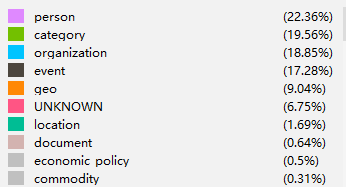
\includegraphics[width=0.75\textwidth]{img/senat_entity_type.png}
\caption{Les types d'entités les plus représentés – Graphe du Sénat}
\end{figure}


\begin{figure}
\centering %
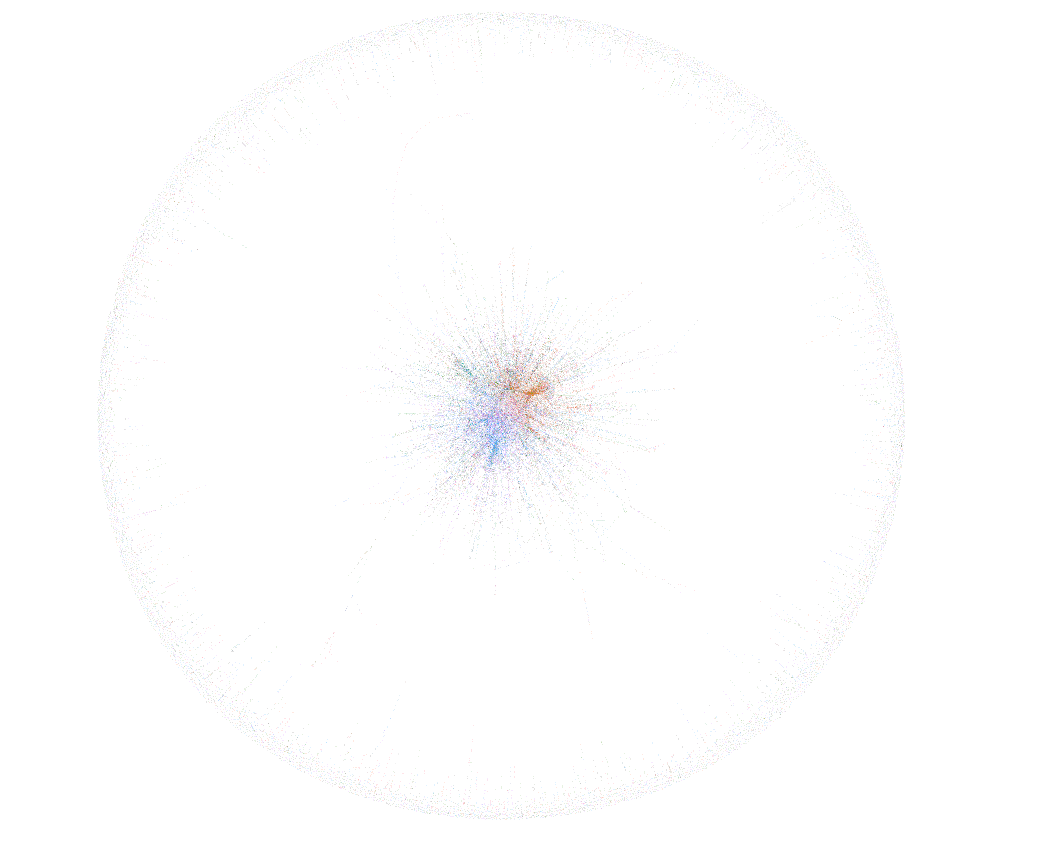
\includegraphics[width=0.75\textwidth]{img/senat_general_view.png}
\caption{Vue générale – Graphe du Sénat}
\end{figure}



\begin{figure}
\centering %
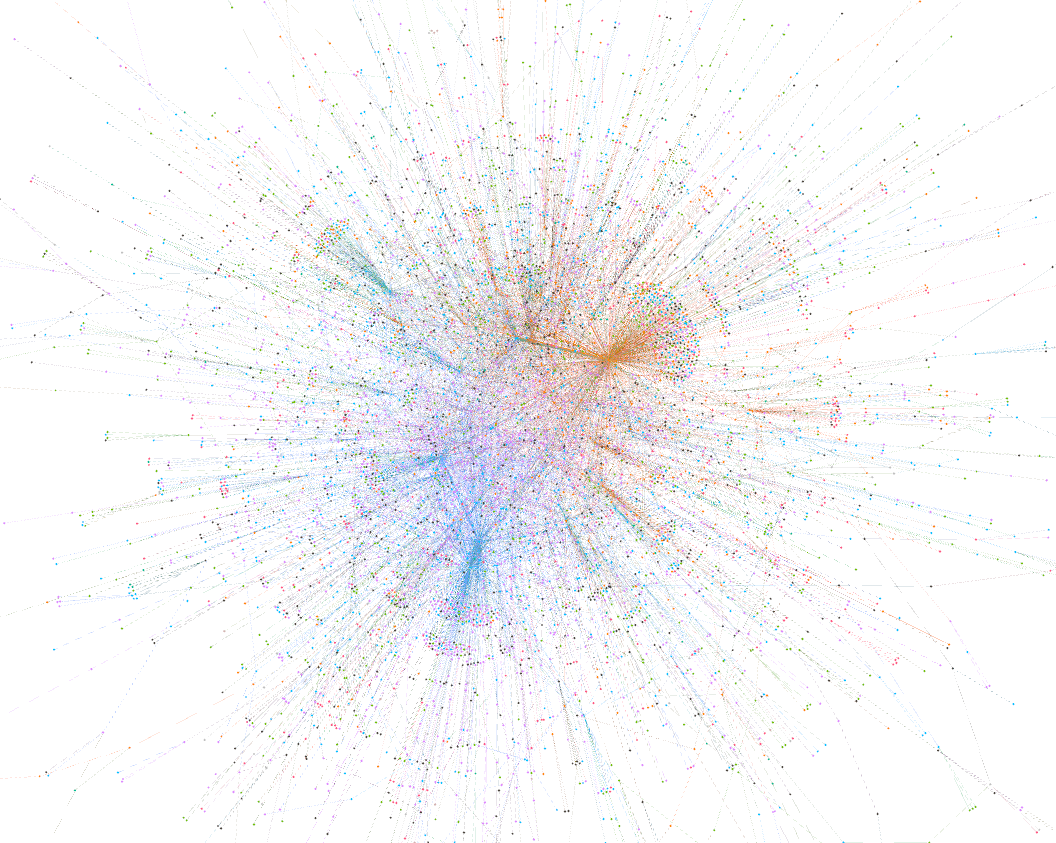
\includegraphics[width=0.75\textwidth]{img/senat_close_view.png}
\caption{Centre du graphe - Graphe du Sénat}
\end{figure}

Ensuite, comme le montre la figure 4.7, dans le graphe du Sénat le nombre d'arêtes est lui aussi inférieur au nombre de nœuds ; même si cet écart est moins marqué, on observe qu'un nombre non négligeable de nœuds non connectés se retrouve écarté vers la périphérie du graphe après réarrangement par l'algorithme de Hu, ce schéma de distribution est similaire à celui de la Chambre. La partie centrale du graphe est représentée à la figure 4.8.



\begin{figure}
\centering %
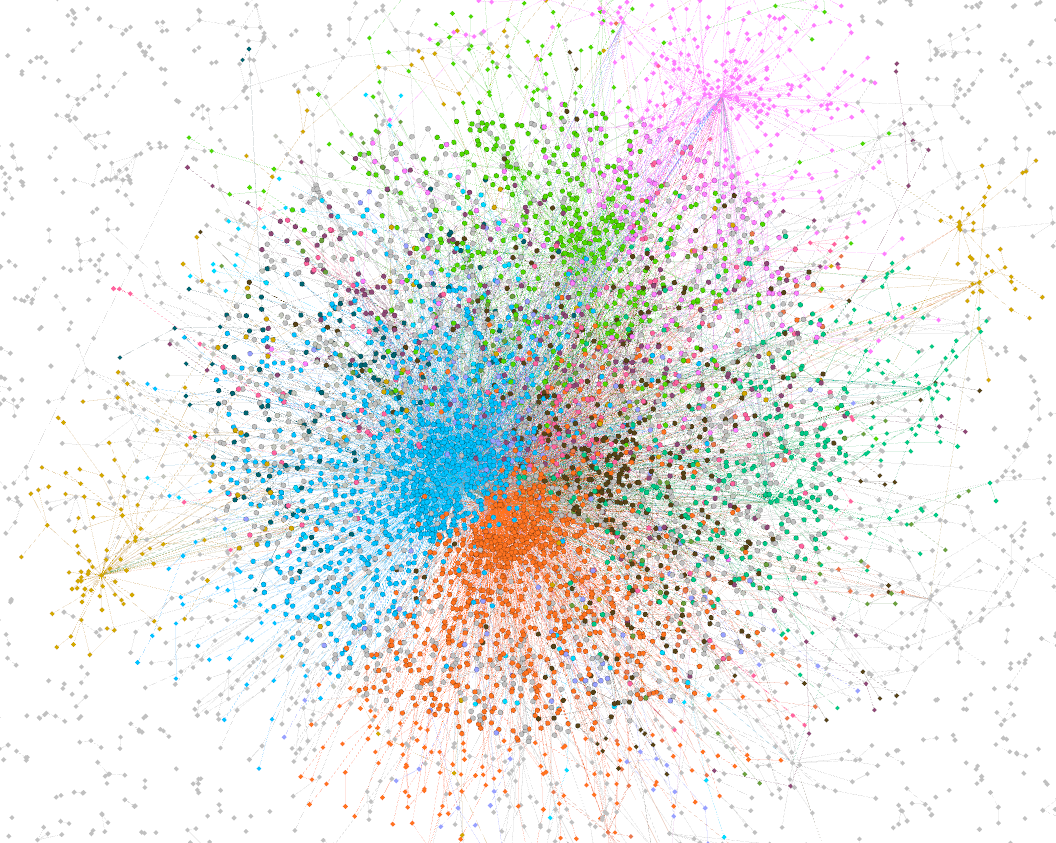
\includegraphics[width=0.75\textwidth]{img/senat_openord.png}
\caption{La distribution des nœuds réorganisée par OpenORD – Graphe du Sénat}
\end{figure}

\begin{figure}
\centering %
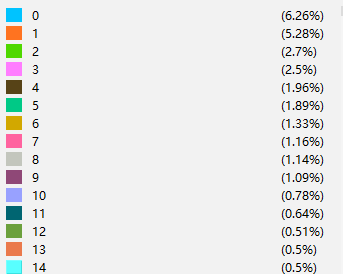
\includegraphics[width=0.75\textwidth]{img/senat_cluster.png}
\caption{Proportion du nombre de nœuds par cluster – Graphe du Sénat}
\end{figure}

Nous avons ensuite appliqué la même méthodologie pour calculer la distribution des communautés dans le graphe. Avec une résolution fixée à 1, le graphe est partitionné en 9,052 communautés et la métrique quality atteint 0.745, ce dernier chiffre est légèrement supérieur à celui de la Chambre et confirme que la partition en communautés est de bonne qualité. Le coloriage des communautés, puis le traitement OpenORD produisent la distribution des nœuds visible à la figure 4.9. Dans la figure 4.10 nous listons les clusters représentant plus de 0.5 \% du total des nœuds : au total 15 clusters, nombre plus élevé que pour la Chambre. On constate que, comparé à la Chambre, les deux plus grands clusters du Sénat ont une part relative plus élevée, tandis que les autres clusters présentent des proportions plus homogènes. Le tableau 4.7 détaille ces éléments.



\begin{table}[htbp]
\centering
\begin{tabular}{|c|p{12cm}|}
\hline
\textbf{Cluster} & \textbf{Nœuds représentatifs (par fréquence décroissante)} \\
\hline
0 & France (910), Allemagne (159), Société des nations (98), Italie (72), Versailles (48) \\
1 & Sénat (328), Chambre des députés (243), Gouvernement (239), M. le président (103), Commission des affaires étrangères (44) \\
2 & La France (116), L'Allemagne (73), Le Gouvernement (52), La Société des nations (39), Le Gouvernement français (25) \\
3 & la France (151), l'Allemagne (41), la Société des nations (30), le traité de Versailles (23), la guerre (22) \\
4 & M. le ministre des affaires étrangères (86), Le Sénat (78), M. Lémery (62), La Chambre des députés (60), Londres (26) \\
5 & le Sénat (61), le Gouvernement (50), M. le ministre des finances (41), M. le ministre du commerce (36), la Chambre des députés (34) \\
6 & France (64), Sénat (26), M. le président (16), Allemagne (14), Paris (12) \\
7 & Gouvernement français (75), Henry Bérenger (35), Français (21), Ministre des affaires étrangères (20), M. Briand (20) \\
8 & Hitler (43), Germany (36), M. Hitler (19), Constitutional Convention (19), Reich (14) \\
9 & M. le Président (33), Washington (19), Charles Dumont (16), M. Poincaré (13), Bérenger (13) \\
10 & Paris (65), Louis Barthou (13), Russie (12), Quai d'Orsay (11), Convention d'établissement entre la France et la Roumanie (8) \\
11 & Société des Nations (34), Traité de Versailles (17), Guerre (15), Banque de France (12), Gouvernement des Etats-Unis (8) \\
12 & Government (16), Commission de l'agriculture (12), M. Desjardins (10), M. le ministre du commerce et de l'industrie (9), M. Marcel Donon (9) \\
13 & Chambre des Députés (18), M. Dominique Delahaye (14), M. le rapporteur (14), Gouvernement de la République (9), Royaume-Uni de Grande-Bretagne et d'Irlande du Nord (9) \\
14 & Rome (21), M. Labrousse (11), Convention (10), Le Parlement (8), Berlin (8) \\
\hline
\end{tabular}

\vspace{0.5em}
\caption{Représentants les plus fréquents par cluster – Graphe du Sénat}
\label{tab:clusters-nœuds}
\end{table}

Nous avons d'abord remarqué que la casse des noms de nœuds diffère de celle fournie pour le graphe de la Chambre, nous pouvons attribuer cela à l'incertitude de sortie du LLM. Par souci d'authenticité des données, nous n'avons pas modifié ces formes. Dans le cluster 0 on trouve comme nœuds les plus saillants France, Allemagne, Société des Nations, Versailles, etc. On peut donc interpréter ce cluster comme lié aux affaires diplomatiques françaises, en particulier la diplomatie bilatérale, la diplomatie dans le cadre de la Société des Nations et les questions d'après-guerre : cela illustre l'importance des relations internationales dans les débats du Sénat. Le cluster 1 contient des nœuds associés à la Chambre des députés, au Gouvernement, à la Commission des affaires étrangères, etc. On peut y voir des discussions centrées sur les relations inter-chambres et les rapports gouvernement-parlement.

Dans les autres clusters, le contenu des nœuds renvoie majoritairement aux relations gouvernement-parlement et à la diplomatie française : les clusters 3, 6 et 8 traitent davantage des relations avec l'Allemagne ; les clusters 4 et 13 concernent le Royaume-Uni ; les clusters 9 et 11 abordent des activités diplomatiques liées aux États-Unis ; le cluster 10 concerne la diplomatie vers l'Europe de l'Est ; le cluster 14 inclut Rome et Berlin, pouvant représenter des relations germano-italiennes ; enfin, les clusters 5, 7 et 12 regroupent des nœuds liés à différents ministères. Ceci illustre clairement la composition thématique du graphe.




\begin{table}[ht]
\centering
\begin{tabular}{ll@{\hskip 1cm}ll}
\hline
\textbf{Étiquette du nœud} & \textbf{Nombre d'arêtes} \\
\hline
France & 910 \\
Sénat & 328 \\
Chambre des députés & 243 \\
Gouvernement & 239 \\
Allemagne & 159 \\
la France & 151 \\
La France & 116 \\
M. le président & 103 \\
Société des nations & 98 \\
M. le ministre des affaires étrangères & 86 \\
Le Sénat & 78 \\
Gouvernement français & 75 \\
L'Allemagne & 73 \\
Italie & 72 \\
Paris & 65 \\
France  & 64 \\
M. Lémery & 62 \\
le Sénat & 61 \\
La Chambre des députés & 60 \\
Le Gouvernement & 52 \\
le Gouvernement & 50 \\
Versailles & 48 \\
Angleterre & 46 \\
Commission des affaires étrangères & 44 \\
M. le président du conseil & 43 \\
Hitler & 43 \\
M. le ministre des finances & 41 \\
l'Allemagne & 41 \\
\hline
\end{tabular}

\vspace{0.5em}
\caption{Nœuds avec le plus grand nombre d'arêtes – Graphe du Sénat}
\label{tab:node-edge-count}
\end{table}

Le tableau 4.8 recense les nœuds ayant plus de 40 arêtes. Les nœuds les mieux connectés sont France, Sénat, Chambre des députés et Gouvernement, ce qui confirme l'importance de ces entités dans le corpus et traduit, en partie, la position et la fonction du Sénat dans l'ensemble du système parlementaire. On retrouve également des entités similaires à celles observées pour la Chambre : Allemagne, Société des Nations, M. le ministre des affaires étrangères, Italie, Versailles, Angleterre. Ces nœuds montrent que les discussions du corpus portent principalement sur les relations entre la France et d'autres pays européens, et que la Société des Nations occupe une place notable dans les débats, en lien étroit avec les accords d'après-guerre.



\begin{table}[ht]
\centering
\begin{tabular}{ll@{\hskip 1cm}ll}
\hline
\textbf{Nœud source} & \textbf{Nœud cible} & \textbf{Poids} \\
\hline
France & Société des nations & 959.0 \\
Société des nations & Allemagne & 856.0 \\
Sénat & Chambre des députés & 647.0 \\
France & Allemagne & 557.0 \\
Sénat & Gouvernement & 424.0 \\
Sénat & M. le président & 422.0 \\
France & Gouvernement & 276.0 \\
France & Italie & 269.0 \\
Sénat & France & 235.0 \\
France & Chambre des députés & 203.0 \\
Tokyo & World Athletics Championship & 193.0 \\
France & Belgique & 170.0 \\
France & Espagne & 157.0 \\
Chambre des députés & Gouvernement & 151.0 \\
France & Angleterre & 149.0 \\
Noah Carter & 100m Sprint Record & 149.0 \\
Global Tech Index & Nexon Technologies & 138.0 \\
Noah Carter & Carbon-Fiber Spikes & 122.0 \\
France & Germany & 101.0 \\
\hline
\end{tabular}
\caption{Relations pondérées entre entités – Graphe du Sénat}
\end{table}

Le tableau 4.9 présente les arêtes du graphe du Sénat dont le poids dépasse 100. Comme évoqué précédemment, l'utilisation de LightRAG a conduit à l'inclusion erronée dans le graphe de certains éléments présents dans les exemples de prompt (e. g. World Athletics Championship, Tokyo, Noah Carter, 100m Sprint Record, Global Tech Index) ; ces occurrences proviennent de ces exemples et, par souci d'intégrité, nous ne les avons pas retirées du tableau. Hormis ces artefacts, les résultats confirment les conclusions dégagées dans le chapitre précédent : sur le plan bilatéral, les relations franco-allemandes, franco-italiennes, franco-belges, franco-espagnoles, etc., sont des sujets récurrents au Sénat ; surtout, la Société des Nations joue un rôle central dans la diplomatie française, et figure fréquemment dans les discussions. La relation triadique France–Société des Nations–Allemagne semble ainsi constituer l'un des noyaux relationnels les plus importants du graphe du Sénat.

En somme, l'analyse des deux graphes construits à partir des textes de la Chambre des députés et du Sénat montre que : d'une part, les graphes restituent fidèlement le contenu textuel et reflètent la structure thématique et sémantique du corpus, ce qui constitue une base solide pour nos analyses ; d'autre part, Chambre et Sénat présentent des sujets très proches, ce qui est attendu. Les relations franco-allemandes y apparaissent de façon particulièrement marquante, tandis que les relations européennes et transatlantiques (y compris avec les États-Unis) sont aussi fréquemment discutées. Fait notable pour notre étude, la Société des Nations fait l'objet d'un nombre important de discussions au sein du parlement, et ces discussions sont profondément intégrées au cadre diplomatique entre la France et les autres États, nous approfondirons ce point dans la sous-section suivante.

\subsection{Analyse microstructurelle}

Comme dans la section précédente, nous avons extrait à l'aide de RAG les nœuds liés à la Société des Nations dans le graphe de connaissances, puis nous avons classé, selon le poids de leurs arêtes, les nœuds adjacents de types organisation, géographique, personne et événement en utilisant la même méthode :

\begin{quote}
\texttt{
"League of Nations",\\
"The League of Nations",\\
"League of Nations",\\
"Société des nations",\\
"Société des Nations",\\
"La Société des nations",\\
"la Société des nations",\\
"Société des nations (League of Nations)",\\
"`Société des Nations (League of Nations)",\\
"La Société des nations (The League of Nations)",\\
"la Société des Nations (League of Nations)",\\
"La Société des Nations (League of Nations)".
}
\end{quote}




\begin{table}[htbp]
\centering
\begin{tabular}{ll@{\hskip 1cm}ll}
\hline
\textbf{Nœud} & \textbf{Type} & \textbf{Poids} \\
\hline
France & geo & 959.0 \\
Allemagne & geo & 856.0 \\
Genève & geo & 77.0 \\
La France & geo & 28.0 \\
Gouvernement français & organization & 26.0 \\
la France & organization & 26.0 \\
Autriche & geo & 26.0 \\
France & geo & 25.0 \\
les Etats-Unis & organization & 18.0 \\
Genève & geo & 18.0 \\
Le Conseil de la Société des nations & organization & 18.0 \\
France, État membre de la Société des Nations & organization & 18.0 \\
France & geo & 16.0 \\
Conseil de la Société des nations & organization & 16.0 \\
Banque de France & organization & 16.0 \\
Le Gouvernement & organization & 16.0 \\
L'Assemblée des nations & organization & 16.0 \\
Genève  & geo & 16.0 \\
Briand-Kellogg & organization & 16.0 \\
l'Italie & geo & 16.0 \\
Allemagne & geo & 15.0 \\
France & geo & 14.0 \\
France  & geo & 14.0 \\
commission des affaires étrangères & organization & 10.0 \\
Ligue des nations & organization & 10.0 \\
Cour Permanente de Justice de la Haye & organization & 10.0 \\
Belgique & geo & 9.0 \\
Gouvernement & organization & 9.0 \\
le conseil de la Société des nations & organization & 9.0 \\
Commission d'études pour l'union européenne & organization & 9.0 \\
Gazette de Voss & organization & 9.0 \\
Rhénanie & geo & 9.0 \\
Pologne & geo & 9.0 \\
Comité des effectifs de Genève & organization & 9.0 \\
République fédérale d'Autriche & organization & 9.0 \\
Commission de gouvernement du territoire & organization & 9.0 \\
Mondiaux & geo & 9.0 \\
Le Gouvernement français & organization & 9.0 \\
United States & geo & 9.0 \\
Government & organization & 9.0 \\
Les pays nordiques & geo & 9.0 \\
Le comité des festivals internationaux de Genève & organization & 9.0 \\
Afrique du Nord & geo & 9.0 \\
The Government & organization & 9.0 \\
Ligue des Nations & organization & 9.0 \\
Conseil de la Société des Nations & organization & 9.0 \\
Europe  & geo & 9.0 \\
Gouvernement (Government) & organization & 9.0 \\
L'Angleterre (England) & geo & 9.0 \\
\hline
\end{tabular}
\caption{Nœuds (geo et organization) liés à la Société des Nations les plus importants – Graphe du Sénat}
\end{table}

Dans le tableau 4.10, nous pouvons observer de nombreux noms de pays déjà présents dans la Chambre, avec l'Allemagne toujours en première position en termes de poids, et dont la valeur est plusieurs fois supérieure à celle des autres pays, excepté la France. Cela souligne très fortement l'importance des relations entre l'Allemagne et la Société des Nations dans les débats du Sénat. En outre, contrairement à la liste de la Chambre où apparaissaient le Japon et la Turquie, la liste du Sénat se compose presque exclusivement de pays européens ainsi que des États-Unis, ce qui reflète en partie l'orientation des débats au Sénat. 

Ensuite, en analysant les descriptions des arêtes entre ces nœuds de la même manière, nous constatons que leur contenu est quasi identique à celui observé dans la Chambre. Par conséquent, nous pouvons considérer que les textes du Sénat sur les relations entre la Société des Nations et les autres pays sont globalement cohérents avec ceux de la Chambre, indiquant un consensus entre les deux assemblées sur le rôle de la Société des Nations en diplomatie.




\begin{table}[htbp]
\centering
\begin{tabular}{ll@{\hskip 1cm}ll}
\hline
\textbf{Nœud} & \textbf{Poids} \\
\hline
Léon Bourgeois & 28.0 \\
Pierre Laval & 23.0 \\
M. Lémery & 20.0 \\
le président Wilson & 20.0 \\
Le secrétaire général do la Société des nations & 20.0 \\
L'orateur & 18.0 \\
M. le ministre des affaires étrangères & 16.0 \\
M. Dominique Delahaye & 16.0 \\
Paul-Boncour & 16.0 \\
M. le président de la commission des affaires étrangères & 15.0 \\
Marcel Cachin & 14.0 \\
M. Armbruster & 12.0 \\
Henry Bérenger & 10.0 \\
Roosevelt & 10.0 \\
M. Herriot & 9.0 \\
M. le chancelier Hitler & 9.0 \\
M. Bénès & 9.0 \\
Aristide Briand & 9.0 \\
Maréchal Foch & 9.0 \\
Le Président Laval & 9.0 \\
M. le président du conseil & 8.0 \\
M. le ministre des finances & 8.0 \\
M. François-Saint-Maur & 8.0 \\
M. Paul-Boncour & 8.0 \\
Paul Laffont & 8.0 \\
Chancelier d'Autriche & 8.0 \\
Victor Bérard & 8.0 \\
M. Lesaché & 8.0 \\
Curtius & 8.0 \\
M. Labrousse & 8.0 \\
Clemenceau & 8.0 \\
M. le comte Louis de Blois & 8.0 \\
le président de la plus Igrandie République du monde & 8.0 \\
M. Lémery & 8.0 \\
Léon Bérard & 7.0 \\
M. Camille Chautemps & 7.0 \\
Gautherot & 7.0 \\
Dominique Delahaye & 7.0 \\
partisans d'une Société des nations & 7.0 \\
Kellogg & 7.0 \\
M. Benès & 7.0 \\
M.François-Saïnt-Maur & 6.0 \\
M.HenrydeJtmvene & 6.0 \\
M. Litvinoff & 6.0 \\
\hline
\end{tabular}
\caption{Nœuds (person) liés à la Société des Nations les plus importants – Graphe du Sénat}
\end{table}


\begin{table}[htbp]
\centering
\begin{tabular}{p{8cm}r}
\hline
\textbf{Nœud} &  \textbf{Poids} \\
\hline
Versailles & 46.0 \\
Pacte de la Société des nations & 28.0 \\
Désarmement & 22.0 \\
Arbitrage sino-japonais & 20.0 \\
Paix & 18.0 \\
Pacte Kellogg & 18.0 \\
Le conseil de la Société des nations & 14.0 \\
World War I & 12.0 \\
plébiscite & 10.0 \\
Le pacte rhénan de Locarno (...) & 10.0 \\
Loi du 31 mars 1928 & 10.0 \\
confernce internationale du travail & 10.0 \\
Les conférences de la Société des nations & 10.0 \\
Le pacte de Paris & 10.0 \\
Accord de Londres & 9.0 \\
Accords de la Haye & 9.0 \\
Pacte de Genève & 9.0 \\
Conférence de Londres & 9.0 \\
Le traité de Locarno & 9.0 \\
Paris Pact & 9.0 \\
Première Guerre mondiale & 9.0 \\
L'agression non provoquée & 9.0 \\
Le Pacte de Paris & 9.0 \\
Treaty of Geneva & 9.0 \\
Pact of Paris & 9.0 \\
le pacte de Paris & 9.0 \\
le traité de Versailles & 8.0 \\
Treaty of Versailles & 8.0 \\
le traité de Paris & 8.0 \\
Washington Treaty & 8.0 \\
Confernce du désarmement & 8.0 \\
la conférence du désarmement & 8.0 \\
Treaty of Versailles  & 8.0 \\
Paris Peace Conference & 7.0 \\
Trianon & 7.0 \\
les négociations avec l'Allemagne & 7.0 \\
\hline
\end{tabular}
\caption{Nœuds (event) liés à la Société des Nations les plus importants – Graphe du Sénat}
\end{table}

Dans le tableau 4.11, nous voyons les nœuds de type personne adjacents à la Société des Nations dans le corpus du Sénat. Nous remarquons, outre certaines personnes déjà mentionnées dans la Chambre, des figures propres au Sénat telles que M. Dominique Delahaye et M. Lémery. D'après les descriptions des arêtes, ces derniers ont occupé des fonctions liées à la Société des Nations et expriment une opinion globalement positive à son égard. En revanche, pour d'autres personnes comme M. le chancelier Hitler, le contenu des arêtes les décrit comme un défi à la Société des Nations. Ainsi, nous pouvons tirer une conclusion similaire à celle du tableau 4.5.

Dans le tableau 4.12, nous pouvons voir les nœuds de type événement du texte Senat qui sont proches des nœuds de la Société des Nations. Nous constatons que les nœuds de type événement dans Sénat, par rapport à ceux de la Chambre, semblent moins souvent liés à des pactes et des conférences concrètes. En revanche, certains nœuds non liés aux pactes et aux conférences possèdent un poids plus élevé, tels que Désarmement, Arbitrage sino-japonais, Paix, etc. Ce résultat peut en partie être attribué à l'instabilité de sortie du LLM, mais nous pouvons également l'interpréter comme le rôle joué par la Société des Nations sur des sujets plus larges. D'autre part, comme dans les conclusions tirées depuis les textes de la Chambre, nous remarquons que la Société des Nations est également liée à certains consensus et accords conclus en dehors du cadre de la Société des Nations, tels que le Pacte Kellogg-Briand, le Traité de Locarno, etc. On peut considérer que cela représente en réalité le rôle important de la Société des Nations dans les actions diplomatiques à plus grande échelle, et que l'esprit multilatéral qu'elle incarne se manifeste déjà dans de nombreuses pratiques diplomatiques de cette période.

Globalement, les conclusions tirées du Sénat rejoignent celles de la Chambre. Les discussions internes au Sénat sur la politique internationale accordent une place importante à la Société des Nations, et le cadre politique international repose essentiellement sur elle. Ceci peut être vu comme une tentative majeure de mise en œuvre du multilatéralisme, qui s'exprime à travers le cadre de la Société des Nations. Toutefois, le rôle du multilatéralisme et de la Société des Nations semble limité à l'Europe, car les nœuds les plus pondérés montrent peu de pays hors d'Europe, contrairement à la Chambre. De plus, en réalisant le même test que dans la section précédente, nous constatons l'absence de lien entre l'Indochine et la Société des Nations, ce qui semble confirmer notre analyse.
\section{Discussion générale des résultats}

En comparant nos résultats de calcul avec les conclusions déjà présentes dans la littérature, nous pouvons constater que, bien que durant la période 1929-1939 les tensions entre le gouvernement et le parlement, ainsi qu'au sein même du parlement, aient globalement suivi une tendance à la hausse, lorsque nous prenons nos résultats et que nous utilisons l'existence de la Société des Nations comme prisme pour observer l'attitude du parlement face au multilatéralisme, nous constatons que cette attitude est restée positive. Autrement dit, d'après nos résultats, la montée en puissance du gouvernement et la polarisation idéologique n'ont pas entraîné de changement radical dans l'évaluation du multilatéralisme au sein du parlement ; au contraire, lorsque la Société des Nations n'a pas su remplir correctement ses fonctions, des critiques ont bel et bien émergé en son sein.

D'autre part, bien que nous ayons auparavant distingué les événements diplomatiques menés dans le cadre de la Société des Nations de ceux qui se sont déroulés en dehors de ce cadre, nos résultats montrent une présence plus large de la Société des Nations. Comme nous l'avons vu dans la littérature, la Société des Nations n'est pas intervenue formellement dans certains événements diplomatiques, mais les principes et l'esprit qui s'y manifestaient étaient bel et bien liés à elle. Nous pouvons le comprendre à partir des nœuds connectés à celui de la Société des Nations dans le graphe de connaissances. Ainsi, nous pouvons considérer que l'esprit multilatéraliste incarné par la Société des Nations a, dans une certaine mesure, constitué un élément déterminant de l'évaluation positive des pratiques diplomatiques de l'époque, bien que cet esprit ait ensuite été fragilisé et violé.



\chapter{Conclusion}
Dans cette recherche, nous avons tenté de répondre à deux questions : d'une part, savoir si, et comment, le multilatéralisme est apparu dans les débats parlementaires français entre 1929 et 1939, et d'autre part, comment le RAG pourrait être appliqué à la recherche historique.

Tout d'abord, concernant la première question, nos résultats montrent que la Société des Nations, en tant que cadre de résolution des affaires diplomatiques, a occupé une place assez importante dans les débats parlementaires de cette période. En termes quantitatifs, elle a été très fréquemment mentionnée et largement associée à différents pays, personnalités et événements. Du point de vue de l'évaluation, grâce aux résumés générés par les LLMs, nous avons constaté qu'au sein du Parlement, l'idée de traiter et de résoudre les affaires diplomatiques dans le cadre de la Société des Nations était majoritairement présentée de manière positive. Bien que l'efficacité de la Société des Nations ait été mise en doute et critiquée à propos de certains conflits internationaux, tels que la guerre italo-éthiopienne ou l'invasion de la Mandchourie par le Japon, le recours ou non au cadre de la Société des Nations constituait néanmoins un critère essentiel d'évaluation des décisions diplomatiques au Parlement. Étant donné que la Société des Nations incarnait l'esprit de coopération internationale et de diplomatie multilatérale, et qu'elle avait prouvé son utilité après la Première Guerre mondiale, nous avons des raisons de penser qu'elle représentait bel et bien une forme d'esprit multilatéral. Certes, cet esprit restait limité dans son champ d'application, mais il a bel et bien été confirmé dans le Parlement français de cette période par le biais de ce cadre institutionnel.

En ce qui concerne la deuxième question, nous considérons que le RAG présente un potentiel considérable pour de nombreux aspects de la recherche historique, qu'il s'agisse de la recherche documentaire ou de la synthèse d'informations. Un usage approprié peut grandement améliorer l'efficacité du travail de recherche. Plus encore, le RAG est particulièrement bien adapté aux défis posés par les ensembles de données historiques de grande voire très grande échelle. Une structuration judicieuse des documents, combinée à une stratégie de recherche cohérente, permet de réduire considérablement le temps nécessaire à des tâches qui auraient autrefois exigé un travail humain intensif, comme le classement, l'archivage ou l'extraction d'informations. Par ailleurs, les capacités de compréhension sémantique des grands modèles de langage offrent une solution plus abordable à des tâches complexes, par exemple l'analyse de corpus multilingues.

Bien que nous soyons parvenus à une conclusion préliminaire, notre étude présente encore un certain nombre de limites et de faiblesses. Comme nous l'avons indiqué dans la section 3.3.2, la présence massive d'erreurs OCR dans le corpus de base implique que nos données ne sont pas totalement complètes. Ensuite, même si les textes retenus à l'issue de notre sélection finale ont une certaine représentativité, ils ne couvrent pas l'ensemble des documents liés à la politique internationale. En effet, les affaires internationales pouvaient parfois être abordées sous d'autres formes discursives. Une approche plus idéale aurait consisté à lire manuellement un grand nombre de textes afin d'identifier leurs caractéristiques, puis à optimiser la phase d'extraction pour capturer les types de discours encore non inclus. Mais, faute de ressources humaines suffisantes, cela n'a pas été possible, ce qui constitue une limite regrettable. Par ailleurs, l'une des limites méthodologiques les plus importantes de cet article réside dans le fait que, faute de temps et de ressources, nous n'avons pas pris en compte les timestamps lors de la conversion des données textuelles en graphe de connaissances. Cela signifie que le graphe que nous présentons correspond à une forme d'"agrégation moyenne de textes sur plusieurs années", ce qui a conduit à la perte d'une partie précieuse des variations diachroniques. Ainsi, lorsque nous affirmons, sur la base des résultats actuels, que la montée en puissance du gouvernement et la polarisation idéologique n'ont pas modifié l'évaluation du multilatéralisme au sein du parlement, cette conclusion mérite d'être réexaminée dans un cadre analytique plus fin. Dans l'idéal, il s'agirait d'extraire séparément les textes par année, voire par mois, puis de relier entre eux les mêmes nœuds dans les graphes représentant différentes périodes, afin de mettre en évidence les évolutions diachroniques. C'est une approche que nous prévoyons de mettre en œuvre dans nos recherches futures. Enfin, notre recherche ne couvre que la période 1929-1939, et nos conclusions ne valent donc que pour ce laps de temps. Pour parvenir à une vision plus complète, il faudrait élargir l'enquête à une période plus vaste, comme l'ensemble de l'entre-deux-guerres.

Sur le plan technique, nous avons également constaté que le RAG et son application dans un domaine spécifique restent confrontés à de nombreux défis. Tout d'abord, la question des performances : les évaluations montrent que les principales solutions de RAG basées sur des graphes atteignent en moyenne environ 70\% de précision sur des benchmarks tels que GraphRAGBench (pour des questions ouvertes, des QCM, etc.), et que la densité des graphes générés varie fortement\footcite{xiao2025}. Dans notre cas, comment déterminer si un taux de 70\% de précision est acceptable ? Comment traiter les textes négligés par le RAG ? Il s'agit là d'une question méthodologique cruciale. Ensuite, le problème des hallucinations liées aux LLM : bien que le réglage du paramètre température puisse améliorer la standardisation des sorties, une incertitude subsiste. De plus, comme nous l'avons observé dans nos graphiques de résultats, le modèle a inséré dans le graphe final des extraits de texte qui n'étaient utilisés qu'à titre d'exemple dans le prompt, ce qui constitue une erreur sérieuse. Nous espérons trouver une solution à ce problème dans l'avenir. Un autre point important relevé lors de la construction de notre pipeline est la différence de précision selon les cadres utilisés. Par exemple, selon que nous importions un modèle depuis HuggingFace\footcite{2025d}, vLLM\footcite{zotero-794} ou Ollama\footcite{zotero-795}, les graphes générés différaient notablement en nombre de nœuds et d'arêtes. Si l'on ajoute à cela le changement de LLM, la qualité finale du graphe s'en trouve encore plus affectée. La question de savoir comment identifier la meilleure solution nécessite donc de nombreux tests expérimentaux. Enfin, cette question se relie à celle du coût : déployer le RAG dans un contexte de recherche concret exige beaucoup de temps et de ressources financières. Il ne suffit pas d'avoir une infrastructure matérielle puissante : selon la taille du corpus, le temps d'indexation peut varier énormément. Par exemple, indexer l'ensemble des débats parlementaires de 1929 à 1939 pourrait prendre plus d'un mois, sans compter le temps nécessaire aux tests pour identifier la meilleure configuration. Dans un contexte de ressources limitées, le RAG peut donc devenir un choix assez contraignant. En somme, pour une recherche concrète, il est indispensable de trouver un équilibre entre temps de calcul, qualité et coûts, et de proposer un cadre standardisé permettant d'évaluer l'application du RAG et, plus largement, des technologies d'intelligence artificielle, dans le domaine historique et des sciences humaines.

Nous pensons également que notre étude a permis de répondre et de soulever plusieurs questions théoriques importantes. Selon nous, les résultats prometteurs obtenus démontrent l'avantage du RAG par rapport aux LLM à contexte très long pour le traitement de corpus de très grande taille, surtout si l'on considère la dégradation observée de la qualité de génération à mesure que la longueur du contexte augmente\footcite{liu2023}\footcite{hsieh2024}. De plus, l'introduction de la lecture machinique, représentée par le RAG, soulève une question herméneutique : comment positionner cette lecture par rapport à la lecture humaine dans la recherche historique ? Comment évaluer et pondérer leur importance respective ? Il s'agit d'une problématique qui devra être approfondie par des pratiques de recherche diversifiées.

En conclusion, notre étude, bien que limitée et imparfaite, ouvre des pistes importantes. Nous espérons que les recherches futures pourront corriger nos lacunes actuelles et produire des résultats plus fiables.


\printbibliography

\appendix


\backmatter

\listoffigures
\listoftables
\tableofcontents

\end{document}
